%Update 11/03/2023
% Changelog
% v. 1.0 limiti
% v. 2.0 nuovo stile
% v. 3.0 derivate fino a punti di non derivabilità
% v. 4.0 concluse derivate
% v. 5.0 studio di funzione completo con esempi e esercizi svolti
% v. 5.1 minor patch (typo)
% v. 5.2 minor parch (error in definition 1.7.2)
%%%%%%%%%%%%%%%%%%%%%%%%%%%%%%%%%%%%%%%%%%%%%%%%%%%%%%%%%%%%%%%%%%%%%%%%%%%%%%%%%%%%%%%%
\documentclass{book}     %type of document
\usepackage[utf8]{inputenc} %for text encoding
\usepackage{lambdatex} 

\usepackage{tasks}
\usepackage{exsheets}

\makeatletter
\renewcommand*\env@cases[1][1.2]{%
  \let\@ifnextchar\new@ifnextchar
  \left\lbrace
  \def\arraystretch{#1}%
  \array{@{}l@{\quad}l@{}}%
}
\makeatother

\title{Analisi 1}
\author{Davide Borra}
\date{}
\makeatletter
\let\runauthor\@author
\let\runtitle\@title
\renewcommand{\chaptermark}[1]{\markboth{#1}{}}
\renewcommand{\sectionmark}[1]{\markright{#1}}
\renewcommand{\footrulewidth}{0.4pt}

\everymath{\displaystyle}

\begin{document}

\lhead{}
\chead{}
\rhead{Indice}
\rfoot{\runauthor}

\begin{titlepage}
    \newgeometry{left=3cm, right=3cm, bottom=2cm, top =3cm} 
    \pagestyle{empty}
    \begin{center}
        \vspace*{\fill}
        \vspace{0.5cm}
        \textbf{\Huge \runtitle}\\\vspace{5mm}
        \textsc{\Large \runauthor}
        \vspace{5cm}
    \end{center}
    \vspace*{\fill}
    v. 5.2\\
    \rule{0.8\linewidth}{0.5mm}\\
    {\footnotesize\href{mailto:davide.borra@studenti.unitn.it}{davide.borra@studenti.unitn.it} - \href{http://davideborra.github.io}{davideborra.github.io}}
    \restoregeometry
\end{titlepage}
\thispagestyle{empty}
\frontmatter
    \tableofcontents
    \creativecommons
\mainmatter
\lhead{\runtitle}
\chead{}
\rhead{\leftmark\ - \rightmark}
\rfoot{\runauthor}

\chapter{Limiti}
\section{Intervalli in $\mathbb{R}$}
\begin{boxdef}
    Un insieme $A \subset \R$ si dice \textbf{intervallo} se corrisponde ad una semiretta (\textbf{illimitato}) o ad un segmento (\textbf{limitato}) della retta reale
\end{boxdef}
Inoltre:
\begin{itemize}
    \item si dice \textbf{chiuso} se gli estremi sono inclusi nell'intervallo;
    \item si dice \textbf{aperto} se gli estremi sono esclusi nell'intervallo.
\end{itemize}
Gli intervallo limitati corrispondono a segmenti di retta reale di estremi $a$ e $b$ ($b>a$), lunghezza $b-a$ (detta \textbf{ampiezza} dell'intervallo), \textbf{centro} $\frac{b+a}{2}$ e \textbf{raggio} $\frac{b-a}{2}$.
\subsection{Intorni}
\begin{boxdef}
    Dato numero reale $x_0$, un intorno completo di $x_0$ è un qualunque intervallo aperto contenente $x_0$ \[I(x_0)=]x_0-\delta_1;x_0+\delta_2[ ~~~~~~ (\text{con }\delta_1, \delta_2 \in \R_0^+ )\]
\end{boxdef}
\begin{itemize}
    \item \textbf{Intorno destro}: $I^+(x_0)=]x_0;x_0+\delta[$
    \item \textbf{Intorno sinistro}: $I^-(x_0)=]x_0-\delta;x_0[$
\end{itemize}
\subsubsection{Intorni circolari}
    \begin{boxdef}
        Dati un numero reale $x_0$ e un numero reale positivo $\delta$, un intorno circolare di $x_0$ di raggio $\delta$ è l'intervallo aperto $I_\delta (x_0)$ di centro $x_0$ e raggio $\delta$ \[I_\delta(x_0)=]x_0-\delta;x_0+\delta[\]
    \end{boxdef}
\subsubsection{Intorni di $\infty$}
\begin{boxdef}
    Dati due numeri reali $a$ e $b$ con $a<b$ si definisce 
    \begin{itemize}
        \item \textbf{intorno di $-\infty$} un qualsiasi intervallo illimitato inferiormente $]-\infty;a[$
        \item \textbf{intorno di $+\infty$} un qualsiasi intervallo illimitato superiormente $]b;+\infty[$
        \item \textbf{intorno di $\infty$} l'unione di un intorno di $-\infty$ e di un intorno di $+\infty$: $]-\infty;a[\  \cup\  ]b;+\infty[$
    \end{itemize}
\end{boxdef}
\subsection{Insiemi limitati e illimitati, maggiorante, minorante, estremi, massimo, minimo.}
È possibile definire come limitati/illimitati anche insiemi che non sono intervalli. 
\begin{boxdef}
    [Insiemi limitati]
    Un insieme $X\subseteq R$ non vuotoè detto
    \begin{itemize}
        \item \textbf{superiormente limitato} se è possibile determinare un qualsiasi numero reale $\alpha$ tale che $\forall x \in X, x\leq \alpha$. $\alpha$ è detto \textbf{maggiorante} di $X$.
        \item \textbf{inferiormente limitato} se è possibile determinare un qualsiasi numero reale $\beta$ tale che $\forall x \in X, x\geq \beta$. $\beta$ è detto \textbf{minorante} di $X$.
        \item \textbf{limitato} se è limitato sia superiormente che inferiormente.
    \end{itemize}
\end{boxdef}
\begin{boxdef}
    [Insiemi illimitati]
    Un insieme $X\subseteq R$ non vuoto è detto 
    \begin{itemize}
        \item \textbf{superiormente illimitato} se $\forall \alpha \in \R, \exists x \in X : x>\alpha$
        \item \textbf{inferiormente illimitato} se $\forall \beta \in \R, \exists x \in X : x<\beta$
        \item \textbf{illimitato} si è illimitato sia inferiormente che superiormente.
    \end{itemize}
\end{boxdef}

Se un insieme è limitato superiormente/inferiormente è possibile definire minimo e massimo è possibile quindi definire massimo e minimo di un insieme (attenzione, non è detto che tutti gli insiemi limitati ammettano massimo/minimo.)
\begin{boxdef}[Massimo]
    Dati un insieme $X\subseteq R$ e un numero reale $M$, esso si dice \textbf{massimo} di $X$ se 
    \begin{tasks}[label={\roman*)}](2)
        \task $\forall x\in X, M\geq x $ (è maggiorante)
        \task $M\in X$ (appartiene all'insieme).
    \end{tasks}
    Si indica $M=\max X$.
\end{boxdef}
\begin{boxdef}[Minimo]
    Dati un insieme $X\subseteq R$ e un numero reale $m$, esso si dice \textbf{minimo} di $X$ se 
    \begin{tasks}[label={\roman*)}](2)
        \task $\forall x\in X, m\leq x $ (è minorante)
        \task $m\in X$ (appartiene all'insieme)
    \end{tasks}
    Si indica $M=\min X$.
\end{boxdef}
Tuttavia non è possibile determinare massimo e minimo per, ad esempio, intervalli aperti. Abbiamo quindi bisogno di qualcos'altro che funzioni sempre, definiamo quindi gli estremi inferiore e superiore di un insieme.

\begin{boxdef}[Estremo superiore]
    Dato un insieme $X$ superiormente limitato, si dice \textbf{estremo superiore} di $X$ il minimo dei suoi maggioranti
    \[\inf X = \min\{M\in \R : M \text{ è maggiorante di }X\}\]
    Se $X$ è superiormente illimitato, si definisce $\sup X = +\infty$.
\end{boxdef}
\paragraph{Caratterizzazione di $\sup X$}
Si dimostra che la seguente definizione di $\sup$ è equivalente alla precedente: dato un insieme $X$ superiormente limitato, un numero reale $M$ si dice estremo superiore di $X$ se e solo se 
\begin{enumerate}[label={\roman*)}]
    \item $\forall x\in X, M\geq x $ (è maggiorante)
    \item $\forall \varepsilon >0 \exists x\in X: x>M-\varepsilon$ (è il minore dei maggioranti)
\end{enumerate}

\begin{boxdef}[Estremo inferiore]
    Dato un insieme $X$ inferiormente limitato, si dice \textbf{estremo inferiore} di $X$ il massimo dei suoi minoranti
    \[\inf X = \max\{m\in \R : m \text{ è minorante di }X\}\]
    Se $X$ è inferiormente illimitato, si definisce $\inf X = -\infty$.
\end{boxdef}

\paragraph{Caratterizzazione di $\inf X$}
Si dimostra che la seguente definizione di $\inf$ è equivalente alla precedente: dato un insieme $X$ inferiormente limitato, un numero reale $m$ si dice estremo inferiore di $X$ se e solo se 
\begin{enumerate}[label={\roman*)}]
    \item $\forall x\in X, m\leq x $ (è minorante)
    \item $\forall \varepsilon >0 \exists x\in X: x<m+\varepsilon$ (è il maggiore dei minoranti)
\end{enumerate}
\subsection{Punti di accumulazione e punti isolati}
\begin{boxdef}[Punto isolato]
    Sia $x_0\in X\subseteq\R$, allora $x_0$ si definisce punto isolato di $X$ se esiste un intorno $I(x_0)$ che non contiene altri elementi di $X$.
\end{boxdef}
\begin{boxdef}[Punto di accumulazione]
    Sia $ X\subseteq\R$, allora $x_0\in \R$ si definisce punto di accumulazione di $X$ se ogni intorno completo $I(x_0)$ contiene altri infiniti elementi di $X$,\\
    \textbf{equivalentemente} se ogni intorno completo $I(x_0)$ contiene almeno un altro elemento di $X$.
\end{boxdef}
\begin{boxdef}[Insieme derivato]
    Dato un insieme $A\subseteq R$, si definisce \textbf{insieme derivato} di $A$, l'insieme $DA$ contenente tutti e soli i suoi punti di accumulazione.
\end{boxdef}
\begin{ex}[
    Dato l'insieme \[A =\left\{x\in \R\;\bigg|\;x =\frac{n + 1}{n}, n\in \N_{ > 0}\right\}\]
    \begin{tasks}(1)
        \task precisare se è limitato,
        \task rappresentarlo graficamente,
        \task determinare $\sup A$ e $\inf A$, specificando se sono massimo e minimo,
        \task indicare punti di accumulazione e punti isolati.
    \end{tasks}
]
     \begin{enumerate}[label=\textit{\alph*)}]
        \item Cominciamo espandendo alcuni elementi dell'insieme
        \[A =\left\{1, \frac{3}{2}, \frac{4}{3}, \frac{5}{4}, \frac{6}{5}, \dots \right\}\]
        Osserviamo facilmente che è limitato inferiormente superiormente
        \item Anche qui calcoliamo i primi elementi, in modo da poterli rappresentare:
        \begin{center}
            \renewcommand{\arraystretch}{1.5}
            \everymath{\textstyle}
            \begin{tabular}[h]{|c||c|c|c|c|c|}
                \hline
                $n$&$1$&$2$&$3$&$4$&$5$\\\hline
                $x$&$2$&$\frac{3}{2}$& $\frac{4}{3}$& $\frac{5}{4}$& $\frac{6}{5}$\\ \hline
            \end{tabular}\\
            \begin{tikzpicture}[line cap=round,line join=round,>=triangle 45,x=1.0cm,y=1.0cm]
                \begin{axis}[
                x=1.0cm,y=1.0cm,
                axis lines=middle,
                ymajorgrids=true,
                xmajorgrids=true,
                xmin=-0.5,
                xmax=10.5,
                ymin=-0.5,
                ymax=3.5,
                xlabel=$n$,
                ylabel=$x$,
                xtick={-0.0,1.0,...,10.0},
                ytick={-0.0,1.0,...,3.0},]
                \clip(-0.5,-0.5) rectangle (10.5,3.5);
                \draw[line width=1.pt,dashed,color=teal,smooth,samples=100,domain=1.0000000399999984:10.5] plot(\x,{((\x)+1)/(\x)+0*sqrt((\x)-1)});
                \draw [line width=1.pt,dashed,color=teal,domain=0.0:10.5] plot(\x,{(--0.5-0.*\x)/0.5});
                \begin{scriptsize}
                \draw [fill=teal] (1.,2.) circle (2.5pt);
                \draw [fill=teal] (2.,1.5) circle (2.5pt);
                \draw [fill=teal] (3.,1.3333333333333333) circle (2.5pt);
                \draw [fill=teal] (4.,1.25) circle (2.5pt);
                \draw [fill=teal] (5.,1.2) circle (2.5pt);
                \draw [fill=teal] (6.,1.1666666666666667) circle (2.5pt);
                \draw [fill=teal] (7.,1.1428571428571428) circle (2.5pt);
                \draw [fill=teal] (8.,1.125) circle (2.5pt);
                \draw [fill=teal] (9.,1.1111111111111112) circle (2.5pt);
                \draw [fill=teal] (10.,1.1) circle (2.5pt);
                \draw [fill=teal] (11.,1.0909090909090908) circle (2.5pt);
                \draw [fill=teal] (12.,1.0833333333333333) circle (2.5pt);
                \draw [fill=teal] (13.,1.0769230769230769) circle (2.5pt);
                \draw [fill=teal] (14.,1.0714285714285714) circle (2.5pt);
                \draw [fill=teal] (15.,1.0666666666666667) circle (2.5pt);
                \end{scriptsize}
                \end{axis}
                \end{tikzpicture}
        \end{center}
        \item Dal disegno si vede chiaramente che \[\sup A = 2 =\max A,\]
        inoltre osserviamo che \[x =\frac{n + 1}{n} =\frac{n}{n} + \frac{1}{n} = 1 + \frac{1}{n}\underset{n\to +\infty}{\xrightarrow{\hspace{1cm}}}1\]
        quindi 
        \[\inf A = 1\qquad\qquad \nexists \min A\]
        \item Osserviamo che qualsiasi punto dell'insieme consideriamo esiste un suo intorno (ad esempio l'intorno circolare di raggio $\textstyle \frac{1}{2}$), per cui tutti i punti dell'insieme sono punti isolati. Osserviamo inoltre che i punti si \say{addensano} intorno a $1$, per cui ogni intorno di $1$ contiene almeno un punto dell'insieme, per cui $x=1$ è un punto di accumulazione per l'insieme $A$.
     \end{enumerate}
\end{ex}
\section{Definizione di limite}
\begin{boxdef}[Definizione unificata di limite]
    Sia $f:X\subset\R\to \R$, $x_0\in \R^\ast$ punto di accumulazione per $X$, allora $l\in \R^\ast$ si dice \underline{limite per $x$ che tende a $x_0$ di $f(x)$} e si scrive
    \[\lim_{x\to x_0}f(x) = l\qquad\qquad\qquad \left(f(x)\underset{x\to x_0}{\xrightarrow{\hspace{1cm}}}l\right)\]
    se
    \[\forall I(l)\ \exists I(x_0) \ :\ f(x)\in I(l)\ \forall x \in I(x_0)\setminus \{x_0\}\]
\end{boxdef}
Definiamo inoltre i limiti destro e sinistro, che si ottengono sostituendo nella definizione precedente a $I(x_0)$, 
\[\begin{array}{lll}
    \text{Limite sinistro:} & \lim_{x \to x_0^-}f(x) = l \qquad &I^-(x_0)\\
    \text{Limite destro:} & \lim_{x \to x_0^+}f(x) = l & I^ +(x_0)
\end{array}\]
Analogamente definiamo i limiti per eccesso e per difetto, che si ottengono sostituendo nella definizione precedente a $I(l)$, 
\[\begin{array}{lll}
    \text{Limite per eccesso:} & \lim_{x \to x_0}f(x) = l^+\qquad &I^ + (l)\\
    \text{Limite per difetto:} & \lim_{x \to x_0}f(x) = l^-  & I^ - (l)
\end{array}\]

Vediamo ora qualche applicazione delle definizioni di limite a casi particolari:
\begin{itemize}
    \item Limite $+\infty$ per $x\to x_0$: $\lim_{x\to x_0}f(x)=+\infty$
    \[\forall M > 0\ \exists \delta > 0\ :\ f(x) > M\ \forall x \in ] x_0 -\delta, x_0 +\delta[\]
    \item Limite finito per $x\to +\infty$: $\lim_{x\to +\infty}f(x)=l$
    \[\forall \varepsilon > 0\ \exists c > 0\ :\ |f(x) - l |< \varepsilon \ \forall x \in ] c, \infty[\]
    \item Limite $+\infty$ per $x\to +\infty$: $\lim_{x\to +\infty}f(x)=+\infty$
    \[\forall M > 0\ \exists c > 0\ :\ f(x) > M\ \forall x \in ] c,\infty[\]
    \item Limite finito per $x\to x_0$: $\lim_{x\to x_0}f(x)=l$
    \[\forall \varepsilon > 0\ \exists \delta > 0\ :\ |f(x) - l |< \varepsilon \ \forall x \in ] x_0 -\delta, x_0 + \delta[\]
\end{itemize}

\begin{ex}[
    Verificare il seguente limite mediante definizione:
    \[\lim_{x\to -\infty}\frac{2x - 1}{x + 1} = 2\]
]
    Cominciamo determinando il dominio: $\dom f = x+1\neq 0\ \Harr\ x\neq -1$. Ora rappresentiamo il grafico della funzione, osserviamo che si tratta di un'omografica con asintoti $y=2$ e $x=-1$:\\
    \begin{center}
        \begin{tikzpicture}[scale=0.8, line cap=round,line join=round,>=triangle 45,x=1.0cm,y=1.0cm]
            \begin{axis}[
            x=1.0cm,y=1.0cm,
            axis lines=middle,
            ymajorgrids=true,
            xmajorgrids=true,
            xmin=-5.5,
            xmax=5.5,
            ymin=-2.5,
            ymax=6.5,
            xtick={-5.0,-4.0,...,5.0},
            ytick={-2.0,-1.0,...,6.0},]
            \clip(-5.5,-2.5) rectangle (5.5,6.5);
            \draw[line width=1.5pt,color=teal,smooth,samples=100,domain=-5.5:-1.1] plot(\x,{(2*(\x)-1)/((\x)+1)});
            \draw[line width=1.5pt,color=teal,smooth,samples=100,domain=-0.9:5.5] plot(\x,{(2*(\x)-1)/((\x)+1)});
            \draw [line width=1.pt,dash pattern=on 3pt off 3pt,color=red] (-1.,-2.5) -- (-1.,6.5);
            \draw [line width=1.pt,dash pattern=on 3pt off 3pt,color=red,domain=-5.5:5.5] plot(\x,{(--2.-0.*\x)/1.});
            \draw [color=teal](-2.5518824196978303,4.217038073385454) node[anchor=north west] {$y=\frac{2x - 1}{x + 1}$};
            \draw (-0.0894460540647984,1.1015799091315117) node[anchor=north west] {$\left(\frac{1}{2},0\right)$};
            \draw (0.01939091237202069,-0.816671624317422) node[anchor=north west] {$(0,-1)$};
            \draw [color=red](-0.9601417855593511,6.121684986029785) node[anchor=north west] {$x=-1$};
            \draw [color=red](4.100777153752737,2.5436697144193627) node[anchor=north west] {$y=2$};
            \begin{scriptsize}
            \draw [fill=black] (0.,-1.) circle (2.0pt);
            \draw [fill=black] (0.5,0.) circle (2.0pt);
            \end{scriptsize}
            \end{axis}
            \end{tikzpicture}
    \end{center}
    Recuperiamo la definizione di limite
    \[\forall \varepsilon > 0\ \exists I( -\infty)\ :\ \left|\frac{2x - 1}{x + 1} - 2\right|<\varepsilon \ \forall x \in I( -\infty)\]
    e svolgiamo la disequazione.
    \[\begin{cases} \left|\frac{2x - 1}{x + 1} - 2\right|<\varepsilon\\x\neq - 1 \end{cases}\qquad \begin{cases}\left|\frac{\cancel{2x} - 1 - \cancel{2x} - 2}{x + 1}\right|<\varepsilon \\ x\neq - 1\end{cases}\]
    \[\begin{cases}[2] -\frac{3}{x + 1} <\varepsilon \\  -\frac{3}{x + 1} >-\varepsilon\\x\neq 0\end{cases}\qquad \begin{cases}[2] \frac{ -3 -\varepsilon x -\varepsilon}{x + 1} < 0 \\  \frac{ -3 +\varepsilon x +\varepsilon}{x + 1} > 0\\x\neq 0\end{cases} \]
    Separando le due disequazioni
    \begin{enumerate}[label={\Roman*)\ \ }]
        \item $\frac{ -3 -\varepsilon x -\varepsilon}{x + 1} < 0$\\
        \begin{tikzpicture}
            \node at (0,0.4) [anchor=west]{$-3 -\varepsilon x -\varepsilon>0$};
            \node at (0,-0.4)[anchor=west]{$x+1>0$};
            \node at (4,0.4)[anchor=west]{$x<-1-\frac{3}{\varepsilon}$};
            \node at (4,-0.4)[anchor=west]{$x>-1$};
            \draw[->] (7.5,1)--(11.5,1);
            \draw (8.75,1)node [above]{$\textstyle-1-\frac{3}{\varepsilon}$}--(8.75,-1);
            \draw (10.25,1) node [above]{$\textstyle-1$}--(10.25,-1);
            \draw[color=red] (7.5, 0.4)--(8.75,0.4) node {$\circ$};
            \draw[color=red, dashed] (8.75, 0.4)--(11.5,0.4);
            \draw[color=red, dashed] (7.5, -0.4)--(10.25,-0.4) node{$\circ$};
            \draw[color=red] (10.25, -0.4)--(11.5,-0.4);
            \node [color=red]at (8.125,-0.8){$\ominus$};
            \node [color=red]at (9.5,-0.8){$+$};
            \node [color=red]at (11,-0.8){$\ominus$};
            \node at (9.5,-1.6){$x <- 1 -\frac{3}{\varepsilon}\ \ \lor\ \ x > 1$};
        \end{tikzpicture}
        \item $\frac{ -3 +\varepsilon x +\varepsilon}{x + 1} > 0$\\
        \begin{tikzpicture}
            \node at (0,0.4) [anchor=west]{$-3 +\varepsilon x +\varepsilon>0$};
            \node at (0,-0.4)[anchor=west]{$x+1>0$};
            \node at (4,0.4)[anchor=west]{$x>-1+\frac{3}{\varepsilon}$};
            \node at (4,-0.4)[anchor=west]{$x>-1$};
            \draw[->] (7.5,1)--(11.5,1);
            \draw (8.75,1)node [above]{$\textstyle-1$}--(8.75,-1);
            \draw (10.25,1) node [above]{$\textstyle-1+\frac{3}{\varepsilon}$}--(10.25,-1);
            \draw[color=red, dashed] (7.5, 0.4)--(10.25,0.4) node{$\circ$};
            \draw[color=red] (10.25, 0.4)--(11.5,0.4);
            \draw[color=red] (7.5, -0.4)--(8.75,-0.4) node {$\circ$};
            \draw[color=red, dashed] (8.75, -0.4)--(11.5,-0.4);
            \node [color=red]at (8.125,-0.8){$\oplus$};
            \node [color=red]at (9.5,-0.8){$-$};
            \node [color=red]at (11,-0.8){$\oplus$};
            \node at (9.5,-1.6){$x <- 1\ \ \lor\ \ x >- 1 +\frac{3}{\varepsilon}$};
        \end{tikzpicture}
    \end{enumerate}
    In conclusione
    \[\begin{cases} 
        x <- 1 -\frac{3}{\varepsilon} \lor x > 1\\
        x <- 1 \lor x >- 1 +\frac{3}{\varepsilon}\\
        x\neq - 1
    \end{cases}\qquad 
    x <- 1 -\frac{3}{\varepsilon} \lor x >- 1 +\frac{3}{\varepsilon}
    \]
    Che contiene un intorno di $-\infty$, $I(-\infty)=\;\left]-\infty, - 1 -\frac{3}{\varepsilon}\right[$. Il limite è quindi verificato.
\end{ex}
\subsection{Asintoti}
\begin{table}[h]
    \centering
    \begin{tabular}{|m{0.25\textwidth}|m{0.4\textwidth}|m{0.25\textwidth}|}
            \hline
            \textbf{Tipologia} & \textbf{Condizioni} & \textbf{Asintoto}\\
            \hline
            Asintoto verticale&  \[\lim_{x\rightarrow x_0} f(x) = \infty\] & \[x= x_0\]\\\hline
            Asintoto orizzontale & \[\lim_{x\rightarrow \infty} f(x) = l\] & \[y=l\]\\ \hline
            Asintoto obliquo & \[\textnormal{CN: }\lim_{x\rightarrow\infty}f(x) = \infty\]
            \[m=\lim_{x\rightarrow\infty}\frac{f(x)}{x} \qquad ~q=\lim_{x\rightarrow\infty}\left[f(x)-mx\right]\] & \[y=mx+q\] \\ \hline
    \end{tabular}
\end{table}
    \textbf{NB.:} Una funzione può avere anche infiniti asintoti verticali, ma al massimo due tra asintoti orizzontali e asintoti obliqui (uno destro e uno sinistro).
\section{Continuità}
\begin{boxdef}
    Sia $f(x)$ una funzione definita in un intervallo $]a;b[$ e $x_0$ un punto appartenente all'intervallo. $f(x)$ è continua in $x_0$ se e solo se \[\lim_{x\to x_0}f(x)=f(x_0)\]
    La funzione è inoltre continua in $]a;b[$ se è continua in ogni punto $x_0$ dell'intervallo.
\end{boxdef}
Si parla anche di funzioni
\begin{itemize}
    \item \textbf{continue da destra} $x_0$ quando $\lim_{x\to x_0^+}f(x)=f(x_0)$
    \item \textbf{continue da sinistra} $x_0$ quando $\lim_{x\to x_0^-}f(x)=f(x_0)$
\end{itemize}
\section{Primi teoremi sui limiti}
\textbf{N.B.:} I seguenti teoremi valgono per ogni tipologia di limite, sia finito che infinito, e in ogni intorno, sia di un numero reale (anche destro e sinistro) sia di infinito.
    \subsection{Teorema di unicità del limite}
        \begin{shadedTheorem}[Unicità del limite]
            Se una funzione $f(x)$ ha limite finito per $x$ che tende a $x_0$, allora tale limite è unico.
        \end{shadedTheorem}
        \begin{tabular}{m{0.48\textwidth}m{0.48\textwidth}}
            \textit{Ipotesi} & \textit{Tesi}  \\
            $\displaystyle\lim_{x\rightarrow x_0}f(x) = l$ & $l$ è unico
        \end{tabular}
        
        \begin{proof}
        Si procede per assurdo. Si supponga che 
        \[\lim_{x\rightarrow x_0}f(x) = l~~~~\land~~~~ \lim_{x\rightarrow x_0}f(x) = l'\]
        con $l\neq l'$ e $l<l'$.
        Siccome $\varepsilon$ è una quantità arbitraria è possibile porre \[0<\varepsilon<\frac{l-l'}{2}\]
        Si applicano ora le definizioni di limite:
        \[\forall \varepsilon > 0 ~~\exists I(x_0) : |f(x)-l|<\varepsilon~~\forall x \in I(x_0), x\neq x_0\]
        \[\forall \varepsilon > 0 ~~\exists I(x_0) : |f(x)-l'|<\varepsilon~~\forall x \in I(x_0), x\neq x_0\]
        Siccome l'intersezione di due intorni di $x_0$ è ancora un intorno di $x_0$, devono valere entrambe le definizioni:
        \[\left\{\begin{array}{l}
            l-\varepsilon < f(x) < l+\varepsilon\\
            l'-\varepsilon < f(x) < l'+\varepsilon 
        \end{array}\right.\]
        \\Ricordando che $l-\varepsilon<l'-\varepsilon < l+\varepsilon < l'+\varepsilon$ si ottiene:
        \[l'-\varepsilon < f(x) < l+\varepsilon\]
        \[l'-\varepsilon < l+\varepsilon\]
        \[-2\varepsilon<l-l'\]
        \[2\varepsilon > l'-l\]
        \[\varepsilon > \frac{l'-l}{2}\]
        Assurdo: contrasta con quanto posto all'inizio. L'ipotesi per assurdo è falsa, quindi la tesi è dimostrata.\\
        \end{proof}
        
    \subsection{Teorema di permanenza del segno}
        \begin{shadedTheorem}[Permanenza del segno]
            Se il limite di un funzione per $x$ che tende a $x_0$ è un numero $l$ diverso da 0, allora esiste un intorno $I(x_0)$ escluso al più $x_0$ in cui $f(x)$ e $l$ sono entrambi positivi o entrambi negativi.
        \end{shadedTheorem}
        \begin{tabular}{m{0.48\textwidth}m{0.48\textwidth}}
            \textit{Ipotesi} & \textit{Tesi}  \\
            $\displaystyle\lim_{x\rightarrow x_0}f(x) = l ~~ \land ~~ l\neq 0$ & $\exists I(x_0) : f(x) \text{ e } l \text{ sono concordi}~~\forall x \in I(x_0), x\neq x_0$
        \end{tabular}
        
        \begin{proof}
        Espando l'ipotesi:
        \[\forall \varepsilon > 0 ~~\exists I(x_0) : |f(x)-l|<\varepsilon~~\forall x \in I(x_0), x\neq x_0\]
        Siccome $\varepsilon$ è un numero positivo arbitrario pongo 
        \[\varepsilon = |l|\]
        \[|f(x)-l|<\varepsilon\]
        \[-\varepsilon <f(x)-l<\varepsilon\]
        \[l-\varepsilon<f(x)<l+\varepsilon\]
        \begin{itemize}
            \item se $l>0 \rightarrow \varepsilon =l$
            \[l-l<f(x)<l+l\]
            \[0<f(x)<2l\]
            da cui la tesi\[f(x)>0\]
            \item se $l<0 \rightarrow \varepsilon =-l$
            \[l+l<f(x)<l-l\]
            \[2l<f(x)<0\]
            da cui la tesi\[f(x)<0\]
        \end{itemize}
        \end{proof}
        
        \begin{shadedTheorem}[Inverso della permanenza del segno]
            Se una funzione $f(x)$ ammette limite finito $l$ per $x$ che tende a $x_0$ e in un intorno $I(x_0)$ escluso al più $x_0$ è 
            \begin{itemize}
                \item positiva o nulla, allora $l\geq 0$;
                \item negativa o nulla, allora $l\leq 0$.
            \end{itemize}
        \end{shadedTheorem}
        
    \subsection{Teorema del confronto (o dei due carabinieri)}
        \begin{shadedTheorem}[Confronto]
            Siano $g(x)$, $f(x)$ e $h(x)$ tre funzioni definite in uno stesso intorno $I(x_0)$, escluso al più $x_0$. Se per ogni $x\in I(x_0)$ è verificato che \[g(x)\leq f(x) \leq h(x)\]
            e \[\lim_{x\rightarrow x_0} g(x)=l ~~ \land ~~ \lim_{x\rightarrow x_0} h(x)=l\]
            allora è verificato che
            \[\lim_{x\rightarrow x_0} f(x)=l\].
        \end{shadedTheorem}
        \begin{tabular}{m{0.45\textwidth}m{0.45\textwidth}}
            \textit{Ipotesi} & \textit{Tesi}  \\
            \begin{enumerate}
                \item $g(x)$, $f(x)$ e $h(x)$ tre funzioni definite nello stesso intorno $I(x_0)$
                \item $\forall x \in I(x_0) ~~ g(x)\leq f(x) \leq h(x)$
                \item $\displaystyle\lim_{x\rightarrow x_0} g(x)=l ~~ \land ~~ \lim_{x\rightarrow x_0} h(x)=l$
            \end{enumerate} & \[\lim_{x\rightarrow x_0} f(x)=l\]\\
        \end{tabular}
        
        \begin{proof}
            Espando l'ipotesi 3:
            \[\forall \varepsilon > 0 ~~\exists I(x_0) : |g(x)-l|<\varepsilon~~\forall x \in I(x_0), x\neq x_0\]
            \[\forall \varepsilon > 0 ~~\exists I(x_0) : |h(x)-l|<\varepsilon~~\forall x \in I(x_0), x\neq x_0\]
            Di conseguenza 
            \[l-\varepsilon < g(x) <l+\varepsilon\]
            \[l-\varepsilon < h(x) <l+\varepsilon\]
            da cui, per ipotesi 1, 
            \[l-\varepsilon < g(x)\leq h(x) <l+\varepsilon\]
            \[l-\varepsilon < g(x) \leq f(x) \leq h(x) <l+\varepsilon\]
            \[l-\varepsilon < f(x) <l+\varepsilon\]
            La precedente scrittura è equivalente a 
            \[|f(x)-l|<\varepsilon\]
            da cui la tesi.\\
        \end{proof}
\section{Calcolo dei limiti}
\subsection{Funzioni continue e funzioni elementari}
Il limite per $x\to x_0$ di una funzione $f(x)$ continua in $x_0$ è il valore della funzione in $x_0$, 
\[\lim_{x\to x_0}f(x) = f(x_0).\]
Il limite di una funzione elementare può essere ricavato dall'analisi del suo grafico, ad esempio
\[\lim_{x\to -\infty}x^2=+\infty \qquad \qquad \lim_{x\to +\infty}x^2=+\infty\]
\subsection{Algebra dei limiti}
\begin{shadedTheorem}
    Siano $f(x)$, $g(x)$ due funzioni definite in un intorno $I(x_0)\setminus \{x_0\}$ tali che
    \[\lim_{x\to x_0}f(x)=l\qquad \qquad \lim_{x\to x_0}g(x)=m\]
    con $l,m\in \R$, $x_0\in \R^\ast$, allora
    \[\renewcommand{\arraystretch}{2}
        \begin{array}{cr}
        \lim_{x\to x_0}\left[ f(x) + g(x) \right] = l + m\\
        \lim_{x\to x_0}\left[ f(x) - g(x) \right] = l - m\\
        \lim_{x\to x_0}\left[ f(x) \cdot g(x) \right] = l \cdot m\\
        \lim_{x\to x_0}\left[ \frac{f(x)}{g(x)} \right] = \frac{l}{m}\\
        \lim_{x\to x_0}\left[ \frac{1}{g(x)} \right] = \frac{1}{m}\\
        \lim_{x\to x_0}\left[ k\cdot f(x)\right] = k\cdot l & \qquad\text{ con }k\in \R\\
        \lim_{x\to x_0}\left[ f(x) \right]^n = l^n & \text{ con }n\in \R\setminus\{0\}
    \end{array}\]
\end{shadedTheorem}
\begin{shadedTheorem}
    Siano $f(x)$, $g(x)$ due funzioni definite in un intorno $I(x_0)\setminus \{x_0\}$ tali che
        \[\lim_{x\to x_0}f(x)=l\qquad \qquad \lim_{x\to x_0}g(x)=m\]
        con $l,m\in \R^\ast$, $x_0\in \R^\ast$, allora\\
        \begin{itemize}
            \item \textbf{Somma}
            \[\begin{array}{|c|c|c|}
                \hline
                \lim_{x\to x_0}f(x)& \lim_{x\to x_0}g(x)& \lim_{x\to x_0}\left[ f(x)+g(x) \right] \\ \hline\hline
                l & +\infty & +\infty\\
                l & -\infty & -\infty\\
                +\infty & +\infty & +\infty\\
                -\infty & -\infty & -\infty\\
                +\infty & -\infty & F. I. \\\hline
            \end{array}\]
            \item \textbf{Prodotto}
            \[\begin{array}{|c|c|c|}
                \hline
                \lim_{x\to x_0}f(x)& \lim_{x\to x_0}g(x)& \lim_{x\to x_0}\left[ f(x)\cdot g(x) \right] \\ \hline\hline
                l & \infty & \infty\\
                \infty & \infty & \infty\\
                0 & \infty & F. I. \\\hline
            \end{array}\]
            tenendo conto della regola dei segni;
            \item \textbf{Rapporto}
            \[\begin{array}{|c|c|c|}
                \hline
                \lim_{x\to x_0}f(x)& \lim_{x\to x_0}g(x)& \lim_{x\to x_0}\left[ \frac{f(x)}{g(x)} \right] \\ \hline\hline
                l & \infty & 0\\
                l &  0 &\infty \\
                \infty & l & \infty\\
                0 & l & 0\\
                0 & 0 & F. I. \\
                \infty & \infty & F. I. \\\hline
            \end{array}\]
            tenendo conto della regola dei segni;
            \item \textbf{Potenza}
            \[\begin{array}{|c|c|c|}
                \hline
                \lim_{x\to x_0}f(x)& \lim_{x\to x_0}g(x)& \lim_{x\to x_0}\left[ f(x) \right]^{g(x)} \\ \hline\hline
                            & 0         & 1  ~~(0^0~ F.I.)  \\
                0\leq l < 1 &  +\infty  & 0^+    \\
                            & -\infty   & +\infty    \\\hline
                            & 0         & 1 ~~(\infty^0~F.I.) \\
                l\geq 1     & +\infty   & +\infty     \\
                            & -\infty   & 0^+     \\\hline
            \end{array}\]
        \end{itemize}
\end{shadedTheorem}


\subsection{Mediante il teorema del confronto}

\begin{ex}[Si calcoli il valore di $\lim_{x\to +\infty}\frac{\sin x}{x}$]
    Prima di tutto ricordiamo che per definizione di seno $-1\leq \sin x \leq 1$. Siccome stiamo lavorando in un intorno di $+\infty$, possiamo considerare $x>0$, quindi posso dividere tutti i membri per x, ottenendo \[-\frac{1}{x}\leq \frac{\sin x}{x}\leq \frac{1}{x}.\] Siamo quindi riusciti a ricostruire nel membro centrale della disequazione la funzione cercata. Calcoliamo ora i limiti degli estremi:
    \[\lim_{x\to +\infty}\frac{1}{x}=\left[\frac{1}{+\infty}\right]=0^+ ~~~~~~
    \lim_{x\to +\infty}-\frac{1}{x}=\left[-\frac{1}{+\infty}\right]=0^-.\]
    Di conseguenza, per il teorema del confronto \[\lim_{x\to + \infty} \frac{\sin x}{x}=0\]
\end{ex}

\subsection{Forme di indecisione (o forme indeterminate)}
\subsubsection{Forma di indecisione $+\infty-\infty$}
\subsubsection{Se si presenta in una funzione polinomiale}
Per superare queste forme di indecisione, in generale occorre raccogliere il termine di grado massimo. In alternativa esiste una regola pratica ottenuta tramite l'applicazione della gerarchia degli infiniti. In questo caso si considera semplicemente il termine di grado massimo perché il contributo degli altri è trascurabile rispetto ad esso.
\begin{ex}[Calcolare $\lim_{x\to +\infty}(x^2-3x^4+5)$]
\[\begin{aligned}\lim_{x\to +\infty}(x^2-3x^4+5)&=[-\infty+\infty]\overset{\mathrm{FI}}{=}\lim_{x\to +\infty}x^4\left( {\frac{1}{x^2}} -3+\frac{5}{x^5}\right)=\left[ +\infty \left( \cancel{\frac{1}{+\infty}^0}-3+\cancel{\frac{5}{+\infty}^0 }\right) \right]=\\&=[-3(+\infty)]=-\infty\end{aligned}\]
infatti sostituendo dopo aver raccolto ottengo che alcuni termini vanno a 0. Oppure, applicando la regola pratica
\[\lim_{x\to +\infty}(x^2-3x^4+5)=[-\infty+\infty]\overset{\mathrm{FI}}{=}\lim_{x\to +\infty}(-3x^4)=-\infty\]
\end{ex}
\subsubsection{Se si presenta in una funzione irrazionale}
In questo caso si procede raccogliendo il termine doi grado massimo nel radicando, portandolo fuori dal segno di radice e poi raccogliendo nuovamente il termine di grado massimo. Oppure si può procedere applicando la gerarchia al radicando e portando fuori dal segno di radice il termine di grado massimo (si ricorda che $\sqrt{x^{2n}}=|x^n|$). A questo punto dovremmo esserci ricondotti al caso precedente. 
\begin{ex}[Calcolare $\lim_{x\to +\infty}\left(\sqrt{x^2+3}-2x\right)$]
\[\begin{aligned}\lim_{x\to +\infty}\left(\sqrt{x^2+3}-2x\right)=[-\infty+\infty]\overset{\mathrm{FI}}{=}\lim_{x\to +\infty}\left(\sqrt{x^2\left( 1+\frac{3}{x^2} \right)}-2x\right)=\lim_{x\to +\infty}\left(|x|\sqrt{1+\frac{3}{x^2}}-2x\right) =\\= \lim_{x\to +\infty}\left(x\sqrt{1+\frac{3}{x^2}}-2x\right) =\lim_{x\to +\infty}x\left( \sqrt{1+\frac{3}{x^2}-2} \right)=\left[ +\infty\left(\sqrt{1+\cancel{\frac{3}{+\infty}^0}} -2\right)\right]=-\infty\end{aligned}\]
oppure, applicando la regola pratica,
\[\begin{aligned}\lim_{x\to +\infty}\left(\sqrt{x^2+3}-2x\right)&=[-\infty+\infty]\overset{\mathrm{FI}}{=}\lim_{x\to +\infty}\left(\sqrt{x^2}-2x\right)=\lim_{x\to +\infty}(|x|-2x) = \lim_{x\to +\infty}(x-2x) = \\&=\lim_{x\to +\infty}-x=-\infty\end{aligned}\]
\end{ex}
\paragraph{Se il termine sotto radice è il quadrato del termine fuori}
In questo caso, se procedo come nel precedente si origina un'altra forma di indecisione, per cui la soluzione è razionalizzare.
\begin{ex}[Calcolare $\lim_{x\to +\infty}\left(\sqrt{x^2+3}-2x\right)$]
\[\begin{aligned}\lim_{x\to +\infty}\left(\sqrt{4x^2+3}-2x\right)&=[-\infty+\infty]\overset{\mathrm{FI}}{=}\lim_{x\to +\infty}\frac{\left(\sqrt{4x^2+3}-2x\right)\left(\sqrt{4x^2+3}+2x\right)}{\sqrt{4x^2+3}+2x} = \\ &=\lim_{x\to +\infty}\frac{4x^2+3-4x^2}{\sqrt{4x^2+3}+2x}=\lim_{x\to +\infty}\frac{3}{\sqrt{4x^2+3}+2x}=\left[\frac{3}{+\infty+\infty}\right]=0^ +\end{aligned}\]
\end{ex}
\subsubsection{Forma di indecisione $0\cdot \infty$}
Per risolvere questa forma di indecisione è necessario modificare l'espressione analitica della funzione di partenza in modo da rimuovere l'origine della forma di indecisione.
\begin{ex}[Calcolare $\lim_{x\to\frac{3}{2}\pi}\sin^2\left(\frac{3}{2}\pi-x\right)\tg^2x$]
\[\lim_{x\to\frac{3}{2}\pi}\sin^2\left(\frac{3}{2}\pi-x\right)\tg^2x=\left[\sin 0 \cdot \tg \frac{3}{2}\pi\right]=[0\cdot \infty]\overset{\mathrm{FI}}{ = }\]
Ricordando che (per gli angoli associati) $\textstyle\sin^2\left(\frac{3}{2}\pi-x\right)= \left[\sin\left(\frac{3}{2}\pi-x\right)\right]^2=[-\cos x]^2=\cos^2 x$, è possibile riscrivere la funzione come \\ 
\[=\lim_{x\to\frac{3}{2}\pi}\cos^2x~\tg^2x = \lim_{x\to\frac{3}{2}\pi} \cancel{\cos^2x}\cdot\frac{\sin^2x}{\cancel{\cos^2x}}=\left[ \sin^2 \left( \frac{3}{2}\pi \right)=1\right]\]
\end{ex}
\subsubsection{Forma di indecisione $\frac{\infty}{\infty}$}
Si procede raccogliendo il termine di grado massimo (o applicando la gerarchia) sia a numeratore che a denominatore e poi semplificando.
\paragraph{Se si presenta in una funzione razionale fratta}
\begin{ex}[Calcolare $\lim_{x\to +\infty}\frac{3x^4-5x^3+2x-1}{5-2x^4-3x^2}$]
\[\lim_{x\to +\infty}\frac{3x^4-5x^3+2x-1}{5-2x^4-3x^2}=\left[\frac{\infty}{\infty}\right]\overset{\mathrm{FI}}{=}\lim_{x\to +\infty}\frac{\cancel{x^4}\left( 3-\frac{5}{x}+\frac{2}{x^2}-\frac{1}{x^4} \right)}{\cancel{x^4}\left(\frac{5}{x^4} -2 -\frac{3}{x^2}\right)}=\left[ \frac{ 3-\cancel{\frac{5}{+\infty}}+\cancel{\frac{2}{+\infty}}-\cancel{\frac{1}{+\infty}}}{\cancel{\frac{5}{+\infty}} -2 -\cancel{\frac{3}{+\infty}}} \right]=-\frac{3}{2}\]
oppure
\[\lim_{x\to +\infty}\frac{3x^4-5x^3+2x-1}{5-2x^4-3x^2}=\left[\frac{\infty}{\infty}\right]\overset{\mathrm{FI}}{=}\lim_{x\to +\infty}\frac{3x^4}{-2x^4}=-\frac{3}{2}\]
\end{ex}
\textbf{N.B.:} Anche se sia a numeratore che a denominatore si presentano forme di indecisione $-\infty+\infty$ prevale la forma di indecisione $\frac{\infty}{\infty}$
\subsubsection{Se si presenta in una funzione irrazionale fratta}
\begin{ex}[Calcolare $\lim_{x\to +\infty}\frac{1+\sqrt{x^2+1}}{x}$]
\[\begin{aligned}\lim_{x\to +\infty}\frac{1+\sqrt{x^2+1}}{x}&=\left[\frac{\infty}{\infty}\right]\overset{\mathrm{FI}}{=}\lim_{x\to +\infty}\frac{1+\sqrt{x^2\left( 1+\frac{1}{x^2} \right)}}{x}=\lim_{x\to +\infty}\frac{1+|x|\sqrt{1+\frac{1}{x^2}}}{x}=\\&=\lim_{x\to +\infty}\frac{1+x\sqrt{1+\frac{1}{x^2}}}{x}=\lim_{x\to +\infty}\frac{\cancel{x}\left( \frac{1}{x} +\sqrt{1+\frac{1}{x^2}}\right)}{\cancel{x}}=\left[ \cancel{\frac{1}{+\infty}} +\sqrt{1+\cancel{\frac{1}{+\infty}}} \right] =1\end{aligned}\]
oppure
\[\lim_{x\to +\infty}\frac{1+\sqrt{x^2+1}}{x}=\left[\frac{\infty}{\infty}\right]\overset{\mathrm{FI}}{=}\lim_{x\to +\infty}\frac{1+\sqrt{x^2}}{x}=\lim_{x\to +\infty}\frac{1+|x|}{x}=\lim_{x\to +\infty}\frac{1+x}{x}=\lim_{x\to +\infty}\frac{x}{x}= 1\]
\end{ex}
\subsubsection{Forma di indecisione $\frac{0}{0}$}
\subsubsection{Funzioni razionali fratte}
In generale si risolve scomponendo e semplificando
\begin{ex}[Calcolare $\lim_{x\to 2} \frac{3x^2-6x}{x^2-4}$]
\[\lim_{x\to 2} \frac{3x^2-6x}{x^2-4}= \left[\frac{0}{0}\right]\overset{\mathrm{FI}}{=}\lim_{x\to 2}\frac{3x\cancel{(x-2)}}{{\cancel{(x-2)}}(x+2)}=\left[\frac{6}{4}\right]=\frac{3}{2}\]
\end{ex}
\subsubsection{Funzioni irrazionali fratte}
In generale si risolve razionalizzando, scomponendo e semplificando
\begin{ex}[Calcolare $\lim_{x\to 4}\frac{\sqrt{x}-2}{x^2-3x-4}$]
\[\begin{aligned}\lim_{x\to 4}\frac{\sqrt{x}-2}{x^2-3x-4}&= \left[\frac{0}{0}\right]\overset{\mathrm{FI}}{=}\lim_{x\to 4}\frac{(\sqrt{x}-2)(\sqrt{x}+2)}{(x^2-3x-4)(\sqrt{x}+2)}=\lim_{x\to 4}\frac{\cancel{x-4}}{\cancel{(x-4)}(x+1)(\sqrt{x}+2)} =\\&=\lim_{x\to 4}\frac{1}{(x+1)(\sqrt{x}+2)}=\frac{1}{20}\end{aligned}\]
\end{ex}
\begin{ex}[Calcolare $\lim_{x\to27^+}\frac{x-27}{\sqrt[3]{x}-3}$]
\[\lim_{x\to27^+}\frac{x-27}{\sqrt[3]{x}-3}=\left[\frac{0}{0}\right]\overset{\mathrm{FI}}{=}\lim_{t\to3^+}\frac{t^3-27}{t-3}=\lim_{t\to3^+}\frac{\cancel{(t-3)}(t^2+3t+9)}{\cancel{t-3}}=\lim_{t\to3^+}(t^2+3t+9)=27\]
Pongo $\begin{array}{ll}
    t=\sqrt[3]{x}~~~~~ &  x\to27^+\\
    x=t^3 & t\to 3^+
\end{array}$
\end{ex}
\subsubsection{Forme di indecisione $0^0$, $\infty^0$, $1^\infty$}
Generalmente si risolvono applicando l'uguaglianza \[\left[f(x)\right]^{g(x)}=e^{g(x)\ln f(x)}\]
e successivamente applicando all'esponente i metodi risolutivi visti in precedenza.
\begin{ex}[Calcolare $\lim_{x\to0^+}(2x)^{\frac{2}{\ln(2x)}}$]
\[\lim_{x\to0^+}(2x)^{\frac{2}{\ln(2x)}}=\left[0^\frac{2}{-\infty}\right]=\left[0^0\right]\overset{\mathrm{FI}}{=}\lim_{x\to0^+}e^{\frac{2}{\ln(2x)}\ln(2x)}=e^2\]
\end{ex}
\begin{ex}[Calcolare $\lim_{x\to+\infty}x^\frac{1}{\ln x}$]
\[\lim_{x\to+\infty}x^\frac{1}{\ln x}=\left[\infty^0\right]\overset{\mathrm{FI}}{=}\lim_{x\to+\infty}e^{\frac{1}{\ln x}\ln x}=e\]
\end{ex}
\begin{ex}[Calcolare $\lim_{x\to 0^+}\left(\frac{x^2}{4}\right)^\frac{1}{3\ln x}$]
\[\begin{aligned}\lim_{x\to 0^+}\left(\frac{x^2}{4}\right)^\frac{1}{3\ln x}&=\left[0^\frac{1}{-\infty}\right]=\left[0^0\right]\overset{\mathrm{FI}}{=}\lim_{x\to0^+}e^{\ln\left(\frac{x^2}{4}\right)\frac{1}{3\ln x}}=\lim_{x\to0^+}e^{\frac{\ln x^2-\ln4}{3\ln x}} =\\&=\lim_{x\to0^+}e^{\frac{2\ln x}{3\ln x}-\frac{\ln4}{3\ln x}}=\left[e^{\frac{2}{3}+0}\right]=e^\frac{2}{3}\end{aligned}\]
\end{ex}
\subsection{Limiti Notevoli}
\begin{itemize}
\item {$\lim_{x\to 0}\frac{\sin x}{x}=1$}
\begin{proof}
    \[\frac{\sin -x}{-x}=\frac{-\sin x}{-x}=\frac{\sin x}{x}\]
    Siccome la funzione è pari la dimostrazione si svolge solo per $x\to 0^+$. Sulla circonferenza goniometrica considero un angolo $x$. Siccome $x \to 0^+$ posso imporre la condizione $0<x<\frac{pi}{2}$\\
    \begin{figure}[h]
        \centering
            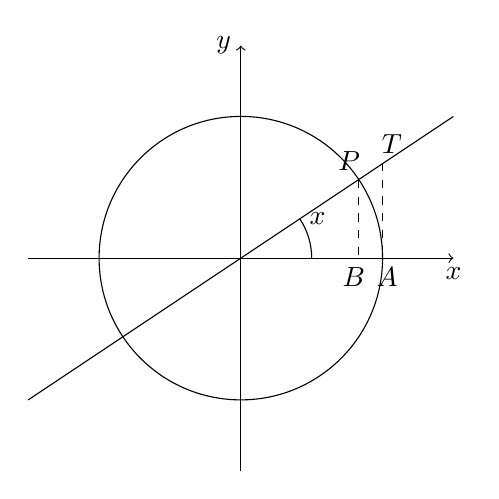
\begin{tikzpicture}[scale=1.8]
                \draw[->] (0,-1.5)--(0,1.5) node[left]{$y$};
                \draw[->] (-1.5,0)--(1.5,0) node[below]{$x$};
                \draw(0,0) circle (1);
                \draw(-1.5,-1)--(1.5,1);
                \draw(0.5,0) arc (0:33.7:0.5) node [right]{$x$};
                \draw[dashed](0.83,0.55) node [above] {$P~~$}to (0.83,0) node [below] {$B~$};
                \draw[dashed](1,0.67) node [above] {$~~T$}to (1,0) node [below] {$~A$};
            \end{tikzpicture}\\
        \caption{La situazione utilizzata per la dimostrazione}
        \label{fig:sinx}
    \end{figure}
    Per definizione si ha che \[\wideparen{PA}=x\]\[\overline{PB}=\sin x\] \[\overline{TA}=\tg x\] 
    Come è chiaramente visibile dalla Figura \ref{fig:sinx} si ha che \[\sin x < x < \tg x\] da cui \[\frac{\sin x}{\sin x}<\frac{ x}{\sin x}<\frac{\tg x}{\sin x}\] \[1<\frac{ x}{\sin x}<\frac{\tg x}{\sin x}\] \[1<\frac{\sin x}{x}<\cos x\]
    Si calcolano ora i limiti delle funzioni che limitano quella studiata
    \[\lim_{x \to 0^+}1=1 ~~~~~ \lim_{x \to 0^+}\cos x=1\]
    da cui per il teorema del confronto \[\lim_{x\to 0^+} \frac{\sin x}{x}=1\] Siccome la funzione è pari vale anche per $x\to0^-$
\end{proof}
\textbf{Osservazioni:}
\begin{itemize}
    \item vale il reciproco: $\lim_{x\to 0}\frac{x}{\sin x}=1$
    \item vale la generalizzazione: $\lim_{f(x)\to 0}\frac{\sin f(x)}{f(x)}=1$
    \item asintotico associato: $\sin x \sim x ~~~~\textnormal{in } I(0)$
\end{itemize}
\item {$\lim_{x\to 0}\frac{\tg x}{x}=1$}~
\\\begin{proof}
    Per definizione $\tg x=\frac{\sin x}{\cos x}$, quindi \[\lim_{x\to 0} \frac{\tg x}{x}=\left[\frac{0}{0}\right]\overset{FI}{=}\lim_{x\to 0} \frac{\sin x}{x \cos x}\underset{LN}{=}\lim_{x\to 0} \frac{1}{\cos x}=1\]
\end{proof}
\textbf{Osservazioni:}
\begin{itemize}
    \item vale il reciproco: $\lim_{x\to 0}\frac{x}{\tg x}=1$
    \item vale la generalizzazione: $\lim_{f(x)\to 0}\frac{\tg f(x)}{f(x)}=1$
    \item asintotico associato: $\tg x \sim x ~~~~\textnormal{in } I(0)$
\end{itemize}

\item {$\lim_{x\to 0}\frac{1-\cos x}{x}=0$}
\begin{proof}
\[\lim_{x\to 0} \frac{1-\cos x}{x}=\left[\frac{0}{0}\right]\overset{FI}{=}\lim_{x\to 0}\frac{(1-\cos x)(1+\cos x)}{x(1+\cos x)}=\lim_{x\to 0}\frac{1-\cos^2 x}{x(1+\cos x)}=\]Per la prima relazione fondamentale della goniometria\[=\lim_{x\to 0}\frac{\sin^2 x}{x(1+\cos x)}\underset{LN}{=}\lim_{x\to 0}\frac{\sin x}{1+\cos x}=\left[\frac{0}{2}\right]=0\]
\end{proof}
\textbf{Osservazioni:}
\begin{itemize}
    \item NON vale il reciproco
    \item vale la generalizzazione: $\lim_{f(x)\to 0}\frac{1-\cos f(x)}{f(x)}=1$
\end{itemize}

\item {$\lim_{x\to 0}\frac{1-\cos x}{x^2}=\frac{1}{2}$}
\begin{proof}
\[\lim_{x\to 0} \frac{1-\cos x}{x^2}=\left[\frac{0}{0}\right]\overset{FI}{=}\lim_{x\to 0}\frac{(1-\cos x)(1+\cos x)}{x^2(1+\cos x)}=\lim_{x\to 0}\frac{1-\cos^2 x}{x^2(1+\cos x)}=\]Per la prima relazione fondamentale della goniometria\[=\lim_{x\to 0}\frac{\sin^2 x}{x^2(1+\cos x)}\underset{LN}{=}\lim_{x\to 0}\frac{1}{1+\cos x}=\frac{1}{2}\]
\end{proof}
\textbf{Osservazioni:}
\begin{itemize}
    \item vale il reciproco: $\lim_{x\to 0}\frac{x^2}{1-\cos x}=1$
    \item vale la generalizzazione: $\lim_{f(x)\to 0}\frac{1- \cos f(x)}{[f(x)]^2}=1$
    \item asintotico associato: $\cos x \sim 1 - x^2 ~~~~\textnormal{in } I(0)$
\end{itemize}

\item {$\lim_{x\to +\infty}\left(1+\frac{1}{x}\right)^{x} = e$}~\vspace{10pt}\\
\textbf{Osservazioni:}
\begin{itemize}
    \item NON vale il reciproco
    \item vale la generalizzazione
\end{itemize}

\paragraph{$\lim_{x\to +\infty}\left(1+\frac{k}{x}\right)^{x} = e^k$}~\vspace{10pt}\\
\textbf{Osservazioni:}
\begin{itemize}
    \item NON vale il reciproco
    \item vale la generalizzazione
\end{itemize}

\paragraph{$\lim_{x\to 0^+}\left(1+kx\right)^{\frac{1}{x}}  e^k$}~\vspace{10pt}\\
\textbf{Osservazioni:}
\begin{itemize}
    \item NON vale il reciproco
    \item vale la generalizzazione
\end{itemize}

\item {$\lim_{x\to 0}\frac{\log_a(1+x)}{x}=\log_ae=\frac{1}{\ln a}~~~~~~~~\textnormal{con }a>0$}
\begin{proof}
\[\lim_{x\to 0}\frac{\log_a(1+x)}{x}=\left[\frac{0}{0}\right]\overset{FI}{=}\lim_{x\to 0}\frac{1}{x}\log_a(1+x)=\lim_{x\to 0}\log_a(1+x)^\frac{1}{x}=\log_ae=\frac{\ln e}{\ln a}=\frac{1}{\ln a}\]
\end{proof}
Particolarizzazione: $\lim_{x\to0}\frac{\ln(1+x)}{x}=1$~\vspace{10pt}\\
\textbf{Osservazioni:}
\begin{itemize}
    \item vale il reciproco
    \item vale la generalizzazione
    \item asintotico associato: $\ln x \sim x - 1 ~~~~\textnormal{in } I(0)$
\end{itemize}

\item {$\lim_{x\to 0}\frac{a^x-1}{x}=\ln a~~~~~~~~\textnormal{con }a>0$}
\begin{proof}
Pongo $t=a^x-1$, quindi $e^x=t+1$ e di conseguenza $x=\log_a (t+1)$. Inoltre, se $x\to 0$, $t\to 0$.
\[\lim_{x\to 0}\frac{a^x-1}{x}=\lim_{t\to 0}\frac{t}{\log_a (t+1)}=\ln a\]
\end{proof}
Particolarizzazione: $\lim_{x\to 0}\frac{e^x-1}{x}=1$~\vspace{10pt}\\
\textbf{Osservazioni:}
\begin{itemize}
    \item vale il reciproco
    \item vale la generalizzazione
    \item asintotico associato: $e^x \sim x + 1 ~~~~\textnormal{in } I(0)$
\end{itemize}

\item {$\lim_{x\to 0}\frac{(1+x)^k-1}{x}=k$}~\vspace{10pt}\\
\textbf{Osservazioni:}
\begin{itemize}
    \item vale il reciproco
    \item vale la generalizzazione
    \item asintotico associato: $(1+x)^k \sim 1+kx ~~~~\textnormal{in } I(0)$
\end{itemize}
\end{itemize}
\section{Limiti e parametri}
\begin{ex}
    [
        Trovare per quale valore di $a$ la funzione 
        \[f(x)=\begin{cases}
            2x^2-ax+1 &  x\leq -1\\
            \frac{ax-1}{x+2} &  x>1
        \end{cases}\]
        è continua in $x_0=-1$.
    ]
    Ricordando la definizione di continuità, dobbiamo determinare $a$ tale che
    \[\lim_{x\to x_0^+}f(x)=\lim_{x\to x_0^-}f(x)=f(x_0).\]
    Calcoliamo quindi 
    \[\begin{aligned}
        &\lim_{x\to-1^-}2x^2-ax+1= 3+a\qquad
        &\lim_{x\to-1^-}\frac{ax-1}{x+2}= -a-1\\
    \end{aligned}\]
    \[f(-1)= 2(-1)^2-a(-1)+1= 3+a\]
    Imponiamo l'uguaglianza
    \[\begin{cases}
        3+a=3+a\\
        -a-1=3+a
    \end{cases}\quad-a-1=3+a\qquad 2a=-4\qquad \boxed{a=-2}\]
\end{ex}
\begin{ex}
    [Determinare il valore di \[\lim_{x\to +\infty}\frac{(x-2)^n}{x^2+3x-10}\] al variare di $n\in \N$.]
    \begin{itemize}
        \item se $n=0$, \quad $\lim_{x\to +\infty}\frac{1}{x^2+3x-10}= \left[ \frac{1}{+\infty}\right]=0^+$
        \item se $n=1$, \quad $\lim_{x\to +\infty}\frac{\cancel{x-2}}{\cancel{(x-2)}(x+5)}= \left[ \frac{1}{+\infty}\right]=0^+$
        \item se $n=2$, \quad $\lim_{x\to +\infty}\frac{(x-2)^{\cancel{2}}}{\cancel{(x-2)}(x+5)}= \left[ \frac{\infty}{\infty}\right]\overset{FI}{=}1$
        \item se $n>2$, \quad $\lim_{x\to +\infty}\frac{(x-2)^{\cancel{n}^{n-1}}}{\cancel{(x-2)}(x+5)}= \left[ \frac{\infty}{\infty}\right]\overset{FI}{=}+\infty$
    \end{itemize}
\end{ex}
\section{Continuità e discontinuità}
\subsection{Discontinuità di prima specie o di salto}
\begin{boxdef}[Punti di discontinuità di prima specie]
    Un punto $x_0$ è un punto di discontinuità di prima specie per la funzione $f(x)$ quando, per $x\to x_0$ il limite destro e il limite sinistro sono finiti ma diversi.
    \[\lim_{x\to x_0^-}f(x)=l_1\qquad \lim_{x\to x_0^+}f(x)=l_2\qquad l_1\neq l_2.\]
    La differenza $|l_1-l_2|$ è detta salto
\end{boxdef}
\begin{figure}[h]
    \centering
    \begin{tikzpicture}[line cap=round,line join=round,>=triangle 45,x=1.0cm,y=1.0cm]
    \begin{axis}[
    x=1.0cm,y=1.0cm,
    axis lines=middle,
    ymajorgrids=true,
    xmajorgrids=true,
    xmin=-4.5,
    xmax=5.5,
    ymin=-2.5,
    ymax=4.5,
    xtick={-4.0,-3.0,...,5.0},
    ytick={-2.0,-1.0,...,4.0},]
    \clip(-4.5,-2.5) rectangle (5.5,4.5);
    \draw[line width=2.pt,color=red,smooth,samples=100,domain=-4.5:1.500000000000001] plot(\x,{1/50*((\x)+0*sqrt(1.5-(\x))+4)*((\x)+0*sqrt(1.5-(\x)))*((\x)+0*sqrt(1.5-(\x))-3)*((\x)+0*sqrt(1.5-(\x))-6)});
    \draw[line width=2.pt,color=red,smooth,samples=100,domain=1.500000000000001:5.5] plot(\x,{1/50*((\x)+0*sqrt(-1.5+(\x))+4)*((\x)+0*sqrt(-1.5+(\x)))*((\x)+0*sqrt(-1.5+(\x))-3)*((\x)+0*sqrt(-1.5+(\x))-6)+1.5});
    \draw [line width=2.pt,color=red, fill=white] (1.5,1.11375) circle (0.1cm);
    \draw [line width=2.pt,color=red, fill=white] (1.5,2.61375) circle (0.1cm);
    \draw (1.45,1.85) node[anchor=east, fill=white] {$salto~\Bigg\{ $};

    \draw[line width=1.pt,dash pattern=on 4pt off 4pt,smooth,samples=100,domain=6.38378239159465E-16:1.4999985000000036] plot(\x,{1/50*(1.5+4)*1.5*(1.5-3)*(1.5-6)+0*sqrt(-((\x)*((\x)-1.5)))});
    \draw[line width=1.pt,dash pattern=on 4pt off 4pt,smooth,samples=100,domain=6.38378239159465E-16:1.4999985000000036] plot(\x,{1/50*(1.5+4)*1.5*(1.5-3)*(1.5-6)+0*sqrt(-((\x)*((\x)-1.5)))+1.5});
    \draw [line width=1.pt,dash pattern=on 4pt off 4pt] (1.5,2.61375)-- (1.5,-0.02);

    \draw (1.34,0) node[anchor=north west] {$x_0$};
    \draw (-0.44,2.9) node[anchor=north west] {$l_2$};
    \draw (-0.44,1.55) node[anchor=north west] {$l_1$};

    \end{axis}
    \end{tikzpicture}
    \caption{Discontinuità di prima specie}
\end{figure}
\subsection{Discontinuità di seconda specie}
\begin{boxdef}[Punto di discontinuità di seconda specie]
    Un punto $x_0$ si dice punto di discontinuità di seconda specie per la funzione $f(x)$ quando, per $x\to x_0$, almeno uno dei due limiti, destro o sinistro, di $f(x)$ non esiste o è infinito. 
\end{boxdef}
\begin{figure}[h]
    \centering
    \begin{subfigure}{0.49\textwidth}
        \centering
        \begin{tikzpicture}[scale=0.7,line cap=round,line join=round,>=triangle 45,x=1.0cm,y=1.0cm]
        \begin{axis}[
        x=1.0cm,y=1.0cm,
        axis lines=middle,
        ymajorgrids=true,
        xmajorgrids=true,
        xmin=-3.5,
        xmax=6.5,
        ymin=-2.5,
        ymax=4.5,
        xtick={-3.0,-2.0,...,6.0},
        ytick={-2.0,-1.0,...,4.0},]
        \clip(-3.5,-2.5) rectangle (6.5,4.5);
        \draw[line width=2.pt,color=red,smooth,samples=100,domain=-3.5:1.9] plot(\x,{1/(2*((\x)-2))+1});
        \draw[line width=2.pt,color=red,smooth,samples=100,domain=2.1:6.5] plot(\x,{\x-1});
        \draw [line width=2.pt,color=red, fill=red] (2,1) circle (0.1cm);
        \draw [line width=1.pt,dash pattern=on 4pt off 4pt] (2.,-2.5) -- (2.,4.5);
        \draw (2.06,0.1) node[anchor=south west] {$x_0$};
        \end{axis}
        \end{tikzpicture}
        \caption{$\lim_{x\to x_0^-}f(x)=-\infty$}
    \end{subfigure}
    \begin{subfigure}{0.49\textwidth}
        \centering
        \begin{tikzpicture}[scale=0.7,line cap=round,line join=round,>=triangle 45,x=1.0cm,y=1.0cm]
        \begin{axis}[
        x=1.0cm,y=1.0cm,
        axis lines=middle,
        ymajorgrids=true,
        xmajorgrids=true,
        xmin=-3.5,
        xmax=6.5,
        ymin=-2.5,
        ymax=4.5,
        xtick={-3.0,-2.0,...,6.0},
        ytick={-2.0,-1.0,...,4.0},]
        \clip(-3.5,-2.5) rectangle (6.5,4.5);
        \draw[line width=2.pt,color=red,smooth,samples=1000,domain=-3.5:1.99] plot(\x,{2*sin((10/((\x)-2))*180/pi)});
        \draw[line width=2.pt,color=red,smooth,samples=100,domain=2.1:6.5] plot(\x,{\x-1});
        \draw [line width=2.pt,color=red, fill=red] (2,1) circle (0.1cm);
        \draw [line width=1.pt,dash pattern=on 4pt off 4pt] (2.,-2.5) -- (2.,4.5);
        \draw (2.06,0.1) node[anchor=south west] {$x_0$};
        \end{axis}
        \end{tikzpicture}
        \caption{$\lim_{x\to x_0^-}f(x)=\nexists$}
    \end{subfigure}
    \caption{Discontinuità di seconda specie}
\end{figure}

\subsection{Discontinuità di terza specie o eliminabili}
\begin{boxdef}[Punto di discontinuità di terza specie]
    Un punto $x_0$ si dice punto di discontinnuità di terza specie per la funzione $f(x)$ quando esiste ed è finito il limite per $x\to x_0$ e $f(x)$ non è definita o assume un valore diverso da quello del limite:
    \[x_0\notin \dom f~~~~~\lor ~~~~~ f(x_0)\neq l\] 
\end{boxdef}
\begin{figure}[h]
    \centering
    \begin{subfigure}{0.49\textwidth}
        \centering
        \begin{tikzpicture}[line cap=round,line join=round,>=triangle 45,x=1.0cm,y=1.0cm]
            \begin{axis}[
            x=1.0cm,y=1.0cm,
            axis lines=middle,
            ymajorgrids=true,
            xmajorgrids=true,
            xmin=-2.5,
            xmax=4.5,
            ymin=-2.5,
            ymax=2.5,
            xtick={-2.0,-1.0,...,4.0},
            ytick={-2.0,-1.0,...,2.0},]
            \clip(-2.5,-2.5) rectangle (4.5,2.5);
            \draw[line width=2.pt,color=red,smooth,samples=100,domain=-2.5:4.5] plot(\x,{1/50*((\x)+4)*(\x)*((\x)-3)*((\x)-6)});
            \draw [line width=2.pt,color=red, fill=white] (1.5,1.11375) circle (0.1cm);
            \draw[line width=1.pt,dash pattern=on 3pt off 3pt,smooth,samples=100,domain=1.0000000001885603E-6:1.499999166667005] plot(\x,{1/50*(1.5+4)*1.5*(1.5-3)*(1.5-6)+0*sqrt(-((\x)*((\x)-1.5)))});
            \draw (1.5,0) node[anchor=north] {$x_0$};
            \draw (-0.3801983806373771,1.5) node[anchor=north west] {$l$};
            \draw [line width=1.pt,dash pattern=on 3pt off 3pt] (1.5,1.11375)-- (1.5,-0.02);
            \end{axis}
            \end{tikzpicture}
        \caption{}
    \end{subfigure}
    \begin{subfigure}{0.49\textwidth}
        \centering
        \begin{tikzpicture}[line cap=round,line join=round,>=triangle 45,x=1.0cm,y=1.0cm]
            \begin{axis}[
            x=1.0cm,y=1.0cm,
            axis lines=middle,
            ymajorgrids=true,
            xmajorgrids=true,
            xmin=-2.5,
            xmax=4.5,
            ymin=-2.5,
            ymax=2.5,
            xtick={-2.0,-1.0,...,4.0},
            ytick={-2.0,-1.0,...,2.0},]
            \clip(-2.5,-2.5) rectangle (4.5,2.5);
            \draw[line width=2.pt,color=red,smooth,samples=100,domain=-2.5:4.5] plot(\x,{1/50*((\x)+4)*(\x)*((\x)-3)*((\x)-6)});
            \draw [line width=2.pt,color=red, fill=white] (1.5,1.11375) circle (0.1cm);
            \draw[line width=1.pt,dash pattern=on 3pt off 3pt,smooth,samples=100,domain=1.0000000001885603E-6:1.499999166667005] plot(\x,{1/50*(1.5+4)*1.5*(1.5-3)*(1.5-6)+0*sqrt(-((\x)*((\x)-1.5)))});
            \draw (1.5,0) node[anchor=north] {$x_0$};
            \draw (-0.3801983806373771,1.5) node[anchor=north west] {$l$};
            \draw [line width=2.pt,color=red,fill=red,fill opacity=1.0] (1.5,1.8) circle (0.1cm);
            \draw [line width=1.pt,dash pattern=on 3pt off 3pt] (1.5,1.8)-- (1.5,-0.02);
            \draw[line width=1.pt,dash pattern=on 3pt off 3pt,smooth,samples=100,domain=1.0000000001885603E-6:1.499999166667005] plot(\x,{1.8+0*sqrt(-((\x)*((\x)-1.5)))});
            \draw (-1,1.95) node[anchor=north west] {$f(x_0)$};

            \end{axis}
            \end{tikzpicture}
        \caption{Discontinuità di terza specie}
    \end{subfigure}
    \caption{}
\end{figure}

    \begin{table}[h]
        \centering
        \begin{tabular}{|m{0.3\textwidth}|m{0.6\textwidth}|}
            \hline
            \multicolumn{2}{|m{0.9\textwidth}|}{\textbf{Discontinuità: tipologie e condizioni}}\\
            \hline
            Prima specie &  \[\lim_{x\rightarrow x_0^-}f(x)=l_1~~~~\lim_{x\rightarrow x_0^+}f(x)=l_2\] \[l_1\neq l_2~~~~salto=|l_1-l_2|\]\\ \hline
            Seconda specie &  \[\lim_{x\rightarrow x_0^\pm}f(x)=\infty ~~~~\lor~~~~ \lim_{x\rightarrow x_0^\pm}f(x)=\nexists\] \\\hline
            Terza specie & \[\lim_{x\rightarrow x_0^-}f(x)=\lim_{x\rightarrow x_0^+}f(x)=l\]\[f(x_0)\neq l ~~~~ \lor ~~~~ f(x_0)=\nexists\]\\ \hline
        \end{tabular}
    \end{table}
\subsection{Continuità e funzioni inverse}
    \subsubsection{Continuità della funzione inversa}
        \begin{shadedTheorem}[Continuità della funzione inversa]
            Se $y=f(x)$ è una funzione biiettiva e continua in un intervallo $D$, allora la funzione inversa $f^{-1}$ è continua nel codominio di $f$.
        \end{shadedTheorem}
        \begin{tabular}{m{0.45\textwidth}m{0.45\textwidth}}
            \textit{Ipotesi} & \textit{Tesi}  \\
            $f:D\to C$ biiettiva e continua in D & $f^{-1}:C\to D$ continua in C 
        \end{tabular}
        
    \subsubsection{Condizione di invertibilità per funzioni continue}
        \begin{shadedTheorem}[Invertibilità di funzioni continue]
            Sia $I$ un intervallo (limitato o illimitato) e $f:I\rightarrow \R$ una funzione continua in $I$. Allora essa è invertibile se e solo se è strettamente monotona.
        \end{shadedTheorem}
        \begin{tabular}{m{0.45\textwidth}m{0.45\textwidth}}
            \textit{Ipotesi} & \textit{Tesi}  \\
            $f:I\to \R$ continua e strettamente monotona in $I$ & $f$ è invertibile 
        \end{tabular}
    
\section{Teoremi sulle funzioni continue}
    \subsection{Teorema di Weistrass}
        \begin{shadedTheorem}[Weistrass]
            Se $f$ è una funzione continua in un intervallo limitato e chiuso $[a;b]$, allora essa assume in tale intervallo il massimo assoluto e il minimo assoluto.
        \end{shadedTheorem}
        \begin{tabular}{m{0.45\textwidth}m{0.45\textwidth}}
            \textit{Ipotesi} & \textit{Tesi}  \\
            $f:[a;b]\to \R$ continua in $[a;b]$ & $\exists c,d \in [a,b] : f(c) = min\{f\} \land f(d) = max\{f\}$
        \end{tabular}
    
    \subsection{Teorema dell'esistenza degli zeri (o di Bolzano)}
        \begin{shadedTheorem}[Bolzano]
            Se $f$ è continua in un intervallo limitato e chiuso $[a;b]$ e negli estremi di tale intervallo assume valori di segno opposto, allora esiste almeno un punto $c$ interno all'intervallo in cui $f(c)=0$.
        \end{shadedTheorem}
        \begin{tabular}{m{0.45\textwidth}m{0.45\textwidth}}
            \textit{Ipotesi} & \textit{Tesi}  \\
            \begin{enumerate}
                \item $f: [a;b] \to \R$ continua in $[a;b]$
                \item $f(a) \cdot f(b)<0$
            \end{enumerate} & $\exists c \in [a;b]:f(c)=0$ 
        \end{tabular}
    
    \subsection{Teorema dei valori intermedi (o di Darboux)}
        \begin{shadedTheorem}[Darbaux]
            Se $f$ è una funzione continua in un intervallo limitato e chiuso $[a;b]$, allora essa assume almeno una volta tutti i valori compresi tra il massimo e il minimo.
        \end{shadedTheorem}
        \begin{tabular}{m{0.45\textwidth}m{0.45\textwidth}}
            \textit{Ipotesi} & \textit{Tesi}  \\
            \begin{enumerate}
                \item $f: [a;b]\to \R$ continua in $[a;b]$
                \item $m=min\{[a;b]\}$ ~~~ $M=max\{[a;b]\}$
            \end{enumerate} & $\exists x \in [a,b] : f(x)=k \forall k \in [m;M]$
        \end{tabular}


\chapter{Derivate}
\section{Definizione}
Consideriamo una funzione ed un punto appartenente ad essa, vorremmo avere uno strumento che, localmente, ci permetta di valutare la velocità di variazione della funzione, ovvero che in ogni punto ci dica quanto cresce la funzione.
\begin{figure}[h]
    \centering
    \begin{tikzpicture}[line cap=round,line join=round,>=triangle 45,x=1.0cm,y=1.0cm]
    \begin{axis}[
    x=1.0cm,y=1.0cm,
    axis lines=middle,
    xmin=-4.5,
    xmax=7.5,
    ymin=-2.0,
    ymax=6.5,
    xtick={0},
    ytick={0},
    xlabel={$x$},
    ylabel={$y$}]
    \clip(-4.5,-2.) rectangle (7.5,6.5);
    \draw[line width=2.pt,color=blue,smooth,samples=100,domain=-4.5:7.5] plot(\x,{2.917199344467413E-4*((\x)+2)^(5.0)-0.008389635708429067*((\x)+2)^(4.0)+0.08701740981513369*((\x)+2)^(3.0)-0.21123915819511374*((\x)+2)^(2.0)-0.312589749997511*((\x)+2)+2.6234284775953713});
    \draw [line width=1.pt,dash pattern=on 3pt off 3pt] (2.,1.7133316461676853)-- (2.,0.);
    \draw [line width=1.pt,dash pattern=on 3pt off 3pt] (5.,4.690974644951268)-- (5.,0.);
    \draw [line width=1.pt,dash pattern=on 3pt off 3pt] (5.,4.690974644951268)-- (0.,4.690974644951268);
    \draw [line width=1.pt,dash pattern=on 3pt off 3pt] (2.,1.7133316461676853)-- (0.03161971351260199,1.7133316461676853);
    \draw (1.7883695460973188,0.04068717636756156) node[anchor=north west] {$x_0$};
    \draw (4.450058466939951,0.04068717636756156) node[anchor=north west] {$x_0+h$};
    \draw (-0.1,1.69) node[anchor=east] {$f(x_0)$};
    \draw (-0.1,4.69) node[anchor=east] {$f(x_0+h)$};
    \draw (3.5,-0.5) node[anchor=north] {$\underbrace{\hspace{3cm}}_{\textstyle h}$};
    \draw [line width=2.pt,color=red, -latex] (0.03161971351260199,1.7133316461676853)-- node[right] {$\Delta y$}(0.,4.690974644951268);
    \draw [line width=2.pt,color=red, -latex] (2.,0.)--node [above]{$\Delta x$} (5.,0.);
    \begin{scriptsize}
    \draw [fill=black] (2.,1.7133316461676853) circle (2.5pt);
    \draw [fill=black] (5.,4.690974644951268) circle (2.0pt);
    \end{scriptsize}
    \node [anchor=north east] at (0,0) {$O$};
    \node [anchor=north west, color=blue] at (-4.1,1.3) {$y=f(x)$};
    \end{axis}
    \end{tikzpicture}
    \caption{}
\end{figure}
Per le rette esiste uno strumento del genere, il coefficiente angolare, che è definito come 
\[m=\frac{\Delta y}{\Delta z}\]
Proviamo quindi a definire qualcosa di simile per una funzione qualsiasi:
\begin{boxdef}[Rapporto incrementale]
    Sia $f:\:]a,b[\to \R$ , $x_0\in ]a,b[$, definiamo \textbf{rapporto incrementale} di $f$ tra il punto $x_0$ e il punto $x_1=x_0+h$ (con $h\neq 0$) la grandezza :
    \[R.I.=\frac{\Delta y}{\Delta x}=\frac{f(x_1)-f(x_0)}{x_1-x_0}=\frac{f(x_0+h)-f(x_0)}{h}\]
\end{boxdef}
Tuttavia questo strumento ci da informazioni sulla crescita media della funzione nell'intervallo $[x_0,x_1]$, a noi serve qualcosa di relativo al solo punto $x_0$, per cui facciamo avvicinare $x_1$ a $x_0$, quindi otteniamo
\[\lim_{\Delta x \to 0}\frac{\Delta y}{\Delta x}=\lim_{x_1\to x_0}\frac{f(x_1)-f(x_0)}{x_1-x_0}=\lim_{h\to 0}\frac{f(x_0+h)-f(x_0)}{h}.\]
Definiamo quindi la derivata, ovvero lo strumento che ci permette di conoscere localmente la velocità di variazione di una funzione:
\begin{boxdef}[Derivata]
    Data una funzione $f:[a,b]\to\R$, $f$ il limite per $x_1\to x_0$ del rapporto incrementale tra $x_1$ e $x_0$, se esiste ed è finitl, si definisce \textbf{derivata prima della funzione}  in $x_0$
    \[f'(x_0)=\lim_{\Delta x \to 0}\frac{\Delta y}{\Delta x}=\lim_{x_1\to x_0}\frac{f(x_1)-f(x_0)}{x_1-x_0}=\lim_{h\to 0}\frac{f(x_0+h)-f(x_0)}{h}.\]
\end{boxdef}
In quanto limite, la derivata esiste solo se esistono limite destro e sinistro e sono uguali. Definiamo quindi \textbf{derivata sinistra e destra}
\[f'_-(x_0)=\lim_{h\to x_0^-}\frac{f(x_0+h)-f(x_0)}{h}\qquad \qquad f'_+(x_0)=\lim_{h\to x_0^+}\frac{f(x_0+h)-f(x_0)}{h}\]
\subsection{Problema classico}
Il concetto di derivata nasce anche per risolvere un problema classico della matematica: nota una funzione e un suo punto $P(x_0,f(x_0))$, determinare l'equazione della retta tangente alla curva in $P$. 

Per farlo, è possibile introdurre un secondo punto $Q(x_0+h, f(x_0+h))$ e calcolare la retta passante per i due punti (secante). Sappiamo che l'equazione della retta passante per due punti è data da
\[PQ:\qquad \frac{x-x_P}{x_Q-x_P}=\frac{y-y_P}{y_Q-y_P}\]
sostituendo otteniamo
\[\frac{y-f(x_0)}{f(x_0+h)-f(x_0)}=\frac{x-x_0}{x_0+h-x_0}.\]
Riconducento quindi la scrittura all'equazione della retta per un punto noto il coefficiente angolare orreniamo
\[y-f(x)=\frac{f(x_0+h)-f(x_0)}{h}(x-x_0)\]
Si ricava quindi che il rapporto incrementale è il il coefficiente angolare della retta secante $PQ$. Inoltre, la derivata prima si ricava quando avviciniamo al limite $P$ e $Q$, per cui è il coefficiente angolare della retta tangente nel punto $P$.
\subsection{Calcolo della derivata mediante definizione}
\begin{ex}[Calcolare la derivata di $y=4x-9$ mediante definizione.]
    \[\begin{aligned}y'=\lim_{h\to 0}\frac{f(x_0+h)-f(x_0)}{h}= \lim_{h\to x_0} \frac{\left[ 4(x+h)-9 \right]-\left[ 4x-9 \right]}{h}=\lim_{h\to 0}\frac{\cancel{4x}+4h-\cancel{9}-\cancel{4x}+\cancel{9}}{h}=\lim_{h\to0}\frac{4\cancel{h}}{\cancel{h}}=4\end{aligned}\]
\end{ex}
\begin{ex}[Calcolare la derivata di $y=-x^2+4x$ mediante definizione]
    \[\begin{aligned}
        y'&= \lim_{h\to 0} \frac{f(x+h)-f(x_0)}{h}= \lim_{h\to 0}\frac{-(x+h)^2+4(x+h)+x^2-4x}{h}=\\&=\frac{\cancel{-x^2}-h^2-2hx+\cancel{4x}+h+\cancel{x^2}-\cancel{4x}}{h}= \lim_{h\to 0}\frac{\cancel{h}(\cancel{-h}-2x+4)}{\cancel{h}}=-2x+4
    \end{aligned}\]
\end{ex}
\section{Derivate fondamentali}
\subsection{Funzione costante}
\begin{center}
    \begin{tabular}{m{0.45\textwidth}|m{0.45\textwidth}}
        \begin{center}
            \textbf{Funzione}
        \end{center}
        & 
        \begin{center}
            \textbf{Derivata}
        \end{center}\\
        \hline
            \[y=k\]&
            \[y'=0\]
    \end{tabular}
\end{center}
\begin{proof}
    \[y'=\lim_{h\to 0}\frac{k-k}{h}=\lim_{h\to 0}0=0\]
    N.B.: Non è una forma di indecisione perchè la funzione è già 0 prima di calcolare il limite.
\end{proof}

\subsection{Funzione identità}
\begin{center}
    \begin{tabular}{m{0.45\textwidth}|m{0.45\textwidth}}
        \begin{center}
            \textbf{Funzione}
        \end{center}
        & 
        \begin{center}
            \textbf{Derivata}
        \end{center}\\
        \hline
            \[y=x\]&
            \[y'=1\]
    \end{tabular}
\end{center}
\begin{proof}
    \[y'=\lim_{h\to 0}\frac{x+h-x}{h}=\lim_{h\to 0}\frac{h}{h}=\left[\frac{0}{0}\right]\overset{FI}{=}1\]
\end{proof}

\subsection{Funzione potenza}
\begin{center}
    \begin{tabular}{m{0.45\textwidth}|m{0.45\textwidth}}
        \begin{center}
            \textbf{Funzione}
        \end{center}
        & 
        \begin{center}
            \textbf{Derivata}
        \end{center}\\
        \hline
            \[y=x^\alpha~~~~~(\alpha \in \R)\]&
            \[y'=\alpha x ^{\alpha-1}\]
    \end{tabular}
\end{center}
\begin{proof}
    \[y'=\lim_{h\to 0}\frac{(x+h)^\alpha-x^\alpha}{h}=\left[ \frac{0}{0} \right]\overset{FI}{=}\lim_{h\to 0}\frac{\left[ x \left(1+\frac{h}{x}\right) \right]^\alpha -x^\alpha}{h}=\lim_{h\to 0}\frac{x^\alpha\left[\left(1+\frac{h}{x}\right)^\alpha -1\right] }{\frac{h}{x}}\underset{LN}=\alpha x^{\alpha-1}\]
\end{proof}
\subsubsection{Derivata della funzione radice quadrata}
Per la derivata delle funzioni potenza, si ricava la derivata della funzione radice quadrata:
\begin{center}
    \begin{tabular}{m{0.45\textwidth}|m{0.45\textwidth}}
        \begin{center}
            \textbf{Funzione}
        \end{center}
        & 
        \begin{center}
            \textbf{Derivata}
        \end{center}\\
        \hline
            \[y=\sqrt{x}=x^{\frac{1}{2}}\] &
            \[y'=\frac{1}{2\sqrt{x}} = \frac{1}{2}x ^{-\frac{1}{2}}\]
    \end{tabular}
\end{center}

\subsection{Funzione seno}
\begin{center}
    \begin{tabular}{m{0.45\textwidth}|m{0.45\textwidth}}
        \begin{center}
            \textbf{Funzione}
        \end{center}
        & 
        \begin{center}
            \textbf{Derivata}
        \end{center}\\
        \hline
            \[y=\sin x\]&
            \[y'=\cos x\]
    \end{tabular}
\end{center}
\begin{proof}
    \[\begin{aligned}y'&=\lim_{h\to 0}\frac{\sin(x+h)-\sin x}{h}=\left[ \frac{0}{0} \right]\overset{FI}{=}\lim_{h\to 0}\frac{\sin x \cos h + \cos x \sin h - \sin x}{h}=\\&=\lim_{h\to 0}\left(\sin x\,\underset{LN=0}{\boxed{\frac{\cos h-1}{h}}}+\cos x\,\underset{LN=1}{\boxed{\frac{\sin h}{h}}}\right)\underset{LN}=\cos x\end{aligned}\]
\end{proof}

\subsection{Funzione coseno}
\begin{center}
    \begin{tabular}{m{0.45\textwidth}|m{0.45\textwidth}}
        \begin{center}
            \textbf{Funzione}
        \end{center}
        & 
        \begin{center}
            \textbf{Derivata}
        \end{center}\\
        \hline
            \[y=\cos x\]&
            \[y'=- \sin x\]
    \end{tabular}
\end{center}
\begin{proof}
    \[\begin{aligned}y'&=\lim_{h\to 0}\frac{\cos(x+h)-\cos x}{h}=\left[ \frac{0}{0} \right]\overset{FI}{=}\lim_{h\to 0}\frac{\cos x \cos h - \sin x \sin h - \cos x}{h}=\\&=\lim_{h\to 0}\left(\cos x\,\underset{LN=0}{\boxed{\frac{\cos h-1}{h}}}-\sin x\,\underset{LN=1}{\boxed{\frac{\sin h}{h}}}\right)\underset{LN}=-\sin x\end{aligned}\]
\end{proof}

\subsection{Funzione esponenziale}
\begin{center}
    \begin{tabular}{m{0.45\textwidth}|m{0.45\textwidth}}
        \begin{center}
            \textbf{Funzione}
        \end{center}
        & 
        \begin{center}
            \textbf{Derivata}
        \end{center}\\
        \hline
            \[y=a^x\]&
            \[y'=a^x\ln a\] \\
            \[y=e^x\] & 
            \[y'=e^x\]
    \end{tabular}
\end{center}
\begin{proof}
    \[\begin{aligned}y'&=\lim_{h\to 0}\frac{a^{x+h}-a^x}{h}=\left[ \frac{0}{0} \right]\overset{FI}{=}\lim_{h\to 0}\frac{a^xa^h-a^x}{h}=\lim_{h\to 0}a^x\,\underset{LN=\ln a}{\boxed{\frac{a^h-1}{h}}}\underset{LN}=a^x\ln a\end{aligned}\]
\end{proof}

\subsection{Funzione logaritmo}
\begin{center}
    \begin{tabular}{m{0.45\textwidth}|m{0.45\textwidth}}
        \begin{center}
            \textbf{Funzione}
        \end{center}
        & 
        \begin{center}
            \textbf{Derivata}
        \end{center}\\
        \hline
            \[y=\log_a x\]&
            \[y'=\frac{1}{x} \log_a e\] \\
            \[y=\ln x\] & 
            \[y'=\frac{1}{x}\]
    \end{tabular}
\end{center}
\begin{proof}
    \[\begin{aligned}y'&=\lim_{h\to 0}\frac{\log_a(x+h)-\log_a x}{h}=\left[ \frac{0}{0} \right]\overset{FI}{=}\lim_{h\to 0}\frac{\log_a\left(\frac{x+h}{h}\right)}{h}=\lim_{h\to 0}\underset{LN=\log_a e}{\boxed{\frac{\log_a\left(1+\frac{x}{h}\right)}{\frac{h}{x}}}\cdot\frac{1}{x} }\underset{LN}=\frac{1}{x}\log_ae\end{aligned}\]
\end{proof}

\section{Operazioni con le derivate}
    \subsection{Linearità rispetto al prodotto}
    La derivata è lineare rispetto al prodotto per costanti, quindi possiamo \say{portare fuori} le costanti dalla derivata. In simboli ($k\in\R$):
    \[y=k\cdot f(x)\qquad \qquad y'=k\cdot f'(x).\]
    \begin{ex}[Calcolare la derivata delle seguenti funzioni: 
        \begin{tasks}(2)
            \task $f(x)=\sqrt{2}\sin x$
            \task $g(x)=3\ln x$
        \end{tasks}
        ]
        \begin{tasks}(2)
            \task $f'(x)=\sqrt{2}\cos x$
            \task $g'(x)=\frac{3}{x}$
        \end{tasks}
    \end{ex}
    \subsection{Linearità rispetto alla somma}
    La derivata è lineare rispetto alla somma, per cui la derivata della somma di due funzioni è la somma delle derivare delle funzioni stesse:
    \[y=f(x)+g(x)\qquad \qquad y'=f'(x)+g'(x).\]
    \begin{ex}[
        Calcolare la derivata delle seguenti funzioni
        \begin{tasks}(2)
            \task $y=5x^3+e^x$
            \task $y=-\frac{1}{2}x^2+x+1$
        \end{tasks}
    ]
    \begin{tasks}(2)
        \task $y=15x^2+e^x$
        \task $y=-x+1$
    \end{tasks}
    \end{ex}

    \subsection{Derivata del prodotto}
    La derivata del prodotto di due funzioni NON è il prodotto  delle derivate delle funzioni, ma si ottiene sommando la derivata della prima moltiplicata per la seconda e la derivata della seconda moltiplicata per la prima:
    \[y=f(x)g(x)\qquad\qquad y'=f'(x)g(x)+f(x)g'(x)\]
    \begin{ex}[
        Calcolare la derivata delle seguenti funzioni
        \begin{tasks}(2)
            \task $y=x^2\cdot \cos x$
            \task $y=x\cdot e^x\cdot \ln x$
        \end{tasks}
    ]
    \begin{tasks}(2)
        \task $y'=2x\cos x+ x^2\sin x$
        \task $y'=1\cdot e^x \cdot \ln x+ x\cdot e^x\cdot \ln x+ x\cdot e^x \cdot \frac{1}{x}$
    \end{tasks}
    \end{ex}

    \subsection{Derivata del rapporto}
    Analogamente, la derivata del rapporto NON è il rapporto delle derivate ma 
    \[t=\frac{f(x)}{g(x)}=\frac{f'(x)g(x)-f(x)g'(x)}{[g(x)]^2}.\]
    Da questa formula segue anche la formula della derivata del reciproco:
    \[y=\frac{1}{f(x)}\qquad \qquad y=\frac{f'(x)}{[f(x)]^2}\]
    \begin{ex}[
        Calcolare la derivata delle seguenti funzioni
        \begin{tasks}(2)
            \task $y=\frac{5+x}{2x^2}$
            \task $y=\frac{1}{2x^3+3}$
        \end{tasks}
    ]
    \begin{tasks}(2)
        \task $y=\frac{1\cdot (2x^2)-(5+x)(4x)}{2x^2}$
        \task $y=\frac{6x^2}{(2x^3+3)^2}$
    \end{tasks}
\end{ex}

\subsection{Derivata della funzione composta (chain rule)}
Per derivare una funzione composta bisogna procedere "a guscio": osservando la funzione da derivare, procedere dall'interno verso l'esterno derivando ogni strato e moltiplicando il tutto:
\[y=f(g(x))\qquad\qquad y'=f'(g(x))\cdot g'(x)\]
\begin{ex}[
    Calcolare la derivata delle seguenti funzioni
        \begin{tasks}(2)
            \task $y={[f(x)]}^{\alpha}$
            \task $y=\sin f(x)$
            \task $y=a^{f(x)}$
            \task $y=\sin(\ln(2x))$
            \task $y=\frac{\sin (2x)}{\cos (3x)}$
            \task $y=\cos(x)\cdot \ln (x^2+3x)$
        \end{tasks}
    ]
    Calcolare la derivata delle seguenti funzioni
    \begin{tasks}(2)
        \task $y'=\alpha{[f(x)]}^{\alpha-1}\cdot f'(x)$
        \task $y'=f'(x)\cdot\cos f(x)$
        \task $y'=a^{f(x)}\cdot \ln a \cdot f'(x)$
        \task $y'=\cos(\ln (2x))\cdot \frac{1}{2x}\cdot 2$
        \task! $y'=\frac{[2\cos (2x)]\cdot \cos (3x)-\sin(2x)\cdot[-3\sin(3x)]}{[\cos (3x)]^2}$
        \task $y'=-\sin(x)\cdot \ln (x^2+3x)+\cos(x)\cdot \frac{1}{x^2+3x}\cdot\left( 2x+3 \right)$
    \end{tasks}
\end{ex}
\section{Derivate notevoli /2}
\subsection{Funzione tangente}
\begin{center}
    \begin{tabular}{m{0.45\textwidth}|m{0.45\textwidth}}
        \begin{center}
            \textbf{Funzione}
        \end{center}
        & 
        \begin{center}
            \textbf{Derivata}
        \end{center}\\
        \hline
            \[y=\tg x\] &
            \[y'=\frac{1}{\cos^2x}=1+\tg^2x\]
    \end{tabular}
\end{center}
    \begin{proof}
        Ricordiamo che $y=\tg x =\frac{\sin x}{\cos x}$, quindi 
        \[\begin{aligned}
            y'=\frac{\cos^2 x+\sin^2 x}{\cos^2 x} &= \frac{1}{\cos^2 x}\\
                                                  &= 1+ \frac{\sin^2x}{\cos^2x }= 1+\tg^2x 
        \end{aligned}\]
    \end{proof}
\subsection{Funzione cotangente}
\begin{center}
    \begin{tabular}{m{0.45\textwidth}|m{0.45\textwidth}}
        \begin{center}
            \textbf{Funzione}
        \end{center}
        & 
        \begin{center}
            \textbf{Derivata}
        \end{center}\\
        \hline
            \[y=\cotg x\] &
            \[y'=-\frac{1}{\sin^2x}=-1-\cotg^2x\]
    \end{tabular}
\end{center}
    \begin{proof}
        Ricordiamo che $y=\cotg x =\frac{\cos x}{\sin x}$, quindi 
        \[\begin{aligned}
            y'=\frac{-\sin^2 x-\cos^2 x}{\sin^2 x} &= -\frac{1}{\sin^2 x}\\
                                                  &= -1- \frac{\cos^2x}{\sin^2x }= -1-\cotg^2x 
        \end{aligned}\]
    \end{proof}
\section{Legame tra continuità e derivabilità}
\subsection{Continuità delle funzioni derivabili}
\begin{shadedTheorem}[Continuità delle funzioni derivabili]
    Se una funzione $f(x)$ è derivabile in un punto $x_0$, allora essa è anche continua in $x_0$.
\end{shadedTheorem}
\begin{tabular}{m{0.48\textwidth}m{0.48\textwidth}}
    \textit{Ipotesi} & \textit{Tesi}  \\
    $f$ derivabile in $x_0$, $\exists \lim_{h\to 0}\frac{f(x_0+h)-f(x_0)}{h}=f'(x_0)$ & $f$ continua in $x_0$, $\lim_{x\to x_0}f(x)=f(x_0)$ 
\end{tabular}
\begin{proof}
    \[  \begingroup
        \addtolength{\jot}{1em}
        \begin{aligned}
        \text{vero} & \implies\\
        f(x_0+h)=f(x_0+h) & \implies\\
        f(x_0+h)=f(x_0+h)-f(x_0)+f(x_0)& \implies (\text{se }h\neq 0)\\
        f(x_0+h)=\frac{f(x_0+h)-f(x_0)}{h}\cdot h+f(x_0)& \implies (\text{limite})\\
        \lim_{h\to0}f(x_0+h)=\lim_{h\to0}\left[\frac{f(x_0+h)-f(x_0)}{h}\cdot h+f(x_0)\right] &  \implies (\text{separo perchè i limiti sono finiti})\\
        \lim_{h\to0}f(x_0+h)=\lim_{h\to0}\left[\frac{f(x_0+h)-f(x_0)}{h}\cdot h\right]+\lim_{h\to0}f(x_0) &  \implies (\text{separo perchè i limiti sono finiti})\\
        \lim_{h\to0}f(x_0+h)=\lim_{h\to0}\frac{f(x_0+h)-f(x_0)}{h}\cdot \lim_{h\to0} h+\lim_{h\to0}f(x_0) &  \implies (\text{calcolo i limiti})\\
        \lim_{h\to0}f(x_0+h)=f'(x_0)\cdot 0+f(x_0) &  \implies (\text{sostituisco ponendo }x=x_0+h)\\
        \lim_{x\to x_0}f(x)=f(x_0) 
    \end{aligned}
    \endgroup
    \]
\end{proof}
\begin{oss}[1]
    L'insieme delle funzioni derivabili è un sottoinsieme delle funzioni continue. Esistono funzioni continue ma non derivabili, mentre tutte le funzioni derivabili sono continue.
\end{oss}
\begin{oss}[2]
    La continuità è condizione necessaria ma non sufficiente della derivabilità, per cui una funzione per essere derivabile deve essere continua, ma non è detto che una funzione continua sia derivabile.
\end{oss}
\subsection{Studi di continuità e derivabilità}
\begin{ex}
    [Studiare continuità e derivabilità della funzione $y=\sqrt{4-|x|+3x}$ in $x_0=0$]
    Prima di tutto apriamo la scrittura sulla definizione di modulo
    \[y=\begin{cases}
        \sqrt{4-x+3x} & x\geq 0\\
        \sqrt{4+x+3x} & x < 0
    \end{cases} = \begin{cases}
        \sqrt{4+2x} & x\geq 0\\
        \sqrt{4+4x} & x < 0.
    \end{cases}\]
    Controlliamo ora i domini dei tratti
    \[\dom\sqrt{4+2x}=\{x\in \R\, |\, x\geq -2\}\]
    \[\dom\sqrt{4+4x}=\{x\in \R\, |\, x\geq -1\}\]
    e integriamo nella definizione della funzione
    \[y=\begin{cases}
        \sqrt{4+2x} & x\geq 0\\
        \sqrt{4+4x} & -1 \leq x < 0.
    \end{cases}\]
    Ora possiamo procedere con lo studio di continuità in $x_0=0$. Calcoliamo i limiti da sinistra e destra e il valore della funzione in $x_0$:
    \[
        f(0)=2 \qquad\qquad
        \lim_{x\to 0^-}\sqrt{4+4x}=2\qquad \qquad
        \lim_{x\to 0^+}\sqrt{4+2x}=2.
    \]
    Siccome sono uguali, otteniamo che la funzione è continua in $x_0=0$. Procediamo quindi con lo studio di derivabilità:
    \begin{ricorda}
        Una funzione è derivabile in un punto se la derivata destra e la derivata sinistra sono finite e uguali.
    \end{ricorda}
    Per ora sappiamo calcolare derivata destra e sinistra solo mediante definizione. A breve acquisiremo uno strumento che ci permetterà di calcolarle più agevolmente.
    \[f'_-(x)=\lim_{h\to0^-}\frac{f(0+h)-f(0)}{h}=\lim_{h\to0}\frac{\sqrt{4+4h}-2}{h}=\left[ \frac{0}{0} \right]\overset{FI}{=}\lim_{h\to0}\frac{\cancel{4}+4\cancel{h}-\cancel{4}}{\cancel{h}\left( \sqrt{4+4h}+2 \right)}=1\]
    \[f'_-(x)=\lim_{h\to0^-}\frac{f(0+h)-f(0)}{h}=\lim_{h\to0}\frac{\sqrt{4+2h}-2}{h}=\left[ \frac{0}{0} \right]\overset{FI}{=}\lim_{h\to0}\frac{\cancel{4}+2\cancel{h}-\cancel{4}}{\cancel{h}\left( \sqrt{4+2h}+2 \right)}=\frac{1}{2}.\]
    Di conseguenza, siccome derivata destra e sinistra sono diverse, la funzione non è derivabile in $x_0=0$.
\end{ex}
\section{Punti di non derivabilità}
Quando una funzione in un punto $x_0$ è continua ma non derivabile, possiamo classificare il tipo di punto di non derivabilità in base alla derivata destre e sinistra.
\subsection{Punto angoloso}
Quando la derivata sinistra e la derivata destra in un punto $x_0$ sono finite e diverse oppure una è infinita e l'altra finita, la funzione presenta un punto angoloso:
\begin{figure}[h]
    \centering
    \begin{subfigure}{0.49\textwidth}
        \centering
        \begin{tikzpicture}[line cap=round,line join=round,>=triangle 45,x=1.0cm,y=1.0cm]
            \begin{axis}[
            x=1.0cm,y=1.0cm,
            axis lines=middle,
            xmin=-1.0,
            xmax=4.9,
            ymin=-1.0,
            ymax=4.5,
            xtick={0.0},
            ytick={0.0},]
            \draw [samples=50,color=red,rotate around={0.:(2.,1.)},xshift=2.cm,yshift=1.cm,line width=2.pt,domain=-8.0:-1)] plot (\x,{(\x)^2/2/2.0});
            \draw [samples=50,color=red,rotate around={-180.:(2.,1.5)},xshift=2.cm,yshift=1.5cm,line width=2.pt,domain=-8.0:1.0)] plot (\x,{(\x)^2/2/2.0});
            %\draw[line width=2.pt,color=red,smooth,samples=100,domain=1.0000057000000064:6.7] plot(\x,{2*sqrt((\x)-1)+1/4*(1-2)^(2)+1});
            \draw [line width=1pt,dash pattern=on 4pt off 4pt] (1.,0.)node[below]{$x_0$} -- (1.,6.5);
            \draw [line width=1.pt,dash pattern=on 4pt off 4pt,domain=1.0:6.7] plot(\x,{(--1.059--0.706*\x)/1.412});
            \draw [line width=1.pt,dash pattern=on 4pt off 4pt,domain=-1.0:1.0] plot(\x,{(-2.933--0.838*\x)/-1.676});
            %\draw [line width=1.pt,dash pattern=on 4pt off 4pt,domain=1.0878040397002193:6.7] plot(\x,{(-1.0948156748611662--2.0207040111538945*\x)/0.5987698888599833});
            %\draw [line width=1.pt,dash pattern=on 4pt off 4pt,domain=1.2810852814081708:6.7] plot(\x,{(-0.07803990588031695--1.3887027814931505*\x)/0.7362551707876179});
            %\draw [line width=1.pt,dash pattern=on 4pt off 4pt,domain=1.0222607361887122:6.7] plot(\x,{(-4.219803377984541--5.33315991748734*\x)/0.7957091788219195});
            %\draw[red,-latex,line width=1.pt] (2.25,3.7) arc (55:85:2.5);
            %\draw [color=red](1.5,3.9) node[anchor=north] {$+\infty$};
            \end{axis}
            \end{tikzpicture}

        \caption{}
    \end{subfigure}
    \begin{subfigure}{0.49\textwidth}
        \centering
        \begin{tikzpicture}[line cap=round,line join=round,>=triangle 45,x=1.0cm,y=1.0cm]
            \begin{axis}[
            x=1.0cm,y=1.0cm,
            axis lines=middle,
            xmin=-1.0,
            xmax=4.5,
            ymin=-1.0,
            ymax=4.5,
            xtick={0},
            ytick={0},]
            \draw [samples=50, color=red, rotate around={0.:(2.,1.)},xshift=2.cm,yshift=1.cm,line width=2.pt,domain=-8.0:-1.0)] plot (\x,{(\x)^2/2/2.0});
            %\draw [samples=50,rotate around={-180.:(2.,1.5)},xshift=2.cm,yshift=1.5cm,line width=2.pt,domain=-8.0:8.0)] plot (\x,{(\x)^2/2/2.0});
            \draw[line width=2.pt,color=red,smooth,samples=100,domain=1.0000057000000064:6.7] plot(\x,{2*sqrt((\x)-1)+1/4*(1-2)^(2)+1});
            \draw [line width=1pt,dash pattern=on 4pt off 4pt] (1.,0.)node[below]{$x_0$} -- (1.,6.5);
            %\draw [line width=1.pt,dash pattern=on 4pt off 4pt,domain=1.0:6.7] plot(\x,{(--1.059--0.706*\x)/1.412});
            \draw [line width=1.pt,dash pattern=on 4pt off 4pt,domain=-1.0:1.0] plot(\x,{(-2.933--0.838*\x)/-1.676});
            \draw [line width=1.pt,dash pattern=on 4pt off 4pt,domain=1.0878040397002193:6.7] plot(\x,{(-1.0948156748611662--2.0207040111538945*\x)/0.5987698888599833});
            \draw [line width=1.pt,dash pattern=on 4pt off 4pt,domain=1.2810852814081708:6.7] plot(\x,{(-0.07803990588031695--1.3887027814931505*\x)/0.7362551707876179});
            \draw [line width=1.pt,dash pattern=on 4pt off 4pt,domain=1.0222607361887122:6.7] plot(\x,{(-4.219803377984541--5.33315991748734*\x)/0.7957091788219195});
            \draw[red,-latex,line width=1.pt] (2.25,3.7) arc (55:85:2.5);
            \draw [color=red](1.5,3.9) node[anchor=north] {$+\infty$};
            \end{axis}
            \end{tikzpicture}
        \caption{}
    \end{subfigure}
    \caption{Punti angolosi}
\end{figure}
\subsection{Cuspide}
Quando la derivata destra e la derivata sinistra in un punto $x_0$ sono infinite e diverse (una $+\infty$ e l'altra $-\infty$), la funzione presenta una cuspide:
\begin{figure}[h]
    \centering
    \begin{subfigure}{0.49\textwidth}
        \centering
        \begin{tikzpicture}[scale=1.2,line cap=round,line join=round,>=triangle 45,x=1.0cm,y=1.0cm]
            \begin{axis}[
            x=1.0cm,y=1.0cm,
            axis lines=middle,
            xmin=-1.0,
            xmax=3.0,
            ymin=-0.5,
            ymax=3.0,
            xtick={0},
            ytick={0},]
            \clip(-1.,-0.5) rectangle (3.,3.);
            \draw [line width=0.7pt,dash pattern=on 2pt off 2pt] (1.,0.)node[below]{$x_0$} -- (1.,3.);

            % NE
            \draw[line width=1.7pt,color=red,smooth,samples=100,domain=1.0:3.0] plot(\x,{sqrt((\x)-1)+1/4*(1-2)^(2)+1});
            \draw [line width=0.7pt,dash pattern=on 2pt off 2pt,domain=1.0878040397002193:3.0] plot(\x,{(-0.1985714042574651--1.1585107377700068*\x)/0.6865739285602026});
            \draw [line width=0.7pt,dash pattern=on 2pt off 2pt,domain=1.2810852814081708:3.0] plot(\x,{(--0.5819209095818256--0.9594387732302438*\x)/1.017340452195789});
            \draw [line width=0.7pt,dash pattern=on 2pt off 2pt,domain=1.0222607361887122:3.0] plot(\x,{(-1.6576970386590935--2.741180119917611*\x)/0.8179699150106317});
            \draw[red,latex-,line width=0.7pt] (1.1,2.6) arc (85:45:1);
            \node [red] at(1.6,2.8) {$+\infty$};
            
            % NO
            \draw[line width=1.7pt,color=red,smooth,samples=100,domain=-1.0:1.0] plot(\x,{sqrt(-1.0*((\x)-2.0)-1)+1/4*(1-2)^(2)+1});
            \draw [line width=0.7pt,dash pattern=on 2pt off 2pt,domain=-1.0:0.9777392638112881] plot(\x,{(-3.824663201176129--2.741180119917611*\x)/-0.8179699150106313});
            \draw [line width=0.7pt,dash pattern=on 2pt off 2pt,domain=-1.0:0.9121959602997809] plot(\x,{(-2.118450071282548--1.1585107377700068*\x)/-0.6865739285602025});
            \draw [line width=0.7pt,dash pattern=on 2pt off 2pt,domain=-1.0:0.7189147185918294] plot(\x,{(-2.500798456042313--0.9594387732302438*\x)/-1.0173404521957887});
            \draw[red,latex-,line width=0.7pt] (0.9,2.6) arc (95:135:1);
            \node [red] at(0.4,2.8) {$-\infty$};
            
            \end{axis}
            \end{tikzpicture}
        \caption{}
    \end{subfigure}
    \begin{subfigure}{0.49\textwidth}
        \centering
        \begin{tikzpicture}[scale=1.2,line cap=round,line join=round,>=triangle 45,x=1.0cm,y=1.0cm]
            \begin{axis}[
            x=1.0cm,y=1.0cm,
            axis lines=middle,
            xmin=-1.0,
            xmax=3.0,
            ymin=-0.5,
            ymax=3.0,
            xtick={0},
            ytick={0},]
            \clip(-1.,-0.5) rectangle (3.,3.);
            \draw [line width=0.7pt,dash pattern=on 2pt off 2pt] (1.,0.)node[below]{$x_0$} -- (1.,3.);

            % SO
            \draw[line width=1.7pt,color=red,smooth,samples=100,domain=-1.0:1.0] plot(\x,{(sqrt(-1.0*((\x)-2.0)-1)+1/4*(1-2)^(2)+1)*(-1.0)+2.5});
            \draw [line width=0.7pt,dash pattern=on 2pt off 2pt,domain=-1.0:0.7189147185918292] plot(\x,{(-0.04255267444715913-0.9594387732302438*\x)/-1.017340452195789});
            \draw [line width=0.7pt,dash pattern=on 2pt off 2pt,domain=-1.0:0.9121959602997807] plot(\x,{(--0.4020152498820416-1.1585107377700068*\x)/-0.6865739285602026});
            \draw [line width=0.7pt,dash pattern=on 2pt off 2pt,domain=-1.0:0.9777392638112878] plot(\x,{(--1.7797384136495498-2.741180119917611*\x)/-0.8179699150106317});
            \draw[red,latex-,line width=0.7pt] (0.9,-0.1) arc (265:225:1);
            \node [red] at(0.4,-0.3) {$+\infty$};
            
            % SE
            \draw[line width=1.7pt,color=red,smooth,samples=100,domain=1.0:3.0] plot(\x,{(sqrt((\x)-1)+1/4*(1-2)^(2)+1)*(-1.0)+2.5});
            \draw [line width=0.7pt,dash pattern=on 2pt off 2pt,domain=1.0878040397002193:3.0] plot(\x,{(--1.9150062256579723-1.1585107377700066*\x)/0.686573928560203});
            \draw [line width=0.7pt,dash pattern=on 2pt off 2pt,domain=1.281085281408171:3.0] plot(\x,{(--1.9614302209076473-0.9594387732302435*\x)/1.0173404521957892});
            \draw [line width=0.7pt,dash pattern=on 2pt off 2pt,domain=1.0222607361887122:3.0] plot(\x,{(--3.7026218261856734-2.741180119917611*\x)/0.8179699150106323});
            \draw[red,latex-,line width=0.7pt] (1.1,-0.1) arc(275:315:1);
            \node [red] at(1.6,-0.3) {$-\infty$};
            \end{axis}
            \end{tikzpicture}
        \caption{}
    \end{subfigure}
    \caption{Punti angolosi}
\end{figure}
\subsection{Flesso a tangente verticale}
Quando la derivata destra e la derivata sinistra in un punto $x_0$ sono infinite e uguali (entrambe $+\infty$ o entrambe $-\infty$), la funzione presenta un flesso a tangente verticale:
\begin{figure}[h]
    \centering
    \begin{subfigure}{0.49\textwidth}
        \centering
        \begin{tikzpicture}[scale=1.2,line cap=round,line join=round,>=triangle 45,x=1.0cm,y=1.0cm]
            \begin{axis}[
            x=1.0cm,y=1.0cm,
            axis lines=middle,
            xmin=-1.0,
            xmax=3.0,
            ymin=-0.5,
            ymax=3.0,
            xtick={0},
            ytick={0},]
            \clip(-1.,-0.5) rectangle (3.,3.);
            \draw [line width=0.7pt,dash pattern=on 2pt off 2pt] (1.,0.)node[below]{$x_0$} -- (1.,3.);

            % SO
            \draw[line width=1.7pt,color=red,smooth,samples=100,domain=-1.0:1.0] plot(\x,{(sqrt(-1.0*((\x)-2.0)-1)+1/4*(1-2)^(2)+1)*(-1.0)+2.5});
            \draw [line width=0.7pt,dash pattern=on 2pt off 2pt,domain=-1.0:0.7189147185918292] plot(\x,{(-0.04255267444715913-0.9594387732302438*\x)/-1.017340452195789});
            \draw [line width=0.7pt,dash pattern=on 2pt off 2pt,domain=-1.0:0.9121959602997807] plot(\x,{(--0.4020152498820416-1.1585107377700068*\x)/-0.6865739285602026});
            \draw [line width=0.7pt,dash pattern=on 2pt off 2pt,domain=-1.0:0.9777392638112878] plot(\x,{(--1.7797384136495498-2.741180119917611*\x)/-0.8179699150106317});
            \draw[red,latex-,line width=0.7pt] (0.9,-0.1) arc (265:225:1);
            \node [red] at(0.4,-0.3) {$+\infty$};

            % NE
            \draw[line width=1.7pt,color=red,smooth,samples=100,domain=1.0:3.0] plot(\x,{sqrt((\x)-1)+1/4*(1-2)^(2)+1});
            \draw [line width=0.7pt,dash pattern=on 2pt off 2pt,domain=1.0878040397002193:3.0] plot(\x,{(-0.1985714042574651--1.1585107377700068*\x)/0.6865739285602026});
            \draw [line width=0.7pt,dash pattern=on 2pt off 2pt,domain=1.2810852814081708:3.0] plot(\x,{(--0.5819209095818256--0.9594387732302438*\x)/1.017340452195789});
            \draw [line width=0.7pt,dash pattern=on 2pt off 2pt,domain=1.0222607361887122:3.0] plot(\x,{(-1.6576970386590935--2.741180119917611*\x)/0.8179699150106317});
            \node [red] at(1.6,2.8) {$+\infty$};
            \draw[red,latex-,line width=0.7pt] (1.1,2.6) arc (85:45:1);
            
        \end{axis}
    \end{tikzpicture}
    \caption{}
\end{subfigure}
\begin{subfigure}{0.49\textwidth}
    \centering
    \begin{tikzpicture}[scale=1.2,line cap=round,line join=round,>=triangle 45,x=1.0cm,y=1.0cm]
        \begin{axis}[
            x=1.0cm,y=1.0cm,
            axis lines=middle,
            xmin=-1.0,
            xmax=3.0,
            ymin=-0.5,
            ymax=3.0,
            xtick={0},
            ytick={0},]
            \clip(-1.,-0.5) rectangle (3.,3.);
            \draw [line width=0.7pt,dash pattern=on 2pt off 2pt] (1.,0.)node[below]{$x_0$} -- (1.,3.);
            
            % NO
            \draw[line width=1.7pt,color=red,smooth,samples=100,domain=-1.0:1.0] plot(\x,{sqrt(-1.0*((\x)-2.0)-1)+1/4*(1-2)^(2)+1});
            \draw [line width=0.7pt,dash pattern=on 2pt off 2pt,domain=-1.0:0.9777392638112881] plot(\x,{(-3.824663201176129--2.741180119917611*\x)/-0.8179699150106313});
            \draw [line width=0.7pt,dash pattern=on 2pt off 2pt,domain=-1.0:0.9121959602997809] plot(\x,{(-2.118450071282548--1.1585107377700068*\x)/-0.6865739285602025});
            \draw [line width=0.7pt,dash pattern=on 2pt off 2pt,domain=-1.0:0.7189147185918294] plot(\x,{(-2.500798456042313--0.9594387732302438*\x)/-1.0173404521957887});
            \draw[red,latex-,line width=0.7pt] (0.9,2.6) arc (95:135:1);
            \node [red] at(0.4,2.8) {$-\infty$};
            
            % SE
            \draw[line width=1.7pt,color=red,smooth,samples=100,domain=1.0:3.0] plot(\x,{(sqrt((\x)-1)+1/4*(1-2)^(2)+1)*(-1.0)+2.5});
            \draw [line width=0.7pt,dash pattern=on 2pt off 2pt,domain=1.0878040397002193:3.0] plot(\x,{(--1.9150062256579723-1.1585107377700066*\x)/0.686573928560203});
            \draw [line width=0.7pt,dash pattern=on 2pt off 2pt,domain=1.281085281408171:3.0] plot(\x,{(--1.9614302209076473-0.9594387732302435*\x)/1.0173404521957892});
            \draw [line width=0.7pt,dash pattern=on 2pt off 2pt,domain=1.0222607361887122:3.0] plot(\x,{(--3.7026218261856734-2.741180119917611*\x)/0.8179699150106323});
            \draw[red,latex-,line width=0.7pt] (1.1,-0.1) arc(275:315:1);
            \node [red] at(1.6,-0.3) {$-\infty$};
            \end{axis}
            \end{tikzpicture}
        \caption{}
    \end{subfigure}
    \caption{Flessi a tangente verticale}
\end{figure}
\subsection{Punto a tangente verticale}
Questo non è propriamente un punto di non derivabilità perchè la funzione non è neanche continua, ma se in un punto $x_0$ la funzione esiste solo in un intorno destro e non in un intorno sinistro, è continua da destra e la derivata destra è infinita (o viceversa), la funzione presenta un punto a tangente verticale: 
\begin{figure}[h]
    \centering
    \begin{tikzpicture}[scale=1.2,line cap=round,line join=round,>=triangle 45,x=1.0cm,y=1.0cm]
        \begin{axis}[
            x=1.0cm,y=1.0cm,
            axis lines=middle,
            xmin=-1.0,
            xmax=3.0,
            ymin=-0.5,
            ymax=3.0,
            xtick={0},
            ytick={0},]
            \clip(-1.,-0.5) rectangle (3.,3.);
            \draw [line width=0.7pt,dash pattern=on 2pt off 2pt] (1.,0.)node[below]{$x_0$} -- (1.,3.);
            
            % NE
            \draw[line width=1.7pt,color=red,smooth,samples=100,domain=1.0:3.0] plot(\x,{sqrt((\x)-1)+1/4*(1-2)^(2)+1});
            \draw [line width=0.7pt,dash pattern=on 2pt off 2pt,domain=1.0878040397002193:3.0] plot(\x,{(-0.1985714042574651--1.1585107377700068*\x)/0.6865739285602026});
            \draw [line width=0.7pt,dash pattern=on 2pt off 2pt,domain=1.2810852814081708:3.0] plot(\x,{(--0.5819209095818256--0.9594387732302438*\x)/1.017340452195789});
            \draw [line width=0.7pt,dash pattern=on 2pt off 2pt,domain=1.0222607361887122:3.0] plot(\x,{(-1.6576970386590935--2.741180119917611*\x)/0.8179699150106317});
            \node [red] at(1.6,2.8) {$+\infty$};
            \draw[red,latex-,line width=0.7pt] (1.1,2.6) arc (85:45:1);
        \end{axis}
    \end{tikzpicture}
    \caption{Punto a tangente verticale}
\end{figure}

% %%%%%%%%%%%%%%%%%%%%%%%%%%%%%%%%%%%%%%%%%%%%%%%%%%%%%%%%%%%%%%%%%%%%%%%%%%%%%%%%%%%%%%%%
% %%%%%%%%%%%%%%%%%%%%%%%%%%%%%%%%%%%%%%%%%%%%%%%%%%%%%%%%%%%%%%%%%%%%%%%%%%%%%%%%%%%%%%%%
% %%%%%%%%%%%%%%%%%%%%%%%%%%%%%%%%%%%%%%%%%%%%%%%%%%%%%%%%%%%%%%%%%%%%%%%%%%%%%%%%%%%%%%%%
% %%%%%%%%%%%%%%%%%%%%%%%%%%%%%%%%%%%%%%%%%%%%%%%%%%%%%%%%%%%%%%%%%%%%%%%%%%%%%%%%%%%%%%%%
% %%%%%%%%%%%%%%%%%%%%%%%%%%%%%%%%%%%%%%%%%%%%%%%%%%%%%%%%%%%%%%%%%%%%%%%%%%%%%%%%%%%%%%%%
% %%%%%%%%%%%%%%%%%%%%%%%%%%%%%%%%%%%%%%%%%%%%%%%%%%%%%%%%%%%%%%%%%%%%%%%%%%%%%%%%%%%%%%%%
% %%%%%%%%%%%%%%%%%%%%%%%%%%%%%%%%%%%%%%%%%%%%%%%%%%%%%%%%%%%%%%%%%%%%%%%%%%%%%%%%%%%%%%%%
% %%%%%%%%%%%%%%%%%%%%%%%%%%%%%%%%%%%%%%%%%%%%%%%%%%%%%%%%%%%%%%%%%%%%%%%%%%%%%%%%%%%%%%%%
% %%%%%%%%%%%%%%%%%%%%%%%%%%%%%%%%%%%%%%%%%%%%%%%%%%%%%%%%%%%%%%%%%%%%%%%%%%%%%%%%%%%%%%%%


\section{Criterio di derivabilità}
Dal teorema di Lagrange (\ref{subsection: teorema di Lagrange}) e dal teorema di De l'Hôpital (\ref{subsection: de l'Hopital}), presentati successivamente, segue il seguente corollario:
\begin{shaded}
    \begin{corollary*}[Criterio di derivabilità]
        Sia $f(x)$ una funzione continua in $[a;b]$ e derivabile in $]a;b[$ tranne al più $x_0$ (con $x_0\in ]a;b[$). Allora 
        \[f'_-(x_0)=\lim_{x\to x_0^-}f'(x) ~~~\land~~~ f'_+(x_0)=\lim_{x\to x_0^+}f'(x)\]
        In particolare se $f'_+(x_0) = f'_-(x_0)$ e sono finite, allora la funzione è derivabile in $x_0$ e $f'(x_0)=f'_+(x_0) = f'_-(x_0)$. 
    \end{corollary*}
\end{shaded}
\begin{tabular}{m{0.45\textwidth}m{0.45\textwidth}}
    \textit{Ipotesi} & \textit{Tesi}  \\
    \begin{enumerate}
        \item $f(x)$ continua in $[a;b]$
        \item $f(x)$ derivabile in $]a;b[-\{x_0\}$ (con $x_0\in]a;b[$)
    \end{enumerate} & \begin{enumerate}
        \item $f'_-(x_0)=\lim_{x\to x_0^-}f'(x)$
        \item $f'_+(x_0)=\lim_{x\to x_0^+}f'(x)$
    \end{enumerate}\\
    \textit{Ipotesi 2} & \textit{Tesi 2}  \\
    $f'_+(x) = f'_-(x)$ e finite & \begin{enumerate}
        \item $f(x)$ derivabile in $x_0$
        \item $f'(x_0)=f'_+(x_0) = f'_-(x_0)$
    \end{enumerate}
\end{tabular}
Questo teorema ci permette quindi di calcolare più agilmente la derivata sinistra e la derivata destra in un punto di una funzione continua, senza ricorrere alla definizione. Vediamo un esempio:
\begin{ex}
    [
        Studiare la continuità e la derivabilità della funzione 
        \[y=\begin{cases}
            x & x\geq0\\
            \sin x & x<0
        \end{cases}\]
    ]
    Osserviamo prima di tutto che entrambe le funzioni sono definite e continue negli intervalli corrispondenti. L'unico punto in cui è possibile che si manifestino discontinuità è il punto di raccordo $x_0=0$. Studiamo quindi la continuità:
    \[f(0)=0\qquad \qquad \lim_{h\to 0^-}\sin x=0 \qquad\qquad \lim_{h\to 0^+} x=0.\]
    Risulta quindi che la funzione è continua in $x_0$. Calcoliamo ora la derivata della funzione. Siccome non sappiamo se la funzione è derivabile in $x_0=0$, per ora escludiamo quel punto.
    \[y=\begin{cases}
        1 & x>0\\
        \cos x & x<0
    \end{cases}\]
    Osserviamo che entrambe le funzioni sono derivabili nei loro intervalli di definizione, per cui rimane da studiare solo il punto $x_0=0$. Siccome abbiamo provato precedentemente che la funzione è continua in quel punto, siamo nelle ipotesi del criterio di derivabilità, per cui possiamo sfruttarlo per calcolare derivata destra e sinistra:
    \[f'_-(0)=\lim_{x\to0^-}\cos x=1\qquad\qquad f'_-(0)=\lim_{x\to 0}\cos x=1.\]
    Siccome esse sono uguali, per il criterio di derivabilità segue che $f'(0)=1$, di conseguenza è lecito scrivere che (la scelta di dove mettere l'uguale è puramente arbitraria, in quanto entrambi i tratti in 0 assumono lo stesso valore):
    \[y=\begin{cases}
        1 & x\geq0\\
        \cos x & x<0
    \end{cases}\]
    
\end{ex}

\section{Operazioni con le derivate /2}
\subsubsection{Derivata di $[f(x)]^g(x)$}
Queto caso particolare si risolve come visto precedentemente per i limiti, ovvero applicando l'uguaglianza 
\[\left[ f(x) \right]^g(x)=e^{f(x)\ln g(x)}\]
e successivamente applicando la regola per la derivata delle funzioni composte:
\begin{ex}
    [Calcolare la derivata di \[y=(x-1)^x\]]
    Prima di tutto riscriviamo la funzione in modo equivalente come $e^{x\ln(x-1)}$, e successivamente applichiamo la regola per la derivata delle funzioni composte:
    \[y'=e^{x\ln (x-1)}\cdot \left[ 1\cdot \ln (x-1)+x\cdot \frac{1}{x-1}\cdot 1 \right]=(x-1)^x\left[ \ln (x-1) +\frac{x}{x-1}\right]\]
\end{ex}
\subsection{Derivata della funzione inversa}
\begin{shadedTheorem}[Derivata della funzione inversa]
    Sia $f:I\subseteq \R\to \R$ ($I$ intervallo). Se $f$ è defivabile nel punto $x \in I$, con $f'(x)\neq 0$, allora anche la sua funzione inversa $f^{-1}$ è derivabile neòl punto $y=f(x)$ e vale la relazione
    \[\left[ f^{-1}(y) \right]'=\frac{1}{f'(x)}\qquad \qquad \text{con }x=f^{-1}(y)\]
\end{shadedTheorem}
\begin{proof}
    Per definizione di funzione inversa si ha
    \[f^{-1}\left( f(x) \right)=x.\]
    Derivando ad entrambi i membri, per la regola della derivata della funzione composta, si ricava che 
    \[\left[ f^{-1} \left(f(x)\right) \right]'\cdot f'(x)=1\]
    da cui, ricordando che $y=f(x)$,
    \[\left[ f^{-1} \left(y\right) \right]=\frac{1}{ f'(x)}\]
\end{proof}
Come applicare questa regola? Consideriamo una funzione qualsiasi $y=f(x)$ che rispetta le ipotesi del teorema appena visto e prendiamo un punto qualsiasi appartenente alla funzione $P(x_0,y_0)\in f$. Allora il punto $P'(y_0,x_0)$ apparterrà alla funzione inversa, e sarà il simmetrico di $P$ rispetto alla retta $y=x$. Allora la derivata della funzione inversa in $y_0$ sarà il reciproco della derivata della funzione in $x_0$.
Vediamo un esempio:
\begin{ex}
    [Calcolare la derivata della funzione inversa della funzione $y=x^2$ quando $y=4$.]
    Prima di tutto dobbiamo determinare in quale punto la funzione data assume valore $4$. In questo caso esso è facilmente determinabile algebricamente ($x=\sqrt{y}=2$), ma ciò non è sempre possibile, per cui è necessario procedere a tentativi. Calcoliamo ora la derivata della funzione data in $x=2$ e otteniamo che 
    \[y'(4)=2x\big|_{x=2}=4\]
     A questo punto applichiamo il teorema e otteniamo
    \[[f^{-1}(4)]'=\frac{1}{y'(4)}=\frac{1}{4}.\]
    Verifichiamo ora il risultato ottenuto applicando la formula per la derivata della funzione radice quadrata. Sappiamo che $\left[\sqrt{y}\right]'=\frac{1}{2\sqrt{y}}$, per cui calcolandola in $y=4$ otteniamo 
    \[[f^{-1}(4)]'=\frac{1}{2\sqrt{4}}=\frac{1}{4}.\]
\end{ex}
Questa relazione può anche essere utilizzata per determinare l'espressione analitica della derivata della funzione inversa di una funzione nota, ma questo non è sempre possibile. Ciò è fattibile solo se è possibile determinare $y$ nella funzione. Al paragrafo successivo è presentato qualche esempio.
\section{Derivate notevoli /3}
\subsection{Funzione arcoseno}
\begin{center}
    \begin{tabular}{m{0.45\textwidth}|m{0.45\textwidth}}
        \begin{center}
            \textbf{Funzione}
        \end{center}
        & 
        \begin{center}
            \textbf{Derivata}
        \end{center}\\
        \hline
            \[y=\arcsin x\] &
            \[y'=\frac{1}{\sqrt{1-x^2}}\]
    \end{tabular}
\end{center}
    \begin{proof}
        Iniziamo invertendo la funzione: otteniamo 
        \[x=\sin y.\]
        Per la derivata della funzione inversa otteniamo
        \[\left[ \arcsin x \right]'=\frac{1}{\left[ \sin y \right]'}=\frac{1}{\cos y.}\]
        Ora rimane da determinare $x$ in modo da poter esprimere esplicitamente la derivata. Per far ciò sfruttiamo la prima relazione fondamentale della goniometria:
        \[\cos^2y+\sin ^2y=1\]
        \[\cos^2y=1-\sin^2y\]
        \[\cos y=\pm\sqrt{1-\sin^2y};\]
        siccome la funzione arcoseno è definita nell'intervallo $\left[ -\frac{\pi}{2}, \frac{\pi}{2} \right]$ e in questo intervallo il coseno è non negativo, scelgo il $+$.
        \[\cos y = \sqrt{1-\sen^2y}=\sqrt{1-x^2},\]
        per cui si ha
        \[\left[ \arcsin x \right]' = \frac{1}{\cos y}= \frac{1}{\sqrt{1-\sin^2 y}}=\frac{1}{\sqrt{1-x^2}}\]
    \end{proof}
\subsection{Funzione arcocoseno}
\begin{center}
    \begin{tabular}{m{0.45\textwidth}|m{0.45\textwidth}}
        \begin{center}
            \textbf{Funzione}
        \end{center}
        & 
        \begin{center}
            \textbf{Derivata}
        \end{center}\\
        \hline
            \[y=\arccos x\] &
            \[y'=-\frac{1}{\sqrt{1-x^2}}\]
    \end{tabular}
\end{center}
La dimostrazione è analoga alla precedente ed è lasciata come esercizio.
\begin{exc}\label{exc: derivata arccos}
    Dimostrare la formula per la derivata della funzione arcocoseno. \qquad {\hyperref[sol: derivata arccos]{\footnotesize Soluzione a pag. \pageref*{sol: derivata arccos}}}
\end{exc}

\subsection{Funzione arcotangente}
\begin{center}
    \begin{tabular}{m{0.45\textwidth}|m{0.45\textwidth}}
        \begin{center}
            \textbf{Funzione}
        \end{center}
        & 
        \begin{center}
            \textbf{Derivata}
        \end{center}\\
        \hline
            \[y=\arctg x\] &
            \[y'=\frac{1}{1+x^2}\]
    \end{tabular}
\end{center}
    \begin{proof}
        Iniziamo invertendo la funzione: otteniamo 
        \[x=\tg y.\]
        Per la derivata della funzione inversa otteniamo
        \[\left[ \arctg x \right]'=\frac{1}{\left[ \tg y \right]'}=\frac{1}{1+\tg^2 y}=\frac{1}{1+x^2}\]
    \end{proof}
\subsection{Funzione arcocotangente}
\begin{center}
    \begin{tabular}{m{0.45\textwidth}|m{0.45\textwidth}}
        \begin{center}
            \textbf{Funzione}
        \end{center}
        & 
        \begin{center}
            \textbf{Derivata}
        \end{center}\\
        \hline
            \[y=\arccotg x\] &
            \[y'=-\frac{1}{1+x^2}\]
    \end{tabular}
\end{center}
La dimostrazione è analoga alla precedente ed è lasciata come esercizio.
\begin{exc}\label{exc: derivata arccotg}
    Dimostrare la formula per la derivata della funzione arcocotangente. \qquad {\hyperref[sol: derivata arccotg]{\footnotesize Soluzione a pag. \pageref*{sol: derivata arccotg}}}
\end{exc}

\section{Il differenziale}
\begin{figure}[h]
    \centering
    \begin{tikzpicture}[line cap=round,line join=round,>=triangle 45,x=1.0cm,y=1.0cm]
    \begin{axis}[
    x=0.8cm,y=0.8cm,
    axis lines=middle,
    xmin=-4.5,
    xmax=7.5,
    ymin=-2.0,
    ymax=6.5,
    xtick={0},
    ytick={0},
    xlabel={$x$},
    ylabel={$y$}]
    \clip(-4.5,-2.) rectangle (7.5,6.5);
    \draw[line width=2.pt,color=blue,smooth,samples=100,domain=-4.5:7.5] plot(\x,{2.917199344467413E-4*((\x)+2)^(5.0)-0.008389635708429067*((\x)+2)^(4.0)+0.08701740981513369*((\x)+2)^(3.0)-0.21123915819511374*((\x)+2)^(2.0)-0.312589749997511*((\x)+2)+2.6234284775953713});
    \draw [line width=1.pt,dash pattern=on 3pt off 3pt] (2.,1.7133316461676853)-- (2.,0.);
    \draw [line width=1.pt,dash pattern=on 3pt off 3pt] (5.,4.690974644951268)-- (5.,0.);
    \draw [line width=1.pt,dash pattern=on 3pt off 3pt] (6.,4.690974644951268)-- (0.,4.690974644951268);
    \draw [line width=1.pt,dash pattern=on 3pt off 3pt] (6.,1.7133316461676853)-- (0.03161971351260199,1.7133316461676853);
    \draw (1.7883695460973188,0.04068717636756156) node[anchor=north west] {$x_0$};
    \draw (4.450058466939951,0.04068717636756156) node[anchor=north west] {$x_0+h$};
    \draw (-0.1,1.69) node[anchor=east] {$f(x_0)$};
    \draw (-0.1,4.69) node[anchor=east] {$f(x_0+h)$};
    \draw (3.5,-0.5) node[anchor=north] {$\underbrace{\hspace{3cm}}_{\textstyle h}$};
    \draw [line width=2.pt,color=red, -latex] (6,1.7133316461676853)-- node[right] {$\Delta y$}(6.,4.690974644951268);
    \draw [line width=2.pt,color=red, -latex] (2.,0.)--node [above]{$\Delta x$} (5.,0.);
    \draw [line width=1.pt,domain=-4.3:7.3] plot(\x,{(--0.9133567855637175--0.3999874303019839*\x)/1.});
    \node [anchor=north]at (7,3.7){$t$};
    \begin{scriptsize}
        \draw [fill=black] (2.,1.7133316461676853) circle (2.0pt);
        \draw[color=black] (2.14,2.05) node {$P$};
        \draw [fill=black] (5.,4.690974644951268) circle (2.0pt);
        \draw[color=black] (4.95,5.03) node {$S$};
        \draw [fill=black] (5,2.913293937073637) circle (2.0pt);
        \draw[color=black] (5.24,3.25) node {$R$};
        \draw [fill=black] (5.,1.7133316461676853) circle (2.0pt);
        \draw[color=black] (5.24,2.05) node {$Q$};
    \end{scriptsize}
    \node [anchor=north east] at (0,0) {$O$};
    \node [anchor=north west, color=blue] at (-4.1,1.3) {$y=f(x)$};
    \end{axis}
    \end{tikzpicture}
    \caption{}
\end{figure}
Sia $y=f(x)$ una funzione continua e derivabile in un intervallo. Come abbiamo osservato precedentemente, ad un incremento orizzontale $\Delta x$, corrisponde un incremento verticale $\Delta y$. Quest'ultimo può essere scritto come somma di due parti:
\[\Delta y=\overline{QS} = \overline{QR}+\overline{RS},\]
dove $R$ è il punto che si trova sulla tangente alla curva in $x_0$ in corrispondenza di $x_0+h$.

Sapendo che $t: y=f'(x_0)(x-x_0)+f(x_0)$, si ricava il valore di $\overline{QR}$:
\[\overline{QR}=t(x_0+h)-f(x_0)=f'(x_0+h)(\cancel{x_0}+h-\cancel{x_0})+\cancel{f(x_0)}-\cancel{f(x_0)}=f'(x_0)\cdot h= f'(x_0)\cdot \Delta x\]
Da cui
\[\Delta y=\underbrace{f'(x_0)\cdot \Delta x}_{\overline{QR}}+\underbrace{r(x)}_{\overline{RS}}.\]
Siccome per $\Delta x\to 0$ il rapporto incrementale diventa la derivata, osserviamo che $\lim_{\Delta x\to 0}r(x)=0$. Per $\Delta x$ molto piccoli (indicati con $\!\d x$), possiamo quindi approssimare l'incremento $\Delta y$ al solo $\overline{QR}$, ovvero all'incremento della funzione valutato sulla retta tangente. Esso prende il nome di differenziale della funzione e sarà uno strumento fondamentale per il calcolo integrale.
\begin{boxdef}[Differenziale]
    Il differenziale di una funzione $f(x)$, relativo al punto $x$ e all'incremento $\!\d x$ è il prodotto della derivata della funzione calcolata in $x$ per l'incremento $\!\d x$. Il differenziale viene incidato con $\!\d f(x)$ o con $\!\d y$.
    \[\d y=f'(x)\d x\]
\end{boxdef}
\begin{oss}[Notazione]
    La derivata di una funzionepuò essere scritta come il rapporto tra il differenziale della funzione e quello della variabile indipendente. Questa notazione è da preferirsi quando non è scontato rispetto a quale variabile si sta derivando (ad es. in fisica).
    \[f'(x)=\frac{\!\d f(x)}{\!\d x}=\frac{\!\d}{\!\d x}f(x)\]
\end{oss}
\subsection{Un'applicazione del differenziale}
Siccome $\!\d y=f'(x)\d x$ e $\!\d y = f(x_0+\!\d x)-f(x_0)$, allora si ricava
\[f(x_0+\d x)\approx f(x_0)+f'(x_0)\d x\]
\begin{ex}
    [Calcolare mediante il differenziale il valore approssimato di $\sqrt{4,005}$]
    \[\sqrt{4,005}=\sqrt{4+0,005}\]
    Per cui abbiamo $x_0=4$ e $\!\d x=0,005$. Per quanto detto sopra
    \[f(x_0+\d x)=f(x_0)+f'(x_0)\d x\]
    Calcoliamo quindi la derivata della funzione radice quadrata $f'(x)=\frac{1}{2\sqrt{x}}$, in conclusione
    \[\sqrt{4,005}=\sqrt{4}+\frac{1}{2\sqrt{4}}\cdot 0,005=2+\frac{1}{4}\cdot 0,005=2,00125.\]
    Per confronto osserviamo che la calcolatrice restituisce il valore $2,00124960961895\dots$
\end{ex}
\section{Teoremi del calcolo differenziale}
    \subsection{Teorema di Fermat}
        \begin{shadedTheorem}[Fermat]
            Data una funzione $y=f(x)$ definita in un intervallo $[a;b]$ e derivabile in $]a;b[$, se $f(x)$ ha un massimo o un minimo relativo nel nel punto $x_0$ interno ad $[a;b]$, allora la derivata della funzione in quel punto si annulla.
        \end{shadedTheorem}
        \begin{tabular}{m{0.60\textwidth}m{0.30\textwidth}}
            \textit{Ipotesi} & \textit{Tesi}  \\
            \begin{enumerate}
                \item $f:[a;b]\to\R$
                \item $f(x)$ derivabile in $]a;b[$
                \item $x_0$ punto di massimo o minimo relativo ($x_0\in [a;b]$)
            \end{enumerate} & $f'(x_0)=0$
        \end{tabular}\\
        \textbf{N.B.:} La dimostrazione è svolta considerando $x_0$ punto di massimo, ma lo svolgimento è analogo nel caso di un punto di minimo.
        \InsertBoxR{2}{\begin{minipage}{0.30\linewidth}\centering
            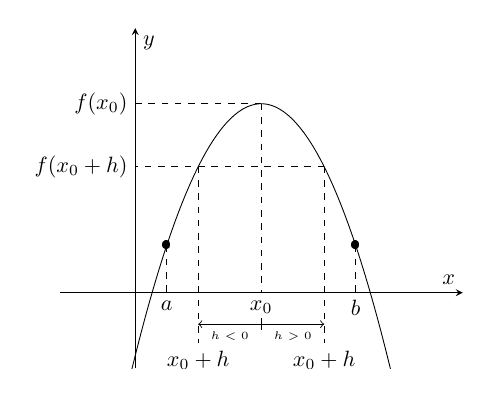
\begin{tikzpicture}[scale = 0.8]
                \begin{axis}[
                    x=1.0cm,y=1.0cm,
                    axis lines=middle,
                    xlabel = $x$,
                    ylabel =$y$,
                    xmin=-1.7,
                    xmax=5.2,
                    ymin=-1.2,
                    ymax=4.2,
                    xtick={-10.0,0.0,...,10.0},
                    ytick={-10.0,0.0,...,10.0},]
                    \draw [samples=100, domain=-1.2:5.2] plot(\x,{-((\x)-2)^2+3});
                    \draw[dashed] (2,3) -- (0,3) node[left]{$f(x_0)$};
                    \draw[dashed] (2,3) -- (2,0) node[below]{$x_0$};
                    \draw[dashed] (3, 2) -- (0,2) node[left]{$f(x_0+h)$}; 
                    \draw[color=white, ultra thick] (-1.2,0)--(-1.7,0);
                    \draw[dashed] (1, 2) -- (1,-0.8) node[below]{$x_0+h$}; 
                    \draw[dashed] (3, 2) -- (3,-0.8) node[below]{$x_0+h$}; 
                    \draw[->] (2,-0.5) --node[below]{\tiny$ h<0$} (1,-0.5);
                    \draw[->] (2,-0.5) --node[below]{\tiny$ h>0$} (3,-0.5);
                    \draw (2,-0.4)--(2,-0.6);
                    \draw[dashed] (0.5, 0.75) -- (0.5,0) node[below]{$a$}; 
                    \draw[dashed] (3.5, 0.75) -- (3.5,0) node[below]{$b$};
                    \node at (0.5, 0.75){\textbullet}; 
                    \node at (3.5, 0.75){\textbullet};
                 \end{axis}
            \end{tikzpicture}
        \end{minipage}}
        \begin{proof}
        Per definizione di punto di massimo relativo
        \[f(x) \leq f(x_0) ~~~~\forall x \in I(x_0)\]
        \[f(x_0+h)\leq f(x_0)\]
        \[f(x_0+h)-f(x_0)\leq 0~~~~ \forall h \in \R\]
        Calcolo i rapporti incrementali da sinistra e da destra:
        \[\mathbf{h>0}~~~~ \frac{f(x_0+h)-f(x_0)}{h}\leq 0\]
        \[\mathbf{h<0}~~~~ \frac{f(x_0+h)-f(x_0)}{h}\geq 0\]
        Per l'inverso del teorema della permanenza del segno:
        \[f'_+(x_0)=\lim_{h\to 0^+}\frac{f(x_0+h)-f(x_0)}{h}\leq 0\]
        \[f'_-(x_0)=\lim_{h\to 0^-}\frac{f(x_0+h)-f(x_0)}{h}\geq 0\]
        Siccome $f(x)$ è derivabile per ipotesi 2, per il criterio di derivabilità
        \[f'_+(x_0)=f'_-(x_0)\]
        Di conseguenza è necessario che \[f'_+(x_0)=f'_-(x_0)=f'(x_0)=0\].
        \end{proof}
        
        \begin{oss}[1]
            Il teorema fornisce una condizione necessaria ma non sufficiente per l'esistenza di un massimo o di un minimo relativo. Non garantisce che se la derivata si annulla allora si presenti un massimo/minimo relativo: potrebbe esserci un flesso a tangente orizzontale.
        \end{oss}
        \begin{oss}[2]
            I punti di massomo e minimo locali non è detto che siano punti stazionari. Lo sono se e solo se sono interni al dominio e la funzione è derivabile. Si possono presentare tuttavia anche agli estremi del dominio o nei punti di non derivabilità.
        \end{oss}

    \subsection{Teorema di Rolle}
        \begin{shadedTheorem}[Rolle]
        Data una funzione $y=f(x)$ definita in un intervallo limitato e chiuso $[a;b]$ tale che \begin{enumerate}
            \item $f(x)$ è continua in $[a;b]$
            \item $f(x)$ è derivabile in $]a;b[$
            \item $f(a)=f(b)$
        \end{enumerate}
        allora esiste almeno un punto $c$ interno all'intervallo per il quale risulta $f'(c)=0$
        \end{shadedTheorem}
        \begin{tabular}{m{0.45\textwidth}m{0.45\textwidth}}
            \textit{Ipotesi} & \textit{Tesi}  \\
            \begin{enumerate}
            \item $f:[a;b] \to \R$
            \item $f(x)$ continua in $[a;b]$
            \item $f(x)$ derivabile in $]a;b[$
            \item $f(a)=f(b)$
        \end{enumerate} & $f'(c)=0$
        \end{tabular}
        
        \begin{proof}
        Dato che per ipotesi $f(x)$ è continua in un intervallo chiuso e limitato $[a;b]$ allora per il teorema di Weistrass $f(x)$ ammette massimo e minimo \textbf{assoluti} in tale intervallo, cioè \[\exists c,d \in [a;b] : m=f(c)\leq f(x)\leq f(d) = M\]
        \begin{figure}
            \centering
            %FIGURA
        \end{figure}
        Possiamo distinguere due casi:
        \begin{enumerate}
            \item $\mathbf{m=M}\to m=f(c)= f(x)= f(d) = M$\\
            Se $m$ e $M$ coincidono vuol dire che $f(x)$ assume sempre lo stesso valore. Dato che $f(x)$ deve essere compresa tra $m$ e $M$\[m\leq f(x) \leq M\]
            ma siccome $m=M$ allora $f(x)=m=M ~~\forall x \in [a;b]$, per cui $f(x)$ è costante. Siccome la derivata di una funzione costante è nulla \[f'(x)=0~~\forall x \in [a;b]\].
            \item $\mathbf{m<M}$, quindi $f(x)$ non è costante ($f(c)\neq f(d)$) e dato che sappiamo che $f(a)=f(b)$ allora \textbf{almeno} uno dei punti $c$ e $d$ deve essere interno all'intervallo $[a;b]$.\\ Supponiamo che $c\in ]a;b[$, quindi che $c$ non sia un estremo. Allora la funzione presenta un punto di minimo assoluto (analog. massimo) all'interno dell'intervallo. Inoltre per ipotesi essa è continua e derivabile in $c$, per cui per il teorema di Fermat $f'(c)=0$.
        \end{enumerate}
        \end{proof}
    \subsubsection{Un'applicazione del teorema di Rolle}
    \begin{ex}
        [Dimostrare che il grafico della funzione $y=x^5+x^3+1$ interseca l'asse $x$ in un solo punto.]
        \begin{proof}
            Consideriamo la funzione $y=x^5+x^3+1$. Siccome è una funzione polinomiale, essa è continua e derivabile su tutto $\R$. Di conseguenza, siccome
            \[\lim_{x\to-\infty}x^5+x^3+1=-\infty\qquad \qquad \lim_{x\to+\infty}x^5+x^3+1=+\infty.\]
            Di conseguenza per il teorema di Bolzano la funzione interseca l'asse $x$ in almeno un punto.

            Supponiamo ora per assurdo che esistano $x_1$ e $x_2$ distinti tali che $f(x_1)=f(x_2)=0$. Allora la funzione soddisferebbe le ipotesi del teorema di Rolle  in $[x_1,x_2]$, per cui dovrebbe esistere un $c\in [x_1,x_2]$ tale che $f'(c)=0$. Calcoliamo quindi $f'(x)=5x^4+3x^2$ e osserviamo che la funzione presenta un punto stazionario in $x=0$. Per il teorema di Rolle esso deve essere un punto di massimo o minimo relativo. Studiamo quindi il segno della derivata prima per classificare il punto stazionario e osserviamo che essa è positiva $\forall x \in \R \setminus \{0\}$. La funzione presenta quindi un flesso a tangente orizzontale e non un punto di massimo/minimo relativo. È quindi falsa la tesi del teorema di Rolle, per cui è falsa l'ipotesi per assurdo, da cui segue la tesi.
        \end{proof}
    \end{ex}
    \subsection{Teorema di Lagrange}\label{subsection: teorema di Lagrange}
        \begin{shadedTheorem}[Lagrange]
        Data una funzione $y=f(x)$ definita in un intervallo limitato e chiuso $[a;b]$ tale che \begin{enumerate}
            \item $f(x)$ è continua in $[a;b]$
            \item $f(x)$ è derivabile in $]a;b[$
        \end{enumerate}
        allora esiste almeno un punto $c$ interno all'intervallo per il quale vale la relazione \[\frac{f(b)-f(a)}{b-a}=f'(c)\]
        \end{shadedTheorem}
        \begin{tabular}{m{0.45\textwidth}m{0.45\textwidth}}
            \textit{Ipotesi} & \textit{Tesi}  \\
            \begin{enumerate}
            \item $f:[a;b] \to \R$
            \item $f(x)$ continua in $[a;b]$
            \item $f(x)$ derivabile in $]a;b[$
        \end{enumerate} & $\exists c \in~~]a;b[ ~~:~~ \dfrac{f(b)-f(a)}{b-a}=f'(c)$
        \end{tabular}
        \begin{proof}
            Definiamo $h(x):= f(x)-\dfrac{f(b)-f(a)}{b-a}(x-a)$. Osserviamo che \[h(a)=f(a)\] e \[h(b)=f(b)-\dfrac{f(b)-f(a)}{b-a}(b-a)= f(a),\]
            per cui essa soddisfa le ipotesi del teorema di Rolle, di conseguenza esiste un punto $c$ tale che $h'(c)=0$. Osserviamo che
            \[h'(x)=f'(x)-\dfrac{f(b)-f(a)}{b-a}, \]
            quindi siccome $h(c)=0$
            \[f'(c)=\dfrac{f(b)-f(a)}{b-a}.\]
        \end{proof}
        \subsection{Conseguenze del teorema di Lagrange}
        \subsubsection{Funzioni con derivata nulla}
            \begin{shadedTheorem}[Derivata nulla]
                Se $f(x)$ è una funzione continua in un intervallo $[a;b]$, derivabile in $]a;b[$ e la sua derivata è nulla per ogni punto interno all'intervallo, allora $f(x)$ è costante in tutto $[a;b]$
            \end{shadedTheorem}
            \begin{tabular}{m{0.45\textwidth}m{0.45\textwidth}}
                \textit{Ipotesi} & \textit{Tesi}  \\ 
                \begin{enumerate}
                \item $f:[a;b] \to \R$
                \item $f(x)$ continua in $[a;b]$
                \item $f(x)$ derivabile in $]a;b[$
                \item $f'(x)=0~~\forall x \in [a;b]$
        \end{enumerate} & $f(x)=k ~~ \forall x \in [a;b]$
           \end{tabular}
           
        \subsubsection{Funzioni con derivate uguali}
            \begin{shadedTheorem}[Differenza costante]
                Se $f(x)$ e $g(x)$ sono due funzioni continue nell'intervallo $[a;b]$, derivabili in $]a;b[$ e tali che $f'(x)=g'(x)~~\forall x \in ]a;b[$, allora esse differiscono per una costante.
            \end{shadedTheorem}
            \begin{tabular}{m{0.45\textwidth}m{0.45\textwidth}}
            \textit{Ipotesi} & \textit{Tesi}\\
            \begin{enumerate}
                \item $f:[a;b] \to \R$, $g: [a;b] \to \R$
                \item $f(x)$ continua in $[a;b]$
                \item $f(x)$ derivabile in $]a;b[$
                \item $g(x)$ continua in $[a;b]$
                \item $g(x)$ derivabile in $]a;b[$
                \item $f'(x)=g'(x) ~~ \forall x \in [a;b]$
        \end{enumerate} & $f(x)-g(x) = k ~~ \forall x \in [a;b]$
           \end{tabular}
        \subsubsection{Monotonia di funzioni derivabili}
            \begin{shadedTheorem}[Monotonia di funzioni derivabili]
                Data una funzione $y=f(x)$, continua in un intervallo $[a;b]$ e derivabile nell'intervallo $]a;b[$: \begin{enumerate}
                    \item se $f'(x)>0 ~~\forall x \in ]a;b[$, allora $f(x)$ è crescente in $]a;b[$
                    \item se $f'(x)<0 ~~\forall x \in ]a;b[$, allora $f(x)$ è decrescente in $]a;b[$
                \end{enumerate} 
            \end{shadedTheorem}
            \begin{shadedTheorem}[Inverso della monotonia di funzioni derivabili]
                Data una funzione $y=f(x)$, continua in un intervallo $[a;b]$ e derivabile nell'intervallo $]a;b[$: \begin{enumerate}
                    \item se $f(x)$ è crescente in $]a;b[$, allora $f'(x)\geq0 ~~\forall x \in ]a;b[$
                    \item se $f(x)$ è decrescente in $]a;b[$, allora $f'(x)\leq0 ~~\forall x \in ]a;b[$
                \end{enumerate} 
            \end{shadedTheorem}

        \subsection{Teorema di Cauchy}
        \begin{shadedTheorem}[Cauchy]
        Siano $y=f(x)$ e $y=g(x)$ due funzioni tali che 
        \begin{enumerate}
            \item $f(x)$ e $g(x)$ sono continue in $[a;b]$
            \item $f(x)$ e $g(x)$ sono è derivabili in $]a;b[$
            \item $g'(x)\neq 0 ~~ \forall x \in ]a;b[$ 
        \end{enumerate}
        allora esiste almeno un punto $c$ interno all'intervallo per il quale vale la relazione \[\frac{f(b)-f(a)}{g(b)-g(a)}=\frac{f'(c)}{g'(c)}\]
        \end{shadedTheorem}
        \begin{tabular}{m{0.45\textwidth}m{0.45\textwidth}}
            \textit{Ipotesi} & \textit{Tesi}  \\
            \begin{enumerate}
            \item $f:[a;b] \to \R$, $g: [a;b] \to \R$
            \item $f(x)$ continua in $[a;b]$
            \item $f(x)$ derivabile in $]a;b[$
            \item $g(x)$ continua in $[a;b]$
            \item $g(x)$ derivabile in $]a;b[$
            \item $g'(x)\neq 0 ~~ \forall x \in ]a;b[$
        \end{enumerate} & $\exists c \in~~]a;b[ ~~:~~ \dfrac{f(b)-f(a)}{g(b)-g(a)}=\dfrac{f'(c)}{g'(c)}$
        \end{tabular}

    \subsection{Teorema di De l'Hôpital}\label{subsection: de l'Hopital}
    \textbf{N.B.:} Applicabile per la risoluzione delle forme di indecisione $\left[\frac{0}{0}\right]$ o $\left[\frac{\infty}{\infty}\right]$
        \begin{shadedTheorem}[De l'Hôpital]
            Date due funzioni $f(x)$ e $g(x)$ definite nell'intorno $I$ di un punto $x_0\in \overline{\R}$, se
            \begin{enumerate}
                \item $f(x)$ e $g(x)$ sono continue in $x_0$ e $f(x_0)=g(x_0)=0$ (o $\infty$)
                \item $f(x)$ e $g(x)$ sono derivabili in $I(x_0)-\{x_0\}$ 
                \item $g'(x)\neq 0$ in $I(x_0)-\{x_0\}$
                \item esiste $\lim_{x\to x_0}\frac{f'(x)}{g'(x)}$
            \end{enumerate}
            Allora esiste anche $\lim_{x\to x_0}    \frac{f(x)}{g(x)}$ e risulta:
            \[\lim_{x\to x_0}\frac{f(x)}{g(x)}\underset{\mathrm{H}}{=}\lim_{x\to x_0}\frac{f'(x)}{g'(x)}\]
        \end{shadedTheorem}
        \begin{tabular}{m{0.55\textwidth}m{0.35\textwidth}}
            \textit{Ipotesi} & \textit{Tesi}  \\
            \begin{enumerate}
                \item $f: I(x_0)\to \R$
                \item $g: I(x_0)\to \R$
                \item $f(x)$ e $g(x)$ continue in $x_0$ e $f(x_0)=g(x_0)=0$ (o $\infty$)
                \item $f(x)$ e $g(x)$ derivabili in $I(x_0)-\{x_0\}$ 
                \item $g'(x)\neq 0 ~~\forall~ x \in I(x_0)-\{x_0\}$
                \item $\exists \lim_{x\to x_0}\frac{f'(x)}{g'(x)}$
            \end{enumerate} & \[\lim_{x\to x_0}\frac{f(x)}{g(x)}\underset{\mathrm{H}}{=}\lim_{x\to x_0}\frac{f'(x)}{g'(x)}\]
        \end{tabular}
    \begin{ex}[Calcolare i seguenti limiti applicando il teorema di de l'Hôpital
        \begin{tasks}(3)
            \task $\lim_{x\to 1}\frac{x^2-1}{\ln x}$
            \task $\lim_{x\to +\infty}\frac{\ln(e^x+1)}{x}$
            \task $\lim_{x\to +\infty}\frac{\sin x}{x}$
        \end{tasks}
        ]
        \begin{tasks}
            \task \[\lim_{x\to 1}\frac{x^2-1}{\ln x}=\left[ \frac{0}{0} \right]\overset{LN}{\underset{H}=}\lim_{x\to 1}\frac{2x}{\frac{1}{x}}=\left[ \frac{2}{1} \right]=2\]
            \task \[\lim_{x\to +\infty}\frac{\ln(e^x+1)}{x}=\left[ \frac{\infty}{\infty} \right]\overset{LN}{\underset{H}=}\lim_{x\to +\infty}\frac{\frac{e^x}{e^x+1}}{1}=\lim_{x\to +\infty}\frac{e^x}{e^x+1}=\left[ \frac{\infty}{\infty} \right]\overset{LN}{\underset{H}=} \lim_{x\to+\infty}\frac{\cancel{e^x}}{\cancel{e^x}}=1\]
            Il teorema di de l'Hôpital può essere applicato più volte a condizione che ogni volte siano verificate le ipotesi.
            \task \[\lim_{x\to +\infty}\frac{\sin x}{x}= \left[ \frac{0}{0} \right]\overset{LN}{\underset{H}=}\lim_{x\to 0}\frac{\cos x}{1}=1\]
            Questa è una valida dimostrazione del limite notevole, tuttavia la prova geometrica presentata precedentemente è maggiormente elegante e quindi è da preferirsi.
        \end{tasks}
        
    \end{ex}
\section{Studio della derivata}
Grazie ai teoremi che abbiamo appena enunciato possiamo sfruttare la derivata per ottenere importanti informazioni sul grafico della funzione di partenza. Infatti per il corollario di Lagrange (Monotonia di funzioni derivabili), sappiamo che il segno della derivata è direttamente correlato alla monotonia della funzione. Inoltre, ricordando la definizione di derivata come coefficiente angolare della retta tangente, abbiamo che i punti in cui essa si annulla sono punti in cui la retta tangente al grafico è parallela all'asse delle ascisse. Di conseguenza definiamo questi come punti stazionari. Essi sono classificati in tre categorie: 
\subsection{Punti di massimo relativo}
Si parla di punto di massimo relativo quando la derivata di una funzione è positiva in un intorno sinistro del punto stazionario e negativa in un intorno destro del punto stazionario.
\subsection{Punti di minimo relativo}
Si parla di punto di minimo relativo quando la derivata di una funzione è negativa in un intorno sinistro del punto stazionario e positiva in un intorno destro del punto stazionario.
\subsection{Punti di flesso a tangente orizzontale}
Si parla di punto di flesso a tangente orizzontale quando in un intorno completo del punto stazionario la derivata mantiene segno costante, per cui la funzione è sempre crescente o sempre decrescente.
\begin{figure}[ht]
    \centering
    \begin{subfigure}{0.24\textwidth}
        \centering
        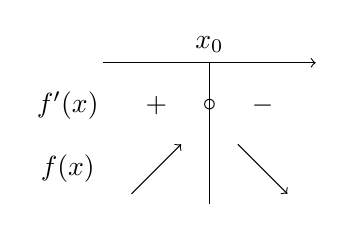
\begin{tikzpicture}[scale=0.9]
            \draw[->](0,0)--(3,0);
            \draw(1.5,0) node[above]{$x_0$}--(1.5,-2);
            \node at (-0.50, -0.60){$f'(x)$};
            \node at (-0.50, -1.50){$f(x)$};
            \node at (0.75,-0.60) {$+$};
            \node at (2.25,-0.60) {$-$};
            \node at (1.5, -0.60) {$\circ$};
            \draw[->] (0.4,-1.85)--(1.1,-1.15); %+ sx
            \draw[->] (1.9,-1.15)--(2.6,-1.85); %- dx
        \end{tikzpicture}
        \caption{Massimo relativo}
    \end{subfigure}
    \begin{subfigure}{0.24\textwidth}
        \centering
        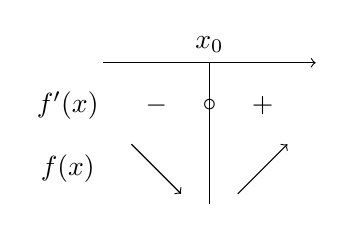
\begin{tikzpicture}[scale=0.9]
            \draw[->](0,0)--(3,0);
            \draw(1.5,0) node[above]{$x_0$}--(1.5,-2);
            \node at (-0.50, -0.60){$f'(x)$};
            \node at (-0.50, -1.50){$f(x)$};
            \node at (0.75,-0.60) {$-$};
            \node at (2.25,-0.60) {$+$};
            \node at (1.5, -0.60) {$\circ$};
            \draw[->] (0.4,-1.15)--(1.1,-1.85); %- sx
            \draw[->] (1.9,-1.85)--(2.6,-1.15); %+ dx
        \end{tikzpicture}
        \caption{Minimo relativo}
    \end{subfigure}
    \begin{subfigure}{0.24\textwidth}
        \centering
        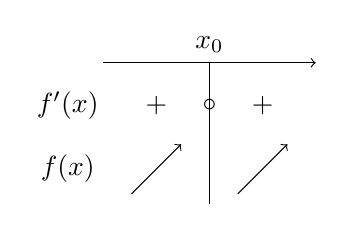
\begin{tikzpicture}[scale=0.9]
            \draw[->](0,0)--(3,0);
            \draw(1.5,0) node[above]{$x_0$}--(1.5,-2);
            \node at (-0.50, -0.60){$f'(x)$};
            \node at (-0.50, -1.50){$f(x)$};
            \node at (0.75,-0.60) {$+$};
            \node at (2.25,-0.60) {$+$};
            \node at (1.5, -0.60) {$\circ$};
            %\draw[->] (0.4,-1.15)--(1.1,-1.85); %- sx
            \draw[->] (0.4,-1.85)--(1.1,-1.15); %+ sx
            %\draw[->] (1.9,-1.15)--(2.6,-1.85); %- dx
            \draw[->] (1.9,-1.85)--(2.6,-1.15); %+ dx
        \end{tikzpicture}
        \caption{Flesso ascendente}
    \end{subfigure}
    \begin{subfigure}{0.24\textwidth}
        \centering
        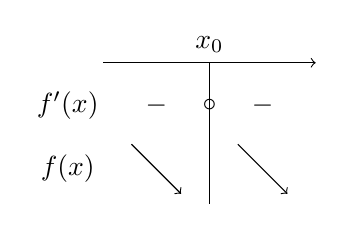
\begin{tikzpicture}[scale=0.9]
            \draw[->](0,0)--(3,0);
            \draw(1.5,0) node[above]{$x_0$}--(1.5,-2);
            \node at (-0.50, -0.60){$f'(x)$};
            \node at (-0.50, -1.50){$f(x)$};
            \node at (0.75,-0.60) {$-$};
            \node at (2.25,-0.60) {$-$};
            \node at (1.5, -0.60) {$\circ$};
            \draw[->] (0.4,-1.15)--(1.1,-1.85); %- sx
            \draw[->] (1.9,-1.15)--(2.6,-1.85); %- dx
        \end{tikzpicture}
        \caption{Flesso discendente}
    \end{subfigure}
    \caption{}
\end{figure}
\section{Derivata seconda e flessi a tangente obliqua}
Lo studio della derivata seconda permette di ottenere informazioni sulla concavità e sulla convessità di una convessità di una funzione. La derivata seconda si calcola semplicemente derivando la derivata prima. Quando la derivata seconda è positiva, la funzione di partenza è convessa (presenta una concavità verso l'alto); quando la derivata seconda è negativa, la funzione è concava (presenta una concavità verso il basso).

Quando la derivata seconda si annulla la funzione può presentare un punto di flesso, ovvero un punto in cui la dunzione inverte la sua concavità (altrimenti può trattarsi di un punto stazionario). Se il flesso non è a tangente orizzontale si dice \textbf{a tangente obliqua}. La retta tangente può essere individuata applicando la formula per la retta tangente al grafico di una funzione in un punto.
\section{Problemi di ottimizzazione}
Si dice problema di ottimizzazione un problema nel quale si cerca di massimizzare o minimizzare una grandezza, ad esempio il volume di un solido, l'area di una superficie, \dots

Vediamo un esempio di problema di ottimizzazione:
\begin{ex}
    [Nella figura è rappresentato il grafico della funzione \[y=\frac{1}{ax^2+bx+c}\] simmetrica rispetto all'asse $y$. 
    \begin{itemize}
        \item Trovare $a,b,c$
    \end{itemize}
    La retta $x=k$ e la sua simmetrica $x=-k$ determinano il rettangolo $PP'Q'Q$:
    \begin{itemize}
        \item trovare per quale valore di $k$ l'area $PP'Q'Q$ è massima.
    \end{itemize}
    ]
    \begin{center}
        \begin{tikzpicture}[scale=0.9,line cap=round,line join=round,>=triangle 45,x=1.0cm,y=1.0cm]
            \begin{axis}[
            x=1.5cm,y=1.5cm,
            axis lines=middle,
            xmin=-2.5,
            xmax=2.5,
            ymin=-0.7,
            ymax=1.6,
            xtick={-2.0,0,...,2.0},
            ytick={0.0,1.0,...,1.0},]
            \clip(-2.5,-0.8) rectangle (2.5,1.7);
            \fill[line width=1.5pt,color=black,fill=black,fill opacity=0.10000000149011612] (1.,0.5) -- (-1.,0.5) -- (-1.,0.) -- (1.,0.) -- cycle;
            \draw[line width=1.5pt,color=black,smooth,samples=100,domain=-2.5:2.5] plot(\x,{1/(1+(\x)^(2))});
            \draw [line width=1.5pt,color=black] (1.,0.5)-- (-1.,0.5);
            \draw [line width=1.5pt,color=black] (-1.,0.5)-- (-1.,0.);
            \draw [line width=1.5pt,color=black] (-1.,0.)-- (1.,0.);
            \draw [line width=1.5pt,color=black] (1.,0.)-- (1.,0.5);
            \draw [line width=1.pt,dash pattern=on 4pt off 4pt,color=black] (1.,-0.8) -- (1.,1.7);
            \draw [line width=1.pt,dash pattern=on 4pt off 4pt,color=black] (-1.,-0.8) -- (-1.,1.7);
            \draw (-0.9586267284296891,-0.06868827636263657) node[anchor=north west] {$x=-k$};
            \draw (1.0391893112679038,-0.10638291862108168) node[anchor=north west] {$x=k$};
            \begin{scriptsize}
            \draw [fill=black] (2.,0.2) circle (2.5pt);
            \draw[color=black] (2,0.5281435593960777) node {$A\left(2,\frac{1}{5}\right)$};
            \draw [fill=black] (0.,1.) circle (2.5pt);
            \draw[color=black] (0.08425837405396008,1.2317768815537196) node {$B(0,1)$};
            \draw [fill=black] (1.,0.5) circle (2.5pt);
            \draw[color=black] (1.0894488342791642,0.7291816514411182) node {$P$};
            \draw [fill=black] (-1.,0.5) circle (2.5pt);
            \draw[color=black] (-0.8706725631599838,0.7291816514411182) node {$P'$};
            \draw [fill=black] (1.,0.) circle (2.5pt);
            \draw[color=black] (1.0894488342791642,0.2265864213285168) node {$Q$};
            \draw [fill=black] (-1.,0.) circle (2.5pt);
            \draw[color=black] (-0.8706725631599838,0.2265864213285168) node {$Q'$};
            \end{scriptsize}
            \end{axis}
            \end{tikzpicture}
        \end{center}
\begin{itemize}
    \item Osserviamo che la funzione è pari, per cui si deve avere $b=0$. Per cui la funzione è del tipo $y=\frac{1}{ax^2+c}$. Imponiamo ora le condizioni di passaggio per i due punti $A\left(2,\frac{1}{5}\right)$ e $B(0,1)$
    \[\begin{array}{r}
        A\left(2,\frac{1}{5}\right)\\
        B(0,1)
    \end{array} \quad\begin{cases}
        \frac{1}{5}=\frac{1}{4a+c}\\
        1=\frac{1}{c}
    \end{cases}\qquad
    \begin{cases}
        \frac{1}{5}=\frac{1}{4a+1}\\
        c=1
    \end{cases}
    \begin{cases}
        {5}={4a+1}\\
        c=1
    \end{cases}
    \]
    Per cui otteniamo $a=1$ e $c=1$. Di conseguenza la funzione cercata sarà
    \[y=\frac{1}{x^2+1}.\]
    Siccome $P\in f$, abbiamo che $P\left(k, \frac{1}{k^2+1}\right)$. Per simmetria troviamo $P'\left(-k, \frac{1}{k^2+1}\right)$. \\Analogamente troviamo $Q(k,0)$ e $ Q'(-k,0)$. Per cui l'area del rettangolo in funzione di $k$ è 
    \[b=2\overline{OQ}=2k\qquad \qquad h=\overline{PQ}=\frac{1}{k^2+1}\]
    \[A(k)=2k\cdot \frac{1}{k^2+1}=\frac{2k}{k^2+1}\]
    Ora dobbiamo trovare per quale valore di $k$ la funzione area è massima, per cui quando la sua derivata si annulla:
    \[A'(k)=\frac{2(k^2+1)-2k(2k)}{(k^2+1)^2}=\frac{2k^2+2-4k^2}{(k^2+1)^2}=\frac{-2k^2+2}{(k^2+1)^2}\]
    Osserviamo che la derivata si annulla per $k=1$ e $k=-1$. Dobbiamo trovare per quale dei due valori di $k$ l'area è massima. Studiamo quindi il segno della derivata: 
    \begin{center}
        \begin{tikzpicture}
            \node at (-1,0.4) [anchor=west]{$N: -2k^2+2>0$};
            \node at (-1,-0.4)[anchor=west]{$D: (k^2+1)^2>0$};
            \node at (2.75,0.4)[anchor=west]{$k^2<1$};
            \node at (2.75,-0.4)[anchor=west]{$\forall \, x \in \R$};
            \node at (4.5,0.4)[anchor=west]{$-1<k<1$};
            \draw[->] (7.5,1)--(11.5,1);
            \draw (8.75,1)node [above]{$-1$}--(8.75,-1);
            \draw (10.25,1) node [above]{$1$}--(10.25,-1);
            \draw[color=red, dashed] (7.5, 0.4)--(8.75,0.4) node {$\circ$};
            \draw[color=red] (8.75, 0.4)--(10.25,0.4) node {$\circ$};
            \draw[color=red, dashed] (10.25, 0.4)--(11.5,0.4);
            \draw[color=red] (7.5, -0.4)--(11.5,-0.4);
            \node [color=red]at (8.125,-0.8){$\searrow$};
            \node [color=red]at (9.5,-0.8){$\nearrow$};
            \node [color=red]at (11,-0.8){$\searrow$};
        \end{tikzpicture}
    \end{center}
    La funzione presenta quindi un punto di massimo per $k=1$.
\end{itemize}
\end{ex}

\chapter{Studio di funzione completo}
Proponiamo qui una traccia per studiare una funzione al fine di produrre un grafico probabile. Non è necessario né svolgere tutti i punti né svolgerli in ordine. Si consiglia di iniziare da subito a tracciare il grafico e di aggiornarlo man mano in mado di verificare progressivamente tutte le parti dello studio di funzione. Di seguito si riportano alcuni esempi.
\section{Traccia per lo studio di funzione completo}
    \subsection{Classificazione}
    \begin{tabular}{|c|c|c|c|}
        \hline
        \multirow{2}{4em}{Funzione} & algebrica\ & razionale & intera\\ \cline{2-4}
         & trascendente & irrazionale & fratta \\ \hline
    \end{tabular}
    \subsection{Dominio}
    \begin{itemize}
        \item Polinomiale : $\R$
        \item Fratte: denominatore $\neq 0$
        \item Irrazionali pari: radicando$\geq0$
        \item Irrazionali dispari: $\R$
        \item Logaritmi: argomento$>0$
        \item Esponenziali: $\R$
        \item Seno, coseno, arcotangente, arcocotangente: $\R$
        \item Tangente: $\R \setminus \{\frac{\pi}{2}+k\pi\}\text{, con } k\in\Z$
        \item Cotangente: $\R \setminus \{k\pi\}\text{, con } k\in\Z$
        \item Arcoseno, arcocoseno: $[-1;1]$
    \end{itemize}
    \subsection{Simmetrie}
    \textbf{CN:} $\forall x \in D, -x \in D$
    \begin{itemize}
        \item pari se $f(-x)=f(x)$
        \item dispari se $f(-x)=-f(x)$
    \end{itemize}
    \subsection{Intersezioni con gli assi cartesiani}
    \[f(x) \cap \text{asse~}x : \left\{\begin{array}{l}
         y=f(x)  \\
         y=0 
    \end{array}\right.~~~~~~~~ 
    f(x) \cap \text{asse~}y : \left\{\begin{array}{l}
         y=f(x)  \\
         x=0 
    \end{array}\right.\] 
    \subsection{Studio del segno}
    Risolvere la disequazione $f(x)>0$
    \subsection{Limiti, asintoti e discontinuità}
    \begin{tabular}{|m{0.3\textwidth}|m{0.6\textwidth}|}
        \hline
        Asintoto verticale&  \[\lim_{x\rightarrow x_0} f(x) = \infty\] \\\hline
        Asintoto orizzontale & \[\lim_{x\rightarrow \infty} f(x) = l\]\\ \hline
        Asintoto obliquo & \[\textnormal{CN: }\lim_{x\rightarrow\infty}f(x) = \infty\]
        \[m=\lim_{x\rightarrow\infty}\frac{f(x)}{x}\]
        \[q=\lim_{x\rightarrow\infty}f(x)-mx\] \\ \hline
    \end{tabular}\\
    \\
    \textbf{NB.:} Una funzione può avere anche infiniti asintoti verticali, ma al massimo due tra asintoti orizzontali e asintoti obliqui (uno destro e uno sinistro).\\    \begin{tabular}{|m{0.3\textwidth}|m{0.6\textwidth}|}
        \hline
        Prima specie &  \[\lim_{x\rightarrow x_0^-}f(x)=l_1~~~~\lim_{x\rightarrow x_0^+}f(x)=l_2\] \[l_1\neq l_2~~~~salto=|l_1-l_2|\]\\ \hline
        Seconda specie &  \[\lim_{x\rightarrow x_0^\pm}f(x)=\infty ~~~~\lor~~~~ \lim_{x\rightarrow x_0^\pm}f(x)=\nexists\] \\\hline
        Terza specie & \[\lim_{x\rightarrow x_0^-}f(x)=\lim_{x\rightarrow x_0^+}f(x)=l\]\[f(x_0)\neq l ~~~~ \lor ~~~~ f(x_0)=\nexists\]\\ \hline
    \end{tabular}
    \subsection{Derivata prima}
    Le soluzioni dell'equazione \[f'(x) = 0\] identificano la presenza di \begin{itemize}
        \item massimi relativi
        \item minimi relativi
        \item flessi a tangente orizzontale
    \end{itemize}
    Per distinguerli è necessario studiare il segno della derivata:
    \begin{figure}[ht]
        \centering
        \begin{subfigure}{0.24\textwidth}
            \centering
            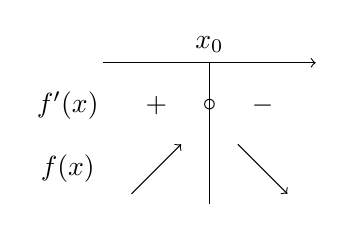
\begin{tikzpicture}[scale=0.9]
                \draw[->](0,0)--(3,0);
                \draw(1.5,0) node[above]{$x_0$}--(1.5,-2);
                \node at (-0.50, -0.60){$f'(x)$};
                \node at (-0.50, -1.50){$f(x)$};
                \node at (0.75,-0.60) {$+$};
                \node at (2.25,-0.60) {$-$};
                \node at (1.5, -0.60) {$\circ$};
                \draw[->] (0.4,-1.85)--(1.1,-1.15); %+ sx
                \draw[->] (1.9,-1.15)--(2.6,-1.85); %- dx
            \end{tikzpicture}
            \caption{Massimo relativo}
        \end{subfigure}
        \begin{subfigure}{0.24\textwidth}
            \centering
            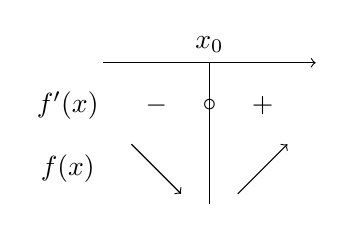
\begin{tikzpicture}[scale=0.9]
                \draw[->](0,0)--(3,0);
                \draw(1.5,0) node[above]{$x_0$}--(1.5,-2);
                \node at (-0.50, -0.60){$f'(x)$};
                \node at (-0.50, -1.50){$f(x)$};
                \node at (0.75,-0.60) {$-$};
                \node at (2.25,-0.60) {$+$};
                \node at (1.5, -0.60) {$\circ$};
                \draw[->] (0.4,-1.15)--(1.1,-1.85); %- sx
                \draw[->] (1.9,-1.85)--(2.6,-1.15); %+ dx
            \end{tikzpicture}
            \caption{Minimo relativo}
        \end{subfigure}
        \begin{subfigure}{0.24\textwidth}
            \centering
            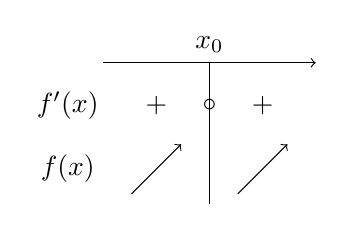
\begin{tikzpicture}[scale=0.9]
                \draw[->](0,0)--(3,0);
                \draw(1.5,0) node[above]{$x_0$}--(1.5,-2);
                \node at (-0.50, -0.60){$f'(x)$};
                \node at (-0.50, -1.50){$f(x)$};
                \node at (0.75,-0.60) {$+$};
                \node at (2.25,-0.60) {$+$};
                \node at (1.5, -0.60) {$\circ$};
                %\draw[->] (0.4,-1.15)--(1.1,-1.85); %- sx
                \draw[->] (0.4,-1.85)--(1.1,-1.15); %+ sx
                %\draw[->] (1.9,-1.15)--(2.6,-1.85); %- dx
                \draw[->] (1.9,-1.85)--(2.6,-1.15); %+ dx
            \end{tikzpicture}
            \caption{Flesso ascendente}
        \end{subfigure}
        \begin{subfigure}{0.24\textwidth}
            \centering
            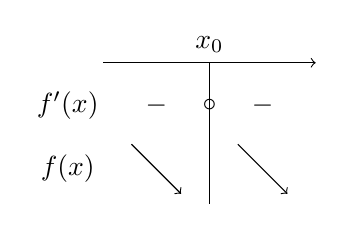
\begin{tikzpicture}[scale=0.9]
                \draw[->](0,0)--(3,0);
                \draw(1.5,0) node[above]{$x_0$}--(1.5,-2);
                \node at (-0.50, -0.60){$f'(x)$};
                \node at (-0.50, -1.50){$f(x)$};
                \node at (0.75,-0.60) {$-$};
                \node at (2.25,-0.60) {$-$};
                \node at (1.5, -0.60) {$\circ$};
                \draw[->] (0.4,-1.15)--(1.1,-1.85); %- sx
                \draw[->] (1.9,-1.15)--(2.6,-1.85); %- dx
            \end{tikzpicture}
            \caption{Flesso discendente}
        \end{subfigure}
        \caption{}
    \end{figure}
    Lo studio della derivata prima fornisce anche informazioni circa la monotonia della funzione.
    \subsection{Derivata seconda}
    Le soluzioni dell'equazione \[f''(x)=0\] permettono di identificare i punti di flesso. A differenza della derivata prima permette di ottenere informazioni circa la presenza di flessi a tangente obliqua, per cui è necessario escludere tutte le soluzioni già analizzate in precedenza. 
    La derivata seconda fornisce inoltre informazioni circa la concavità della funzione: verso l'alto quando la derivata seconda è positiva e verso il basso quando la derivata seconda è negativa. La funzione inverte la propria concavità in corrispondenza dei punti di flesso.
    \subsection{Estremi globali}
    In conclusione è opportuno elencare i punti di estremo globali, da ricercarsi tra gli estremi del dominio, i punti stazionari e i punti di non derivabilità.

\section{Esempi}
    \begin{ex}[Studiare la funzione $ y=\frac{x^2}{x-1}$.]
        \begin{enumerate}
            \item \textbf{Classificazione:} funzione algebrica razionale fratta;
            \item \textbf{Dominio:} $\dom f=\;]-\infty;1[\ \cup \ ]1;+\infty[$ 
            \item \textbf{Simmetrie:} il dominio non è simmetrico, per cui la condizione necessaria non è rispettata, di conseguenza la funzione non è né pari né dispari.
            \item \textbf{Intersezioni con gli assi:} è consigliabile partire dalle intersezioni con l'asse $x$, perchè potremmo trovare anche l'unica intersezione con l'asse $y$ nel caso la funzione passi per l'origine.
            \[f(x)=0\ \ \Harr \ \ x^2=0\ \ \Harr \ \ x=0.\]
            La funzione passa appunto per l'origine $O(0,0)$, quindi non ci serve calcolare anche l'intersezione con l'asse $y$.
            \item \textbf{Segno:} $f(x)>0$
            \begin{center}
                \begin{tikzpicture}
                    \node at (1,0.4) [anchor=west]{$N: x^2>0$};
                    \node at (1,-0.4)[anchor=west]{$D: (x-1)>0$};
                    \node at (1,-1.2)[anchor=west]{$\dom f: x\neq 1$};
                    \node at (5,0.4)[anchor=west]{$x\neq 0$};
                    \node at (5,-0.4)[anchor=west]{$x>1$};
                    \draw[->] (7.5,1)--(11.5,1);
                    \draw (8.75,1)node [above]{$0$}--(8.75,-2);
                    \draw (10.25,1) node [above]{$1$}--(10.25,-2);
                    \draw[color=red, dashed] (7.5, -0.4)--(10.25,-0.4) node {$\circ$};
                    %\draw[color=red] (8.75, 0.4)--(10.25,0.4) node {$\circ$};
                    \node [color=red] at (8.75,0.4){$\circ$};
                    \draw [color=red] (10.25, -0.4)--(11.5,-0.4);
                    \draw [color=red] (7.5, 0.4)--(11.5,0.4);
                    \draw [color=red] (7.5, -1.2)--(11.5,-1.2);
                    \node [color=red] at (10.25,-1.2){$\nexists$};
                    \node [color=red]at (8.125,-1.8){$-$};
                    \node [color=red]at (9.5,-1.8){$-$};
                    \node [color=red]at (11,-1.8){$+$};
                \end{tikzpicture}
            \end{center}
            \item \textbf{Limiti, asintoti e discontinuità:} Dobbiamo calcolare i limiti agli estremi del dominio:
            \[\lim_{x\to-\infty}\frac{\boxed{x^{\cancel{2}}}}{\cancel{\boxed{x}}-1}=\left[ \frac{\infty}{\infty} \right]\overset{FI}{=}-\infty \qquad \qquad \lim_{x\to+\infty}\frac{\boxed{x^{\cancel{2}}}}{\cancel{\boxed{x}}-1}=\left[ \frac{\infty}{\infty} \right]\overset{FI}{=}+\infty\]
            È verificata la condizione necessaria per la ricerca dell'asintoto obliquo, per cui procediamo con la ricerca dello stesso:
            \[m=\lim_{x\to\infty}\frac{{x^{{2}}}}{x({{x}}-1)}=\left[ \frac{\infty}{\infty} \right]\overset{FI}{=}\lim_{x\to\infty}\frac{x^2}{x^2-1}=1\]
            \[q=\lim_{x\to \infty}\left(\frac{x^2}{x-1}-x\right)=\lim_{x\to\infty}\frac{x^2-x^2+x}{x-1}=\left[ \frac{\infty}{\infty} \right]\overset{FI}{=}1.\]
            Per cui la funzione ha un asintoto obliquo (destro e sinistro) alla retta $y=x+1$
            \[\lim_{x\to1^-}\frac{x^2}{x-1}=\left[ \frac{1}{0^-} \right]=-\infty\qquad \qquad \lim_{x\to1^+}\frac{x^2}{x-1}=\left[ \frac{1}{0^+} \right]=+\infty\]
            La funzione presenta quindi una discontinuità di seconda specie in $x=1$.
            \item \textbf{Derivata prima:} Calcoliamo la derivata prima della funzione:
            \[f'(x) = \frac{2x(x-1)-x^2(1)}{(x-1)^2}=\frac{2x^2-2x-x^2}{(x-1)^2}=\frac{x^2-2x}{(x-1)^2}=\frac{x(x-2)}{(x-1)^2}\]
            e il suo dominio, che va confrontato con il dominio della funzione per verificare l'eventuale presenza di punti di non derivabilità:
            \[\dom f'= \ ]-\infty,1[\ \cup \ ]1,+\infty[\ = \dom f\]
            la funzione è quindi derivabile su tutto il suo dominio.

            Individuiamo ora i punti stazionari
            \[f'(x)=0\ \ \Harr \ \ \frac{x(x-2)}{(x-1)^2}=0\ \ \Harr \ \ x=0\lor x=2\]
            e studiamo il segno della derivata per classificarli attraverso lo studio della monotonia della funzione: $f'(x)>0$
            \begin{center}
                \begin{tikzpicture}
                    \node at (0,0.4) [anchor=west]{$N: x(x-2)>0$};
                    \node at (0,-0.4)[anchor=west]{$D: (x-1)^2>0$};
                    \node at (0,-1.2)[anchor=west]{$\dom f': x\neq 1$};
                    \node at (4,0.4)[anchor=west]{$x<0\lor x>2$};
                    \node at (4,-0.4)[anchor=west]{$x>1$};
                    \draw[->] (7.5,1)--(13.0,1);
                    \draw (8.75,1)node [above]{$0$}--(8.75,-2);
                    \draw (10.25,1) node [above]{$1$}--(10.25,-2);
                    \draw (11.75,1)node [above]{$2$}--(11.75,-2);
                    \draw[color=red] (7.5, -0.4)--(13,-0.4);
                    \node [color=red] at (10.25,-0.4){$\circ$};
                    \draw[color=red] (7.5, 0.4)--(8.75,0.4) node {$\circ$};
                    \draw [color=red, dashed] (8.75, 0.4)--(11.75,0.4) node {$\circ$}; 
                    \draw[color=red] (11.75, 0.4)--(13,0.4);
                    \draw[color=red] (7.5, -1.2)--(13,-1.2);
                    \node [color=red] at (10.25,-1.2){$\nexists$};
                    \node [color=red]at (8.125,-1.8){$\nearrow$};
                    \node [color=red]at (9.5,-1.8){$\searrow$};
                    \node [color=red]at (11,-1.8){$\searrow$};
                    \node [color=red]at (12.38,-1.8){$\nearrow$};
                \end{tikzpicture}
            \end{center}
            La funzione presenta quindi un massimo relativo in $O(0,0)$ e un minimo relativoin $M(2,4)$.
            \item \textbf{Derivata seconda:} Calcoliamo la derivat seconda della funzione, derivando la derivata prima.
            \[f''(x)=\frac{(2x-2)(x-1)^2-(x^2-2x)2(x-1)(1)}{(x-1)^4}=\frac{2}{(x-1)^3}\]
            Ora ne studiamo il segno per determinare la concavità della funzione:
            \begin{center}
                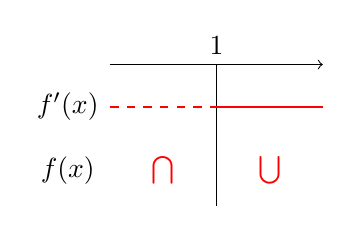
\begin{tikzpicture}[scale=0.9]
                    \draw[->](0,0)--(3,0);
                    \draw(1.5,0) node[above]{$1$}--(1.5,-2);
                    \node at (-0.6, -0.60){$f'(x)$};
                    \node at (-0.6, -1.50){$f(x)$};
                    \node[red] at (0.75,-1.50) {$\bigcap$};
                    \node[red] at (2.25,-1.50) {$\bigcup$};
                    \node[red] at (1.5, -0.60) {$\nexists$};
                    \draw[red,dashed] (0,-0.6)--(1.5,-0.6);
                    \draw[red] (1.5,-0.6)--(3,-0.6);
                \end{tikzpicture}
            \end{center}
        \item \textbf{Estremi globali: }per quanto detto precedentemente possiamo affermare che la funzione è illimitata sia inferiormente che superiormente. Non emmette perciò estremi globali.
        \item \textbf{Grafico:} ora abbiamo tutte le informazioni sufficienti per completare il grafico della funzione. Se abbiamo svolto il lavoro correttamente, ogni informazione acquisita deve essere stata confermata dalle precedenti. Si consiglia di aggiornare il disegno per ogni nuova informazione acquisita in modo da confrontarla con le precedenti. Anche per questo è stato scelto di proporre questo ordine.
        \begin{center}
            \begin{tikzpicture}[line cap=round,line join=round,>=triangle 45,x=1.0cm,y=1.0cm]
            \begin{axis}[
            x=1.0cm,y=1.0cm,
            axis lines=middle,
            ymajorgrids=true,
            xmajorgrids=true,
            xmin=-5.5,
            xmax=7.5,
            ymin=-3.5,
            ymax=6.5,
            xtick={-5.0,-4.0,...,7.0},
            ytick={-3.0,-2.0,...,6.0},]
            \clip(-5.5,-3.5) rectangle (7.5,6.5);
            \fill[line width=0.pt,color=blue,fill=blue,fill opacity=0.10000000149011612] (1.,0.) -- (1.,15.043627143200652) -- (-14.043627143200649,15.043627143200652) -- (-14.043627143200652,0.) -- cycle;
            \fill[line width=0.pt,color=blue,fill=blue,fill opacity=0.10000000149011612] (1.,0.) -- (1.,-15.043627143200652) -- (16.043627143200645,-15.043627143200654) -- (16.043627143200652,0.) -- cycle;
            \draw[line width=2.pt,color=teal,smooth,samples=100,domain=-5.5:0.9] plot(\x,{(\x)^(2)/((\x)-1)});
            \draw[line width=2.pt,color=teal,smooth,samples=100,domain=1.1:5.5] plot(\x,{(\x)^(2)/((\x)-1)});
            \draw[line width=1.pt,dash pattern=on 5pt off 5pt,color=red,smooth,samples=100,domain=-5.5:5.5] plot(\x,{(\x)+1});
            \draw [line width=1.pt,dash pattern=on 5pt off 5pt,color=red] (1.,-3.5) -- (1.,6.5);
            \draw [line width=0.pt,color=blue] (1.,0.)-- (1.,15.043627143200652);
            \draw [line width=0.pt,color=blue] (1.,15.043627143200652)-- (-14.043627143200649,15.043627143200652);
            \draw [line width=0.pt,color=blue] (-14.043627143200649,15.043627143200652)-- (-14.043627143200652,0.);
            \draw [line width=0.pt,color=blue] (-14.043627143200652,0.)-- (1.,0.);
            \begin{scriptsize}
            \draw [fill=black] (0.,0.) circle (2.5pt);
            \draw[color=black] (0.2,0.3) node {$O$};
            \draw [fill=black] (2.,4.) circle (2.5pt);
            \draw[color=black] (2.2,4.3) node {$M$};
            \end{scriptsize}
            \end{axis}
            \end{tikzpicture}
        \end{center}
        \end{enumerate}
    \end{ex}

    \begin{ex}
        [Studiare la funzione $y=x-\sqrt{x^2+4x}$, tralasciando la derivata seconda.]
        \begin{enumerate}
            \item \textbf{Classificazione:} funzione algebrica razionale fratta.
            \item \textbf{Dominio:} $x^3+4x\geq 0\ \ \Harr \ \ x(x+4)\geq 0\ \ ]-\infty;-4]\ \cup \ [0;+\infty[$
            \item \textbf{Simmetrie:} la condizione necessaria non è rispettata, per cui la funzione non è né pari né dispari.
            \item \textbf{Intersezioni con gli assi:} 
            \[\begin{cases}
                y=0\\
                y=f(x)
            \end{cases}\ \Harr \ \ x-\sqrt{x^2+4x}=0\ \ \Harr \ \ \sqrt{x^2+4x}=x\ \ \Harr\ \ \begin{cases}
                x(x+4)\geq 0\\
                x\geq 0\\
                x^2+4x=x^2
            \end{cases}\ \ \Harr\ \ \begin{cases}
                x\geq 0\\
                4x=0
            \end{cases}\]
            Per cui la funzione interseca gli assi cartesiani nell'origine $O(0,0)$.
            \item \textbf{Segno: }$f(x)>0$
            \[x-\sqrt{x^2+4x}>0\ \ \Harr\ \  \sqrt{x^2+4x}<x \ \ \Harr \ \ \begin{cases}
                x^4+4x\geq 0\\
                x>0\\
                x^2+4x<x^2
            \end{cases}\ \ \Harr \ \ \begin{cases}
                x\leq -4 \lor \geq 0\\
                x>0\\
                x<0
            \end{cases}\Harr\ \varnothing\]
            Per cui la funzione è negativa in tutto il suo dominio.
            \item \textbf{Limiti, asintoti e discontinuità:} Dobbiamo calcolare i limiti agli estremi del dominio.
            \[\lim_{x\to-\infty}\left( x-\sqrt{x^2+4x} \right)=-\infty\]
            È verificata la condizione necessaria per la presenza dell'asintoto obliquo. Procediamo con la verifica:
            \[m=\lim_{x\to -\infty}\frac{x-\sqrt{x^2-4x}}{x}=\left[ \frac{\infty}{\infty} \right]\underset{ger.}{\overset{FI}{=}}\lim_{x\to -\infty}\frac{x-\sqrt{x^2}}{x}=\lim_{x\to -\infty}\frac{x-|x|}{x}=\lim_{x\to -\infty}\frac{2x}{x}=2\]
            \[\begin{aligned}
                q&=\lim_{x\to -\infty}\left(x-\sqrt{x^2-4x}-2x\right)=\lim_{x\to -\infty}\left(-\sqrt{x^2-4x}-x\right)=\left[{-\infty+\infty} \right]\overset{FI}{=}\\
                &=\lim_{x\to-\infty}-\frac{x^2+4x-x^2}{\sqrt{x^2+4x}-x}\underset{ger.}{=}\lim_{x\to-\infty}-\frac{4x}{\sqrt{x^2}-x}= \lim_{x\to-\infty}-\frac{4x}{|x|-x}= \lim_{x\to-\infty}-\frac{4x}{-x-x}= 2
            \end{aligned}\]
            La funzione presenta quindi un asintoto obliquo sinistro alla retta $y=2x+2$.
            \[\lim_{x\to -4^-}\left( x-\sqrt{x^2+4x} \right)=-4^-\qquad \qquad f(-4)=-4\]
            la funzione è quindi continua da sinistra in $x=-4$;
            \[\lim_{x\to 0^+}\left( x-\sqrt{x^2+4x} \right)=0^-\qquad \qquad f(0)=0\]
            la funzione è quindi continua da destra in $x=0$.
            \[\begin{aligned}\lim_{x\to+\infty}\left( x-\sqrt{x^2+4x} \right)&=\left[{-\infty+\infty} \right]\overset{FI}{=}\lim_{x\to+\infty}\frac{x^2-x^2-4x}{x+\sqrt{x^2+4x}}=\left[ \frac{\infty}{\infty} \right]\underset{ger.}{\overset{FI}{=}}\lim_{x\to+\infty}\frac{-4x}{x+\sqrt{x^2}}=\\&=\lim_{x\to +\infty}\frac{-4x}{2x}=-2\end{aligned}\]
            La funzione presenta quindi un asintoto orizzontale destro alla retta $y=2$.
            \item \textbf{Derivata prima: }
            \[y'=1-\frac{1}{2\sqrt{x^2+4x}}\left( 2x+4 \right)=\frac{\sqrt{x^2+4x}-x-2}{\sqrt{x^2+4x}}\]
            Determiniamo il dominio della derivata prima $\dom f'=]-\infty;-4[\ \cup \ ]0;+\infty[$ e osserviamo che differisce dal dominio della funzione per i punti $x=0$ e $x=-4$. Essi saranno dei punti di non derivabilità da classificare. Posso applicare il criterio di derivabilità:
            \[f'_-(-4)=\lim_{x\to -4^-}\frac{\sqrt{x^2+4x}-x-2}{\sqrt{x^2+4x}}=\left[\frac{2}{0^+}\right]=+\infty\qquad \qquad f'_+(-4)\ \nexists \text{ per dominio}\]
            la funzione presenta un punto a tangente verticale in $x=-4$;
            \[f'_-(0)\ \nexists \text{ per dominio}\qquad \qquad f'_+(0)=\lim_{x\to 0}\frac{\sqrt{x^2+4x}-x-2}{\sqrt{x^2+4x}}=\left[\frac{-2}{0^+}\right]=-\infty\]
            la funzione presenta un punto a tangente verticale in $x=0$. Cerchiamo ora eventuali punti stazionari:
            \[\frac{\sqrt{x^2+4x}-x-2}{\sqrt{x^2+4x}}=0\qquad {\sqrt{x^2+4x}=x+2}\qquad \begin{cases}
                x(x+4)\geq 0\\
                x\geq -2\\
                x^2-4x=x^2-4x+4
            \end{cases}\ \  \begin{cases}
                x(x+4)\geq 0\\
                x\geq -2\\
                0=4
            \end{cases}\]
            La funzione non ha quindi punti stazionari. Studiamo ora il segno della derivata:
            \begin{center}
                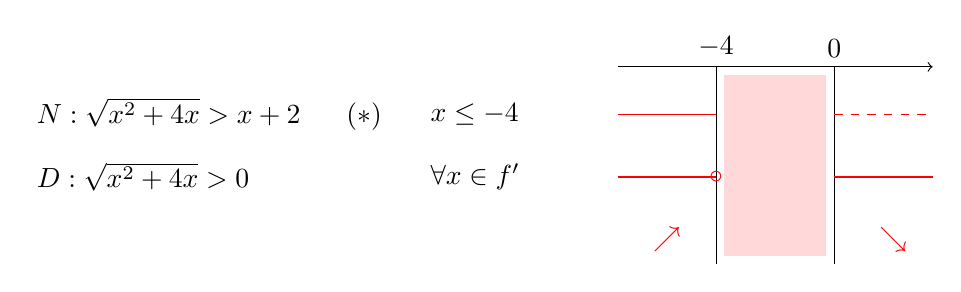
\begin{tikzpicture}
                    \fill [red!15] (8.85,0.9)--(8.85,-1.4)--(10.15,-1.4)--(10.15,0.9)--cycle;
                    \node at (0,0.4) [anchor=west]{$N: \sqrt{x^2+4x}>x+2\quad~~ (*)$};
                    \node at (0,-0.4)[anchor=west]{$D: \sqrt{x^2+4x}>0$};
                    \node at (5,0.4)[anchor=west]{$x\leq -4$};
                    \node at (5,-0.4)[anchor=west]{$\forall x \in \dom f'$};
                    \draw[->] (7.5,1)--(11.5,1);
                    \draw (8.75,1)node [above]{$-4$}--(8.75,-1.5);
                    \draw (10.25,1) node [above]{$0$}--(10.25,-1.5);
                    %%riga 1
                    \draw [color=red] (7.5, 0.4)--(8.75,0.4);
                    \node [color=red] at (8.75,0.4){$\nexists$};
                    \draw [color=red, dashed] (10.25, 0.4)--(11.5,0.4);
                    \node [color=red] at (10.25,0.4){$\nexists$};
                    %% riga 2
                    \draw[color=red] (7.5, -0.4)--(8.75,-0.4) node {$\circ$};
                    \draw [color=red] (10.25, -0.4)--(11.5,-0.4);
                    
                    \node [color=red]at (8.125,-1.2){$\nearrow$};
                    \node [color=red]at (11,-1.2){$\searrow$};
                \end{tikzpicture}
            \end{center}
            \[(*)\qquad \begin{cases}
                x^2+4x\geq 0\\x+2\geq 0\\ x^2+4x>(x+2)^2
            \end{cases}\quad \cup \qquad \begin{cases}
                x^2+4x\geq 0\\x+2<0\\\forall x \in \R
            \end{cases}\]
            \[\varnothing\quad \cup \quad x\leq -4\]
            \addtocounter{enumi}{1} % skip derivata seconda
            \item \textbf{Estremi globali: } La funzione ha punti di massimo globali in $x=-4$ e $x=0$; è illimitata inferiormente.
            \item \textbf{Disegno: }
            \begin{center}
                \begin{tikzpicture}[line cap=round,line join=round,>=triangle 45,x=1.0cm,y=1.0cm]
                \begin{axis}[
                x=1.0cm,y=1.0cm,
                axis lines=middle,
                ymajorgrids=true,
                xmajorgrids=true,
                xmin=-6.5,
                xmax=5.5,
                ymin=-7.5,
                ymax=1.5,
                xtick={-6.0,-5.0,...,5.0},
                ytick={-7.0,-6.0,...,1.0},]
                \clip(-7.5,-7.5) rectangle (7.5,1.5);
                \fill[line width=0.pt,color=blue,fill=blue,fill opacity=0.10000000149011612](0,0)--(6,0)--(6,2)--(0,2)--cycle;
                \fill[line width=0.pt,color=blue,fill=blue,fill opacity=0.10000000149011612](-4,0)--(-6.5,0)--(-6.5,2)--(-4,2)--cycle;
                \fill[line width=1.5pt,dash pattern=on 5pt off 2pt,color=red,fill=red,fill opacity=0.10000000149011612] (-4.,8.) -- (0.,8.) -- (0.,-18.) -- (-4.,-18.) -- cycle;
                \draw[line width=2.pt,color=teal,smooth,samples=100,domain=-5.5:-4.000000069999991] plot(\x,{(\x)-sqrt((\x)^(2.0)+4*(\x))});
                \draw[line width=2.pt,color=teal,smooth,samples=100,domain=9.248943717311174E-6:5.5] plot(\x,{(\x)-sqrt((\x)^(2.0)+4*(\x))});
                \draw[line width=1.5pt,dash pattern=on 5pt off 5pt,color=red,smooth,samples=100,domain=-5.5:-4] plot(\x,{2*(\x)+2});
                \draw [line width=1.5pt,dash pattern=on 5pt off 5pt,color=red,domain=0:5.5] plot(\x,{(-2.-0.*\x)/1.});
                \draw [line width=1.5pt,dash pattern=on 5pt off 5pt,color=red] (-4.,8.)-- (0.,8.);
                \draw [line width=1.5pt,dash pattern=on 5pt off 5pt,color=red] (0.,8.)-- (0.,-18.);
                \draw [line width=1.5pt,dash pattern=on 5pt off 5pt,color=red] (0.,-18.)-- (-4.,-18.);
                \draw [line width=1.5pt,dash pattern=on 5pt off 5pt,color=red] (-4.,-18.)-- (-4.,8.);
                \begin{scriptsize}
                \draw [fill=blue] (0.,0.) circle (2.5pt);
                \draw[color=blue] (0.11658212836203329,0.29260536954385497) node {$O$};
                \end{scriptsize}
                \end{axis}
                \end{tikzpicture}
            \end{center}
        \end{enumerate}
    \end{ex}

\section{Esercizi}
    \begin{exc}\label{exc: sfx 1}
        Studiare la funzione $\displaystyle g(x)=e^{\left|\frac{x+1}{x-1}\right|}$.\qquad {\hyperref[sol: sfx 1]{\footnotesize Soluzione a pag. \pageref*{sol: sfx 1}}}
    \end{exc}

    \begin{exc}\label{exc: sfx 2}
        Sia $g(x)=|x-1|e^{-\alpha x} ~~(\alpha>0)$. Fornire un grafico qualitativo di $g$.\qquad {\hyperref[sol: sfx 2]{\footnotesize Soluzione a pag. \pageref*{sol: sfx 2}}}
    \end{exc}

\include{soluzioni.tex}


\end{document}